\documentclass{article}\usepackage[]{graphicx}\usepackage[]{color}
%% maxwidth is the original width if it is less than linewidth
%% otherwise use linewidth (to make sure the graphics do not exceed the margin)
\makeatletter
\def\maxwidth{ %
  \ifdim\Gin@nat@width>\linewidth
    \linewidth
  \else
    \Gin@nat@width
  \fi
}
\makeatother

\definecolor{fgcolor}{rgb}{0.345, 0.345, 0.345}
\newcommand{\hlnum}[1]{\textcolor[rgb]{0.686,0.059,0.569}{#1}}%
\newcommand{\hlstr}[1]{\textcolor[rgb]{0.192,0.494,0.8}{#1}}%
\newcommand{\hlcom}[1]{\textcolor[rgb]{0.678,0.584,0.686}{\textit{#1}}}%
\newcommand{\hlopt}[1]{\textcolor[rgb]{0,0,0}{#1}}%
\newcommand{\hlstd}[1]{\textcolor[rgb]{0.345,0.345,0.345}{#1}}%
\newcommand{\hlkwa}[1]{\textcolor[rgb]{0.161,0.373,0.58}{\textbf{#1}}}%
\newcommand{\hlkwb}[1]{\textcolor[rgb]{0.69,0.353,0.396}{#1}}%
\newcommand{\hlkwc}[1]{\textcolor[rgb]{0.333,0.667,0.333}{#1}}%
\newcommand{\hlkwd}[1]{\textcolor[rgb]{0.737,0.353,0.396}{\textbf{#1}}}%

\usepackage{framed}
\makeatletter
\newenvironment{kframe}{%
 \def\at@end@of@kframe{}%
 \ifinner\ifhmode%
  \def\at@end@of@kframe{\end{minipage}}%
  \begin{minipage}{\columnwidth}%
 \fi\fi%
 \def\FrameCommand##1{\hskip\@totalleftmargin \hskip-\fboxsep
 \colorbox{shadecolor}{##1}\hskip-\fboxsep
     % There is no \\@totalrightmargin, so:
     \hskip-\linewidth \hskip-\@totalleftmargin \hskip\columnwidth}%
 \MakeFramed {\advance\hsize-\width
   \@totalleftmargin\z@ \linewidth\hsize
   \@setminipage}}%
 {\par\unskip\endMakeFramed%
 \at@end@of@kframe}
\makeatother

\definecolor{shadecolor}{rgb}{.97, .97, .97}
\definecolor{messagecolor}{rgb}{0, 0, 0}
\definecolor{warningcolor}{rgb}{1, 0, 1}
\definecolor{errorcolor}{rgb}{1, 0, 0}
\newenvironment{knitrout}{}{} % an empty environment to be redefined in TeX

\usepackage{alltt}
\usepackage{graphicx}
\usepackage[left=1.00in, right=1.00in, top=1.00in, bottom=1.00in]{geometry}
\usepackage{hyperref}

\hypersetup{
    colorlinks,
    citecolor=black,
    filecolor=black,
    linkcolor=blue,
    urlcolor=black
}

\DeclareGraphicsExtensions{.png,.jpg}

\title{Experiment Outputs}
\author{Daniel Chen \\ Mailman School of Public health \\ Columbia University}
\date{}



\IfFileExists{upquote.sty}{\usepackage{upquote}}{}

\begin{document}
\maketitle
\tableofcontents

\newpage
\section{Output}
% \subsection{Output 1}
% \label{sec:output1}
% Output Data
% \begin{itemize}
%   \item Agents Activated: 1
%   \item Valence Bank: both
%   \begin{itemize}
%       \item Valence bank activation: random
%   \end{itemize}
%   \item Valence bank Weights: random
%   \begin{itemize}
%       \item opposite -0.2
%       \item corresponding 0.5
%       \item carry over = 0.2
%       \item bias = 0
%       \item decay = -0.5
%   \end{itemize}
%   \item Network: circle
%   \item Random number: read in from file
%   \item Processing units per valence bank: 5
%   \item number of agents: 10
%   \item number of time ticks: 10,000
% \end{itemize}
%
% \subsubsection{First 100 time ticks}
% <<plot-output-1, fig.cap="Output 1, first 100 time ticks", fig.show='asis'>>=
% plot.thesis.data("/home/dchen/git/repast-neural-network-agent-based-model/R/data/agent1-both-random-weights-10k.csv", 10, 10000, 1, 0, 100)
% @
%
% \newpage
% \subsubsection{All time ticks}
% <<plot-output-1a, fig.cap="Output 1, all time ticks", fig.show='asis'>>=
% plot.thesis.data("/home/dchen/git/repast-neural-network-agent-based-model/R/data/agent1-both-random-weights-10k.csv", 10, 10000)
% @
%
% \newpage
% \subsection{Exp1a}
% \subsubsection{First 5 time ticks}
% <<plot-exp1a, fig.cap="Exp1a, first 100 time ticks", fig.show='asis'>>=
% plot.thesis.data("/home/dchen/git/repast-neural-network-agent-based-model/R/data/exp1a.csv", 40, 1000, 1, 0, 5)
% @
%
% \newpage
% \subsubsection{All time ticks}
% <<plot-exp1a1, fig.cap="Exp1a, all time ticks", fig.show='asis'>>=
% plot.thesis.data("/home/dchen/git/repast-neural-network-agent-based-model/R/data/exp1a.csv", 40, 1000)
% @

\newpage
\subsection{Exp1b}
\subsubsection{First 5 time ticks}
\begin{knitrout}
\definecolor{shadecolor}{rgb}{0.969, 0.969, 0.969}\color{fgcolor}\begin{kframe}
\begin{alltt}
\hlkwd{source}\hlstd{(}\hlkwc{file} \hlstd{=} \hlstr{"../plot-function-ggplot2.R"}\hlstd{)}
\hlkwd{plot.multiple.run.data}\hlstd{(}\hlstr{"../data/exp/exp1b.csv"}\hlstd{,} \hlkwc{numAgents} \hlstd{=} \hlnum{100}\hlstd{,} \hlkwc{numTimeTicks} \hlstd{=} \hlnum{100}\hlstd{,}
    \hlkwc{limit.x} \hlstd{=} \hlkwd{c}\hlstd{(}\hlstr{"yes"}\hlstd{,} \hlnum{0}\hlstd{,} \hlnum{5}\hlstd{))}
\end{alltt}
\begin{verbatim}
## [1] 1
## [1] 1
\end{verbatim}


{\ttfamily\noindent\itshape\color{messagecolor}{\#\# Loading required package: ggplot2\\\#\# Loading required package: scales\\\#\# Scale for 'x' is already present. Adding another scale for 'x', which will replace the existing scale.}}

{\ttfamily\noindent\color{warningcolor}{\#\# Warning: Removed 9400 rows containing missing values (geom\_path).\\\#\# Warning: Removed 9400 rows containing missing values (geom\_path).}}\begin{verbatim}
## [1] 2
## [1] 10001
\end{verbatim}


{\ttfamily\noindent\itshape\color{messagecolor}{\#\# Scale for 'x' is already present. Adding another scale for 'x', which will replace the existing scale.}}\end{kframe}
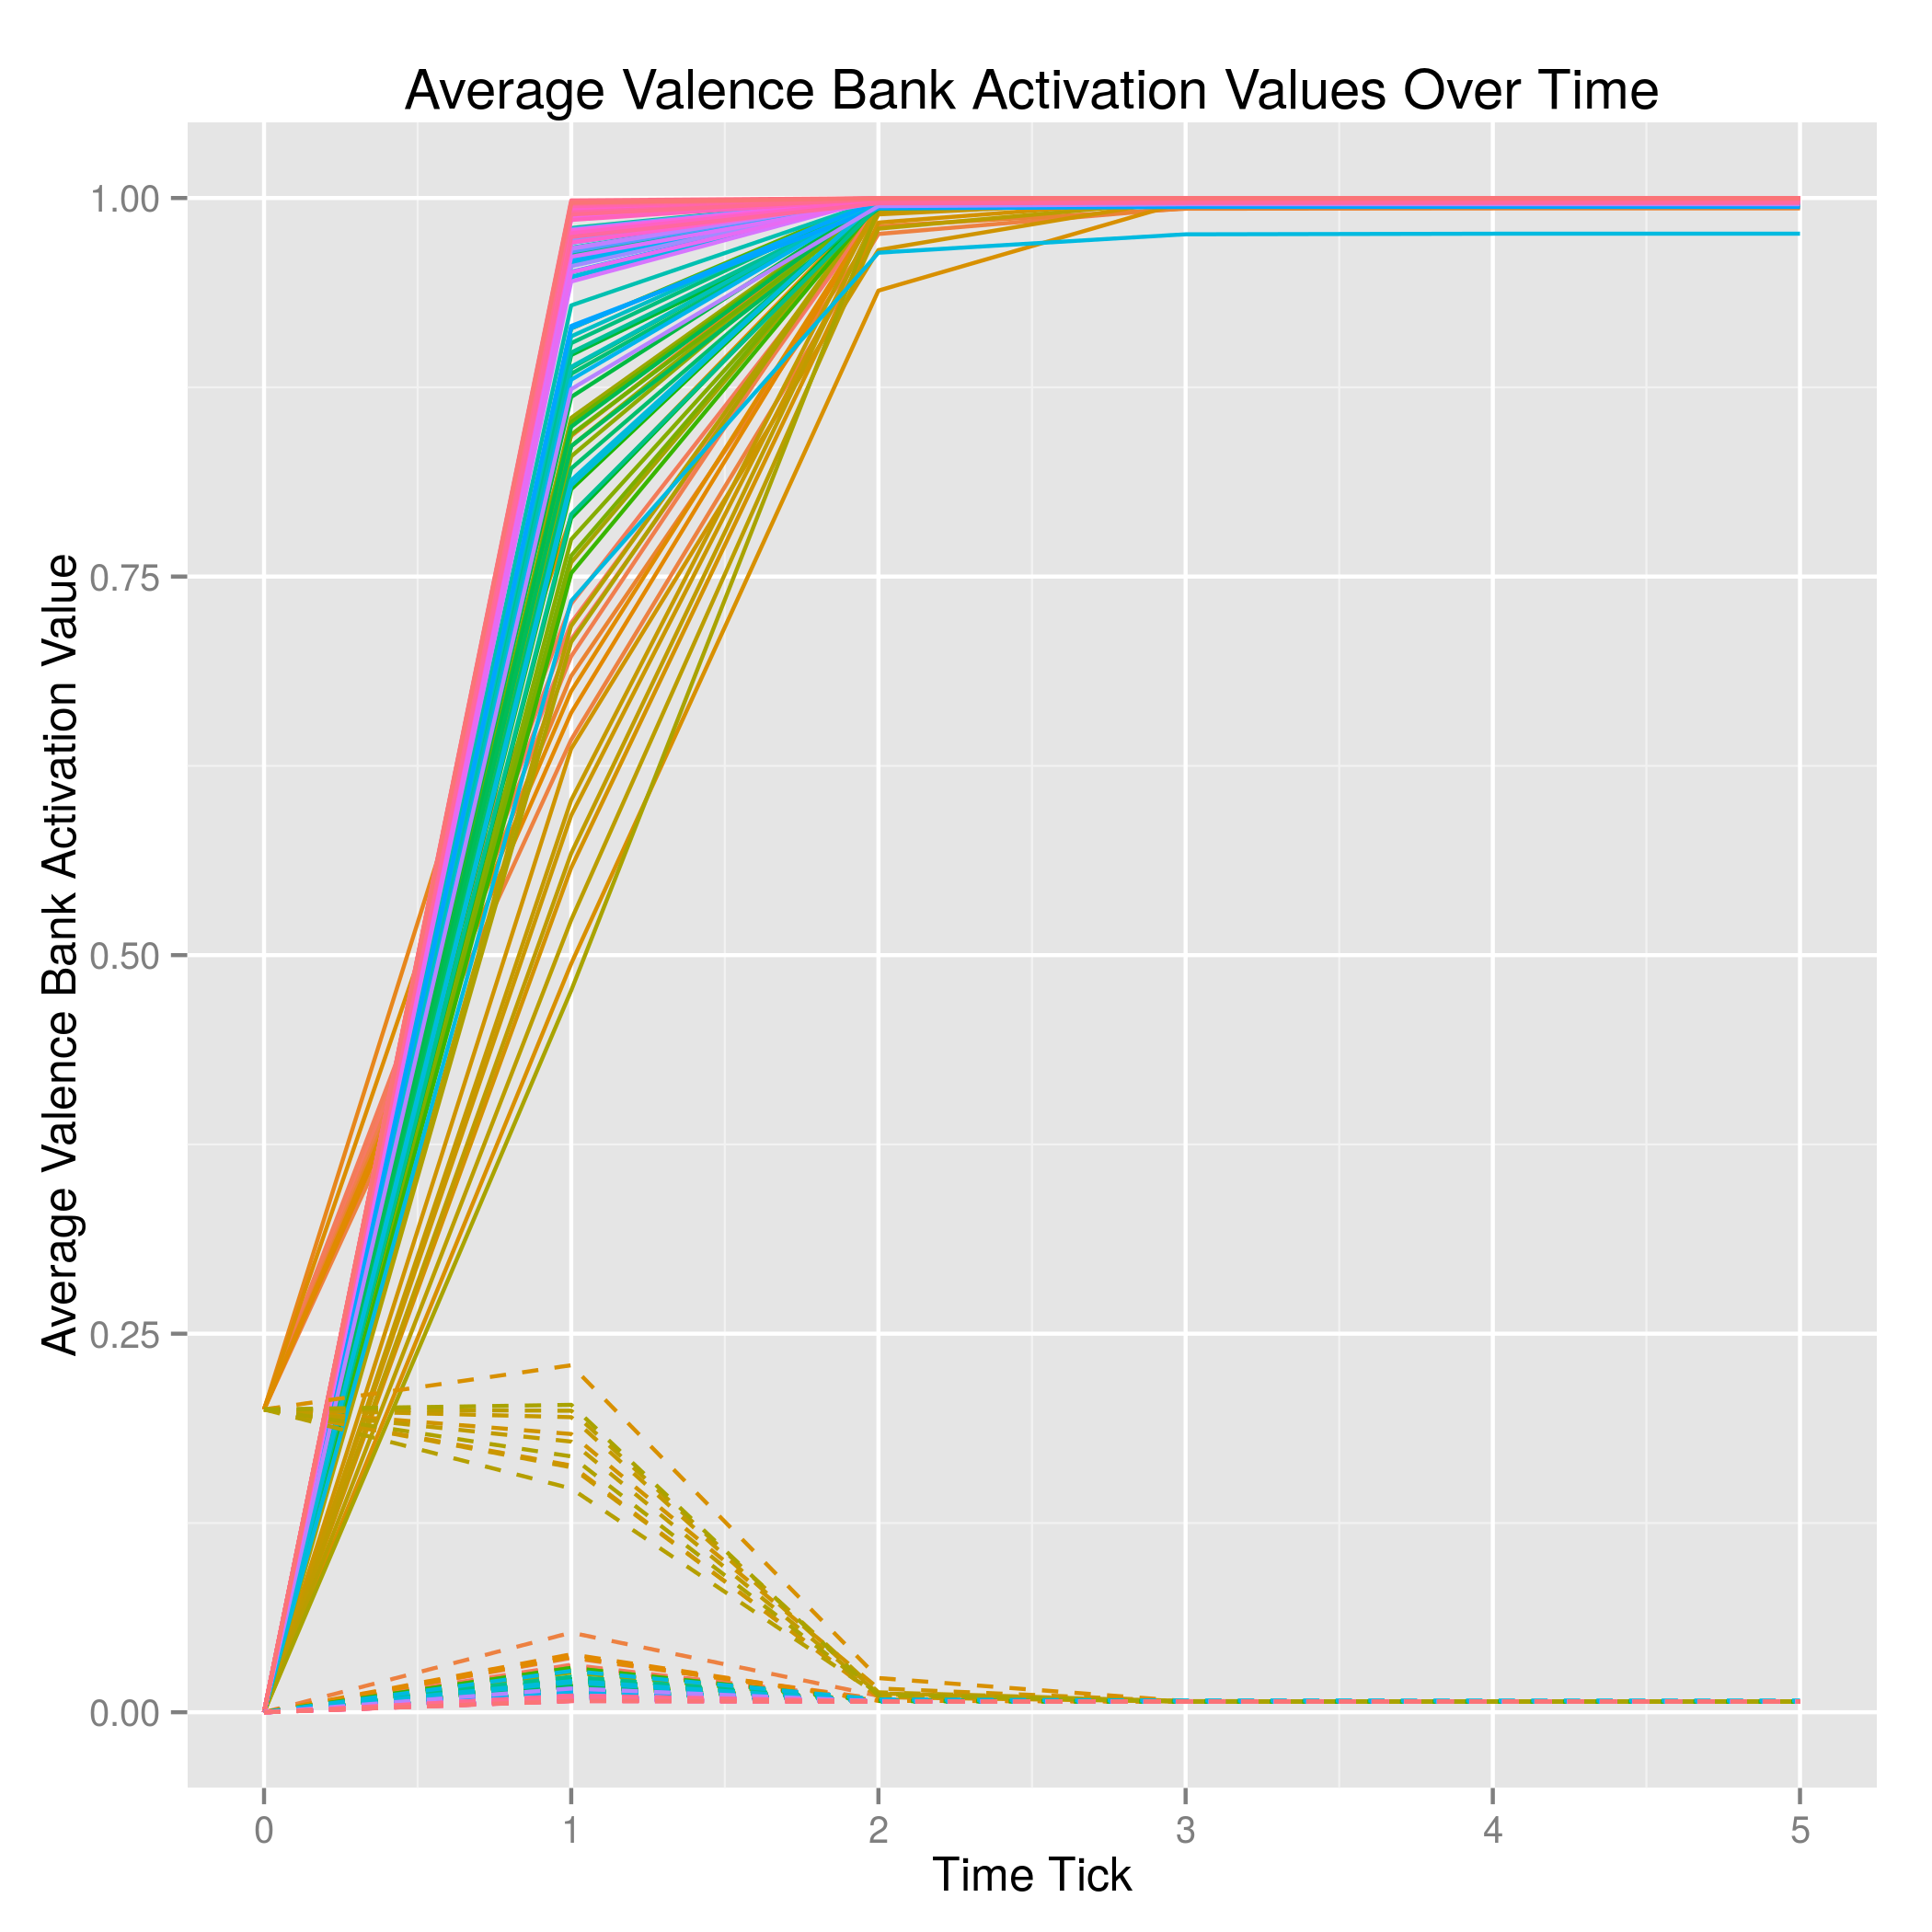
\includegraphics[width=\maxwidth]{figure/unnamed-chunk-11} 
\begin{kframe}

{\ttfamily\noindent\color{warningcolor}{\#\# Warning: Removed 9400 rows containing missing values (geom\_path).\\\#\# Warning: Removed 9400 rows containing missing values (geom\_path).}}\begin{verbatim}
## [1] 3
## [1] 20001
\end{verbatim}


{\ttfamily\noindent\itshape\color{messagecolor}{\#\# Scale for 'x' is already present. Adding another scale for 'x', which will replace the existing scale.}}\end{kframe}
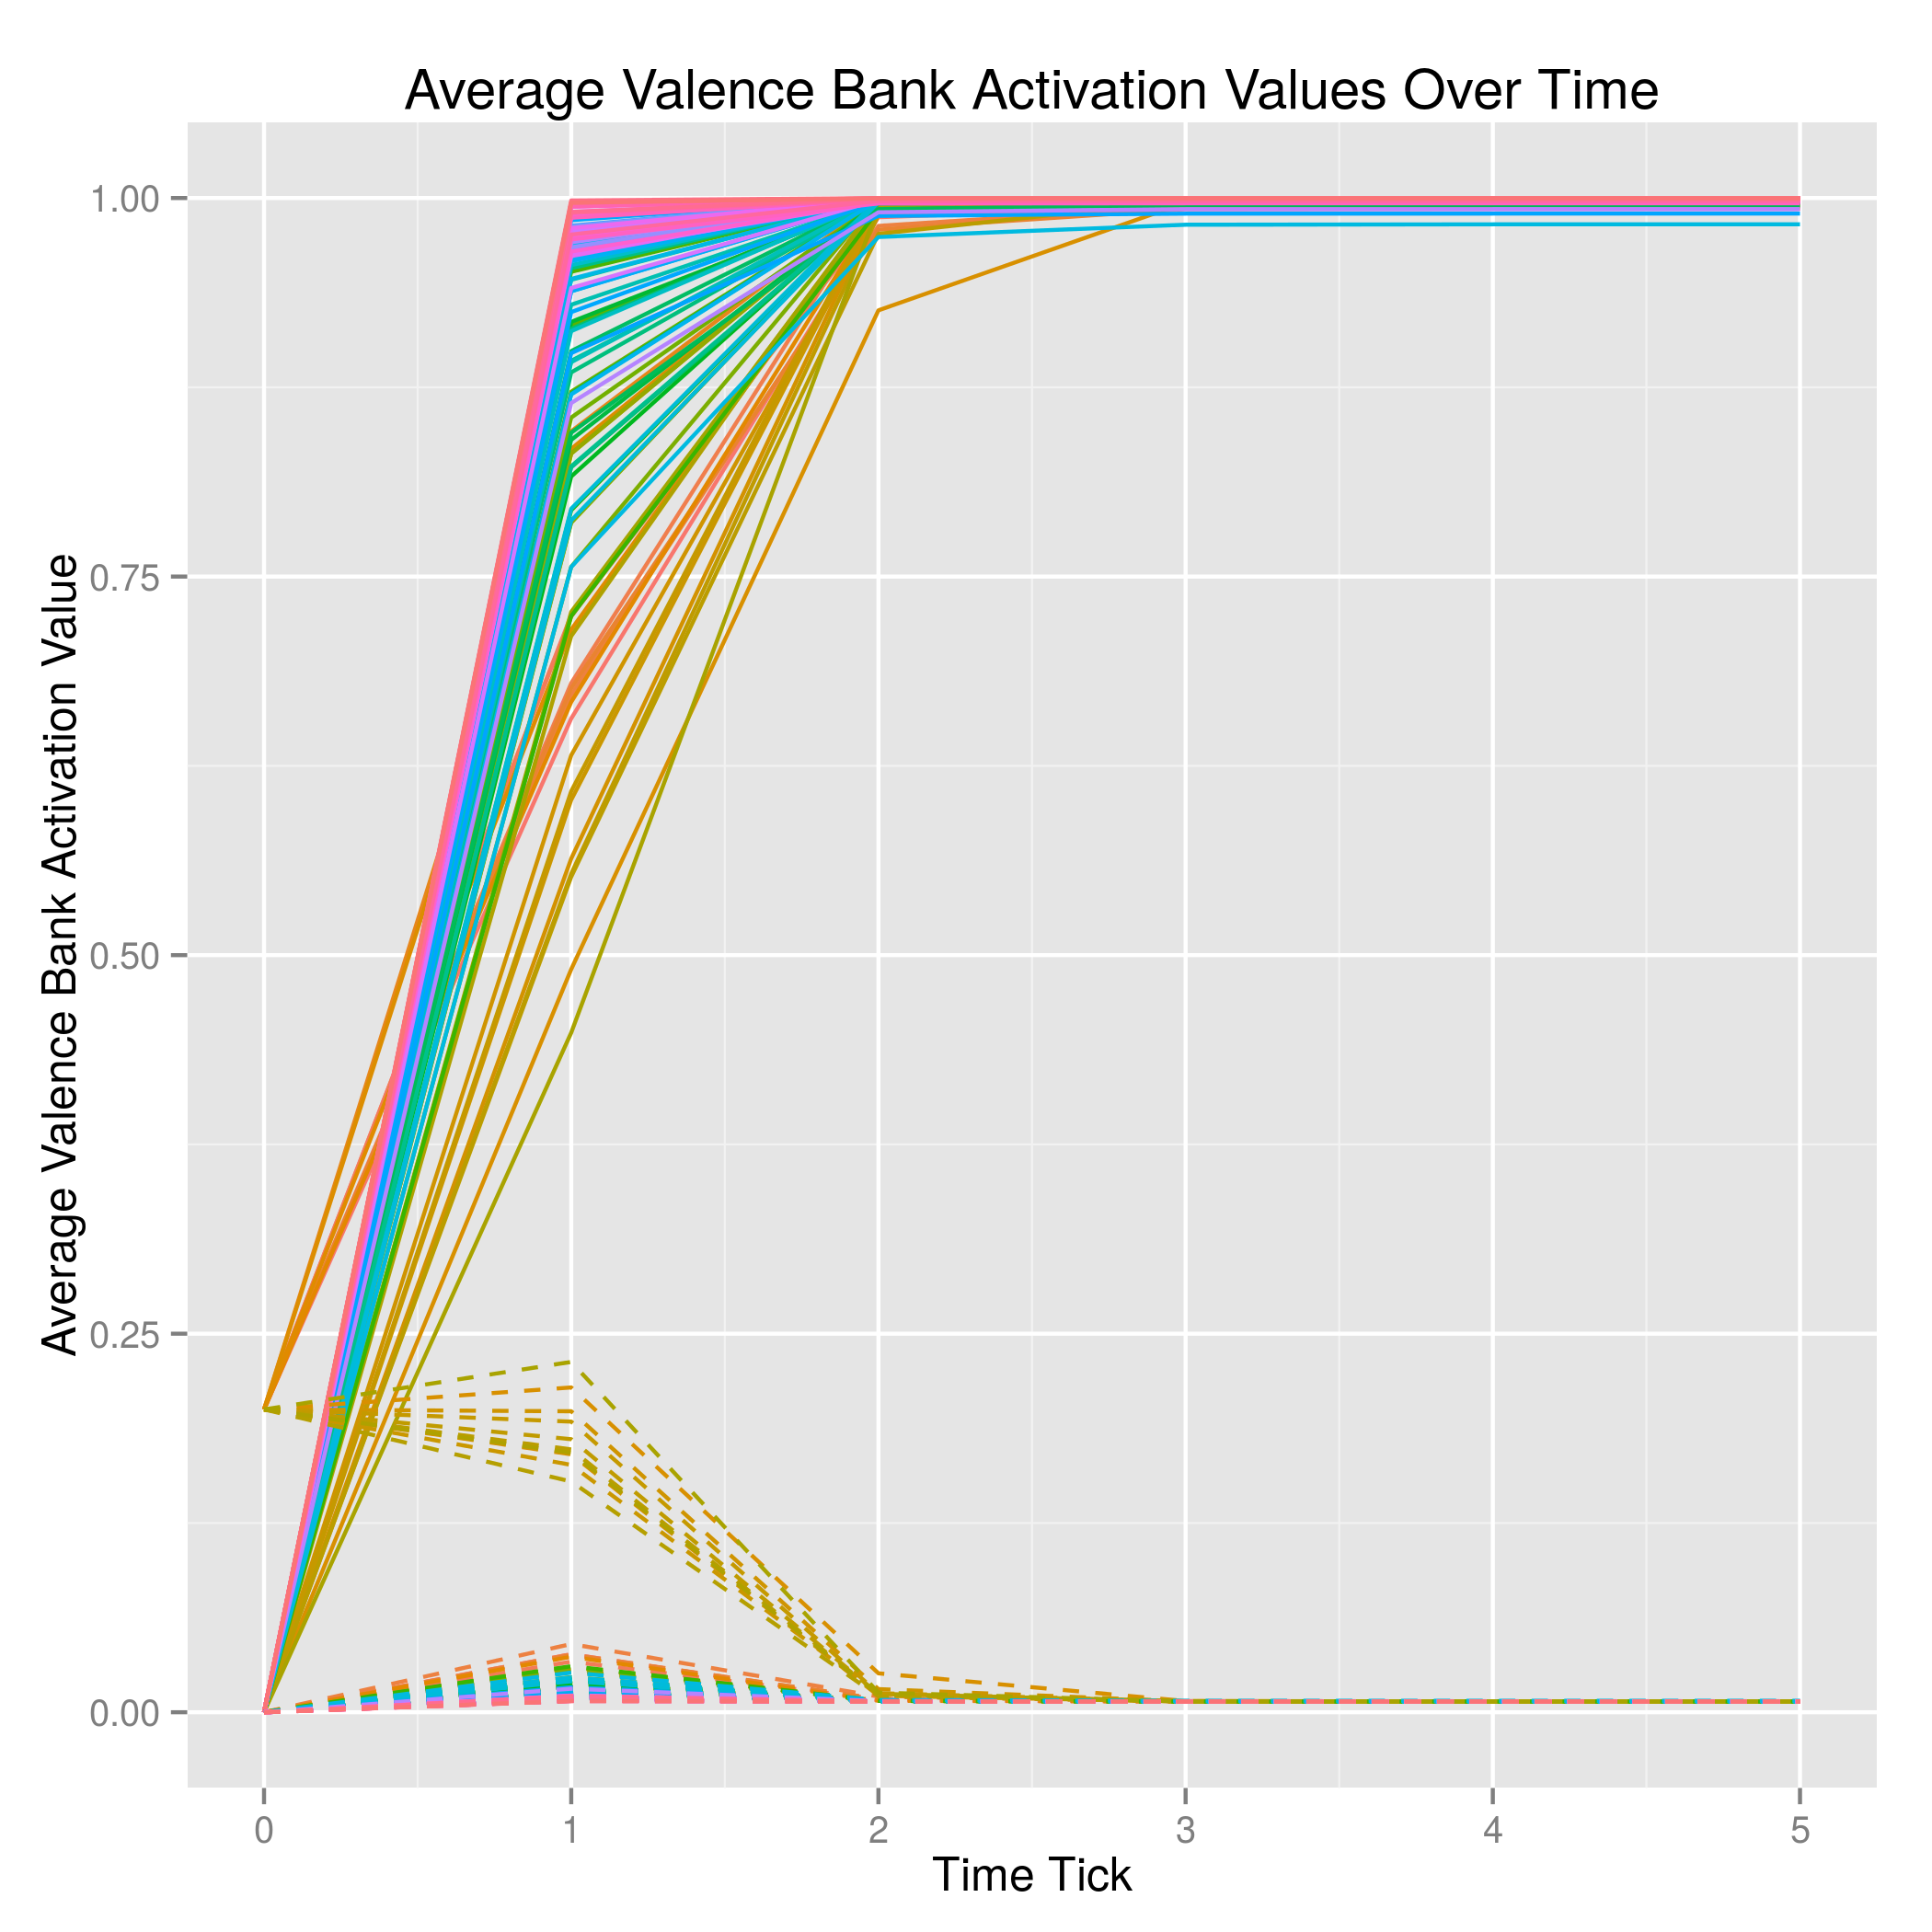
\includegraphics[width=\maxwidth]{figure/unnamed-chunk-12} 
\begin{kframe}

{\ttfamily\noindent\color{warningcolor}{\#\# Warning: Removed 9400 rows containing missing values (geom\_path).\\\#\# Warning: Removed 9400 rows containing missing values (geom\_path).}}\begin{verbatim}
## [1] 4
## [1] 30001
\end{verbatim}


{\ttfamily\noindent\itshape\color{messagecolor}{\#\# Scale for 'x' is already present. Adding another scale for 'x', which will replace the existing scale.}}\end{kframe}
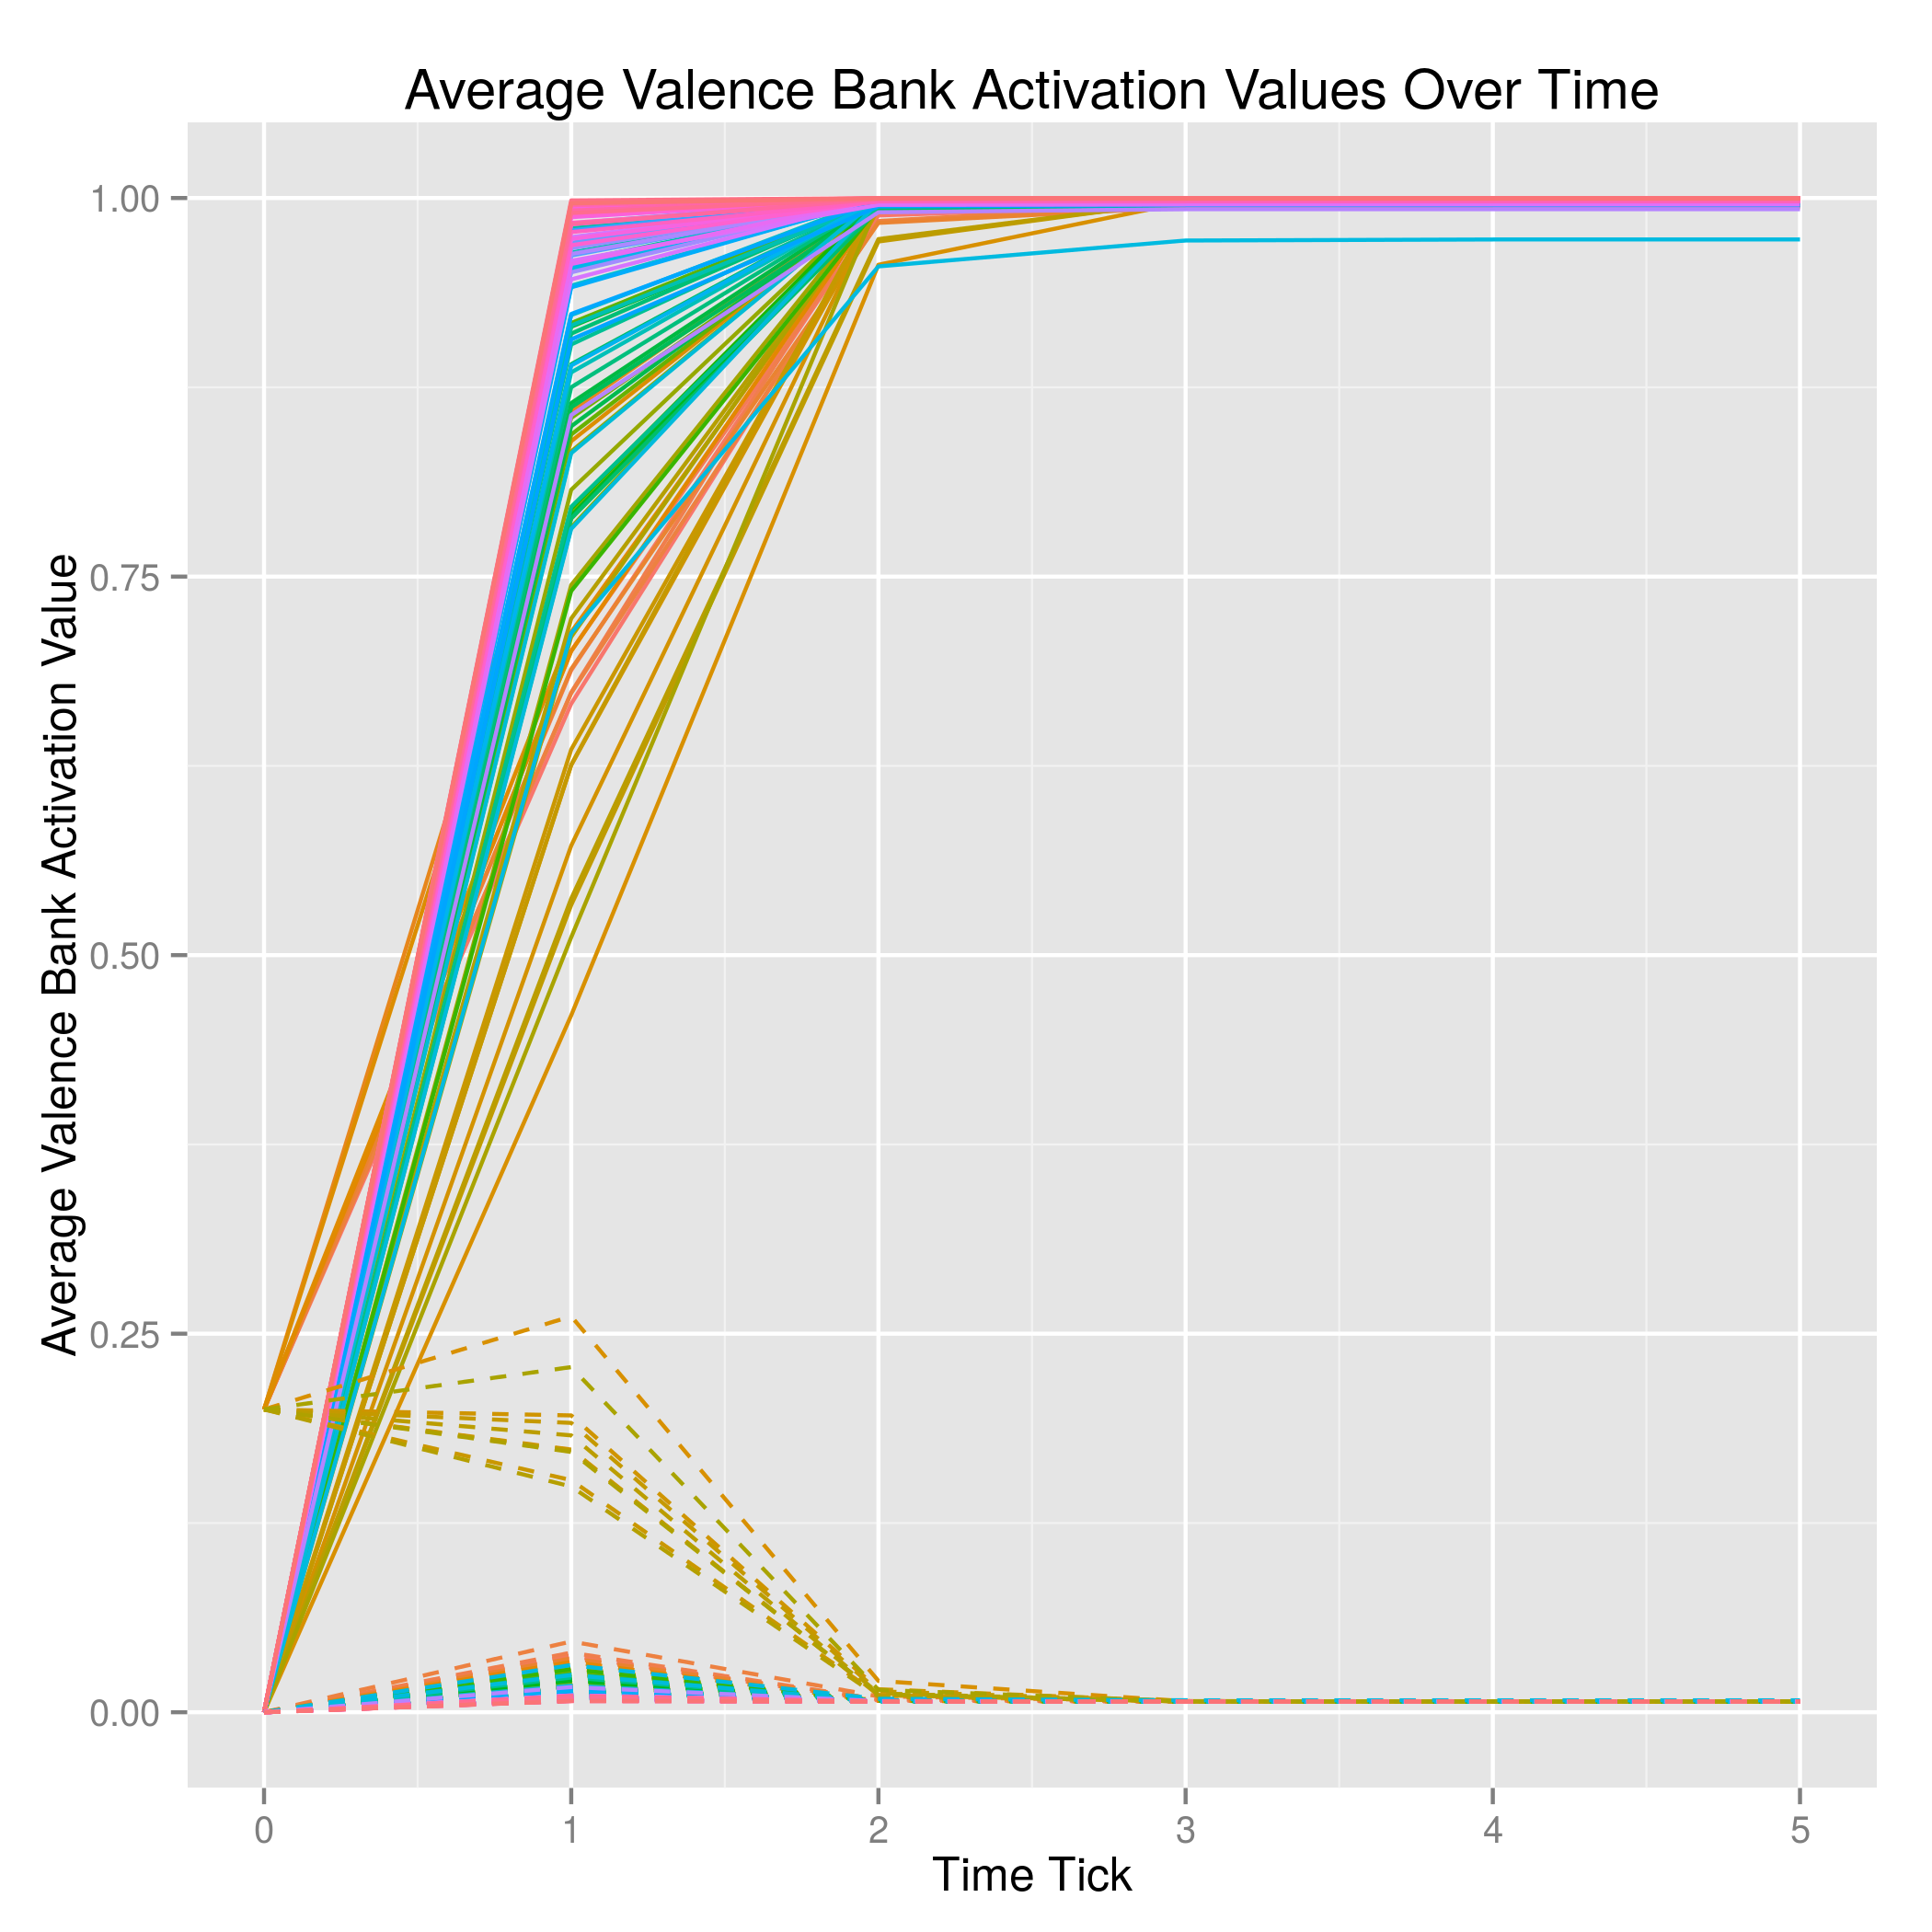
\includegraphics[width=\maxwidth]{figure/unnamed-chunk-13} 
\begin{kframe}

{\ttfamily\noindent\color{warningcolor}{\#\# Warning: Removed 9400 rows containing missing values (geom\_path).\\\#\# Warning: Removed 9400 rows containing missing values (geom\_path).}}\begin{verbatim}
## [1] 5
## [1] 40001
\end{verbatim}


{\ttfamily\noindent\itshape\color{messagecolor}{\#\# Scale for 'x' is already present. Adding another scale for 'x', which will replace the existing scale.}}\end{kframe}
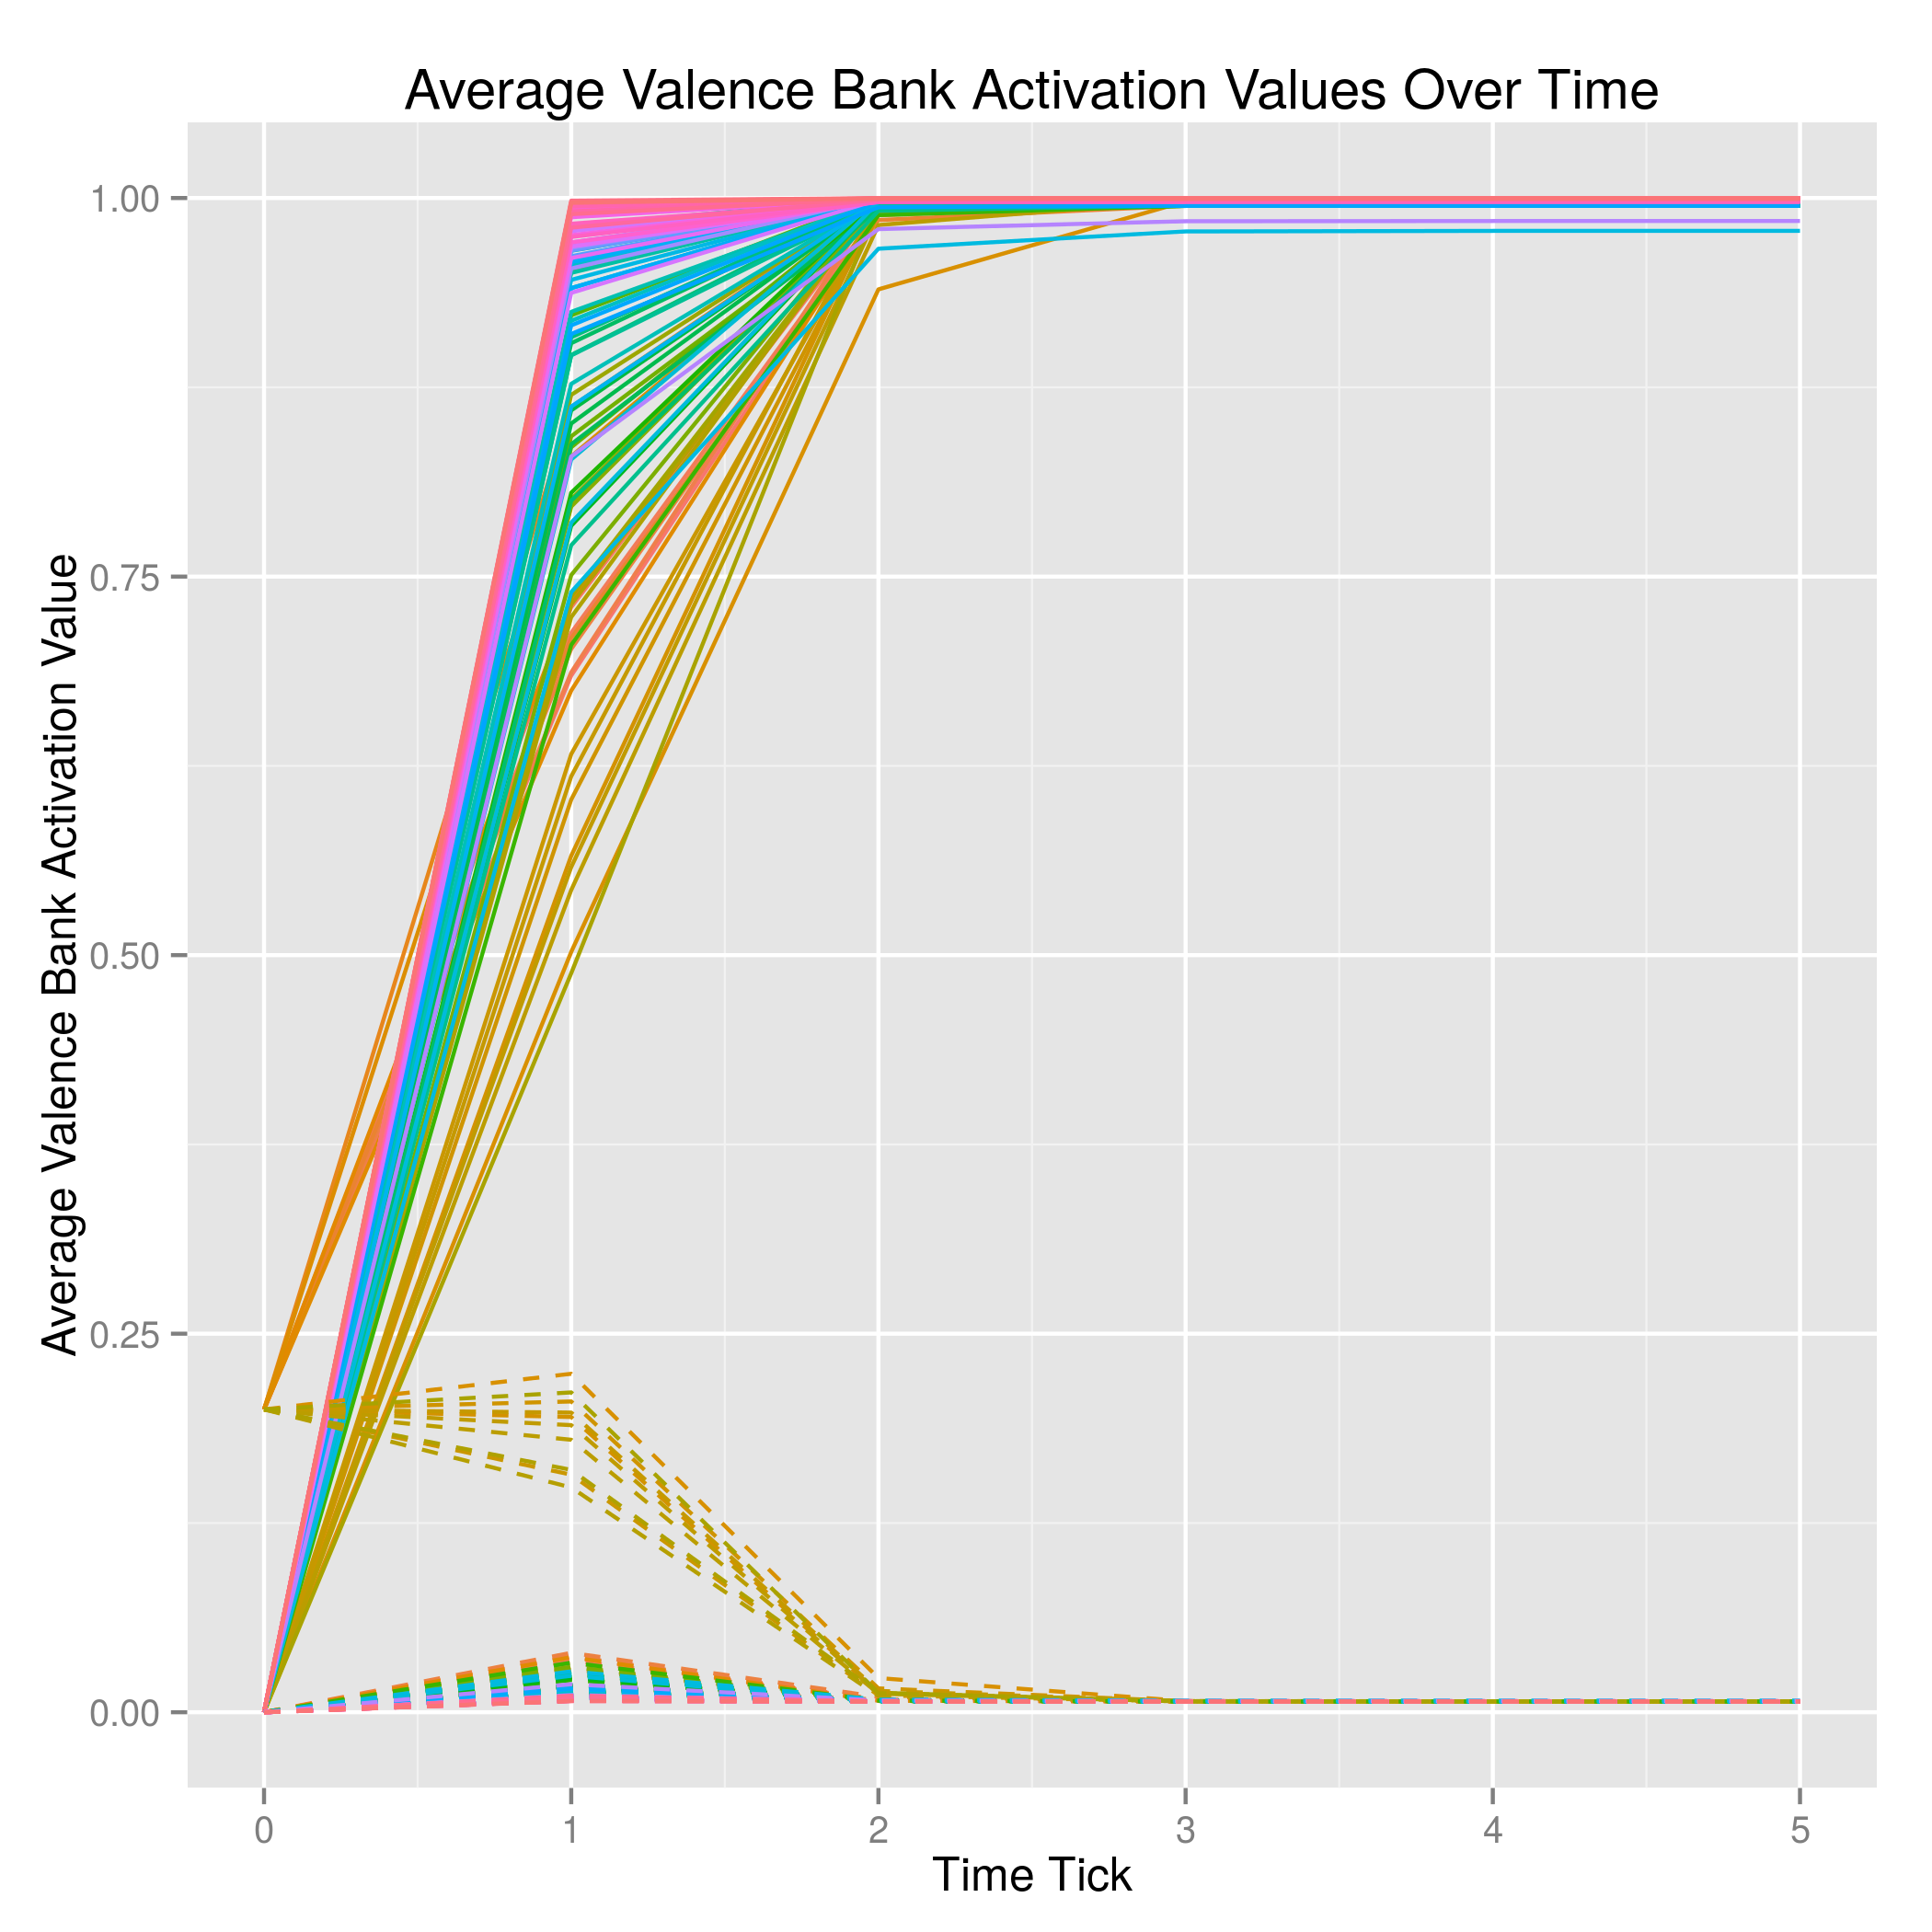
\includegraphics[width=\maxwidth]{figure/unnamed-chunk-14} 
\begin{kframe}

{\ttfamily\noindent\color{warningcolor}{\#\# Warning: Removed 9400 rows containing missing values (geom\_path).\\\#\# Warning: Removed 9400 rows containing missing values (geom\_path).}}\begin{verbatim}
## [1] 6
## [1] 50001
\end{verbatim}


{\ttfamily\noindent\itshape\color{messagecolor}{\#\# Scale for 'x' is already present. Adding another scale for 'x', which will replace the existing scale.}}\end{kframe}
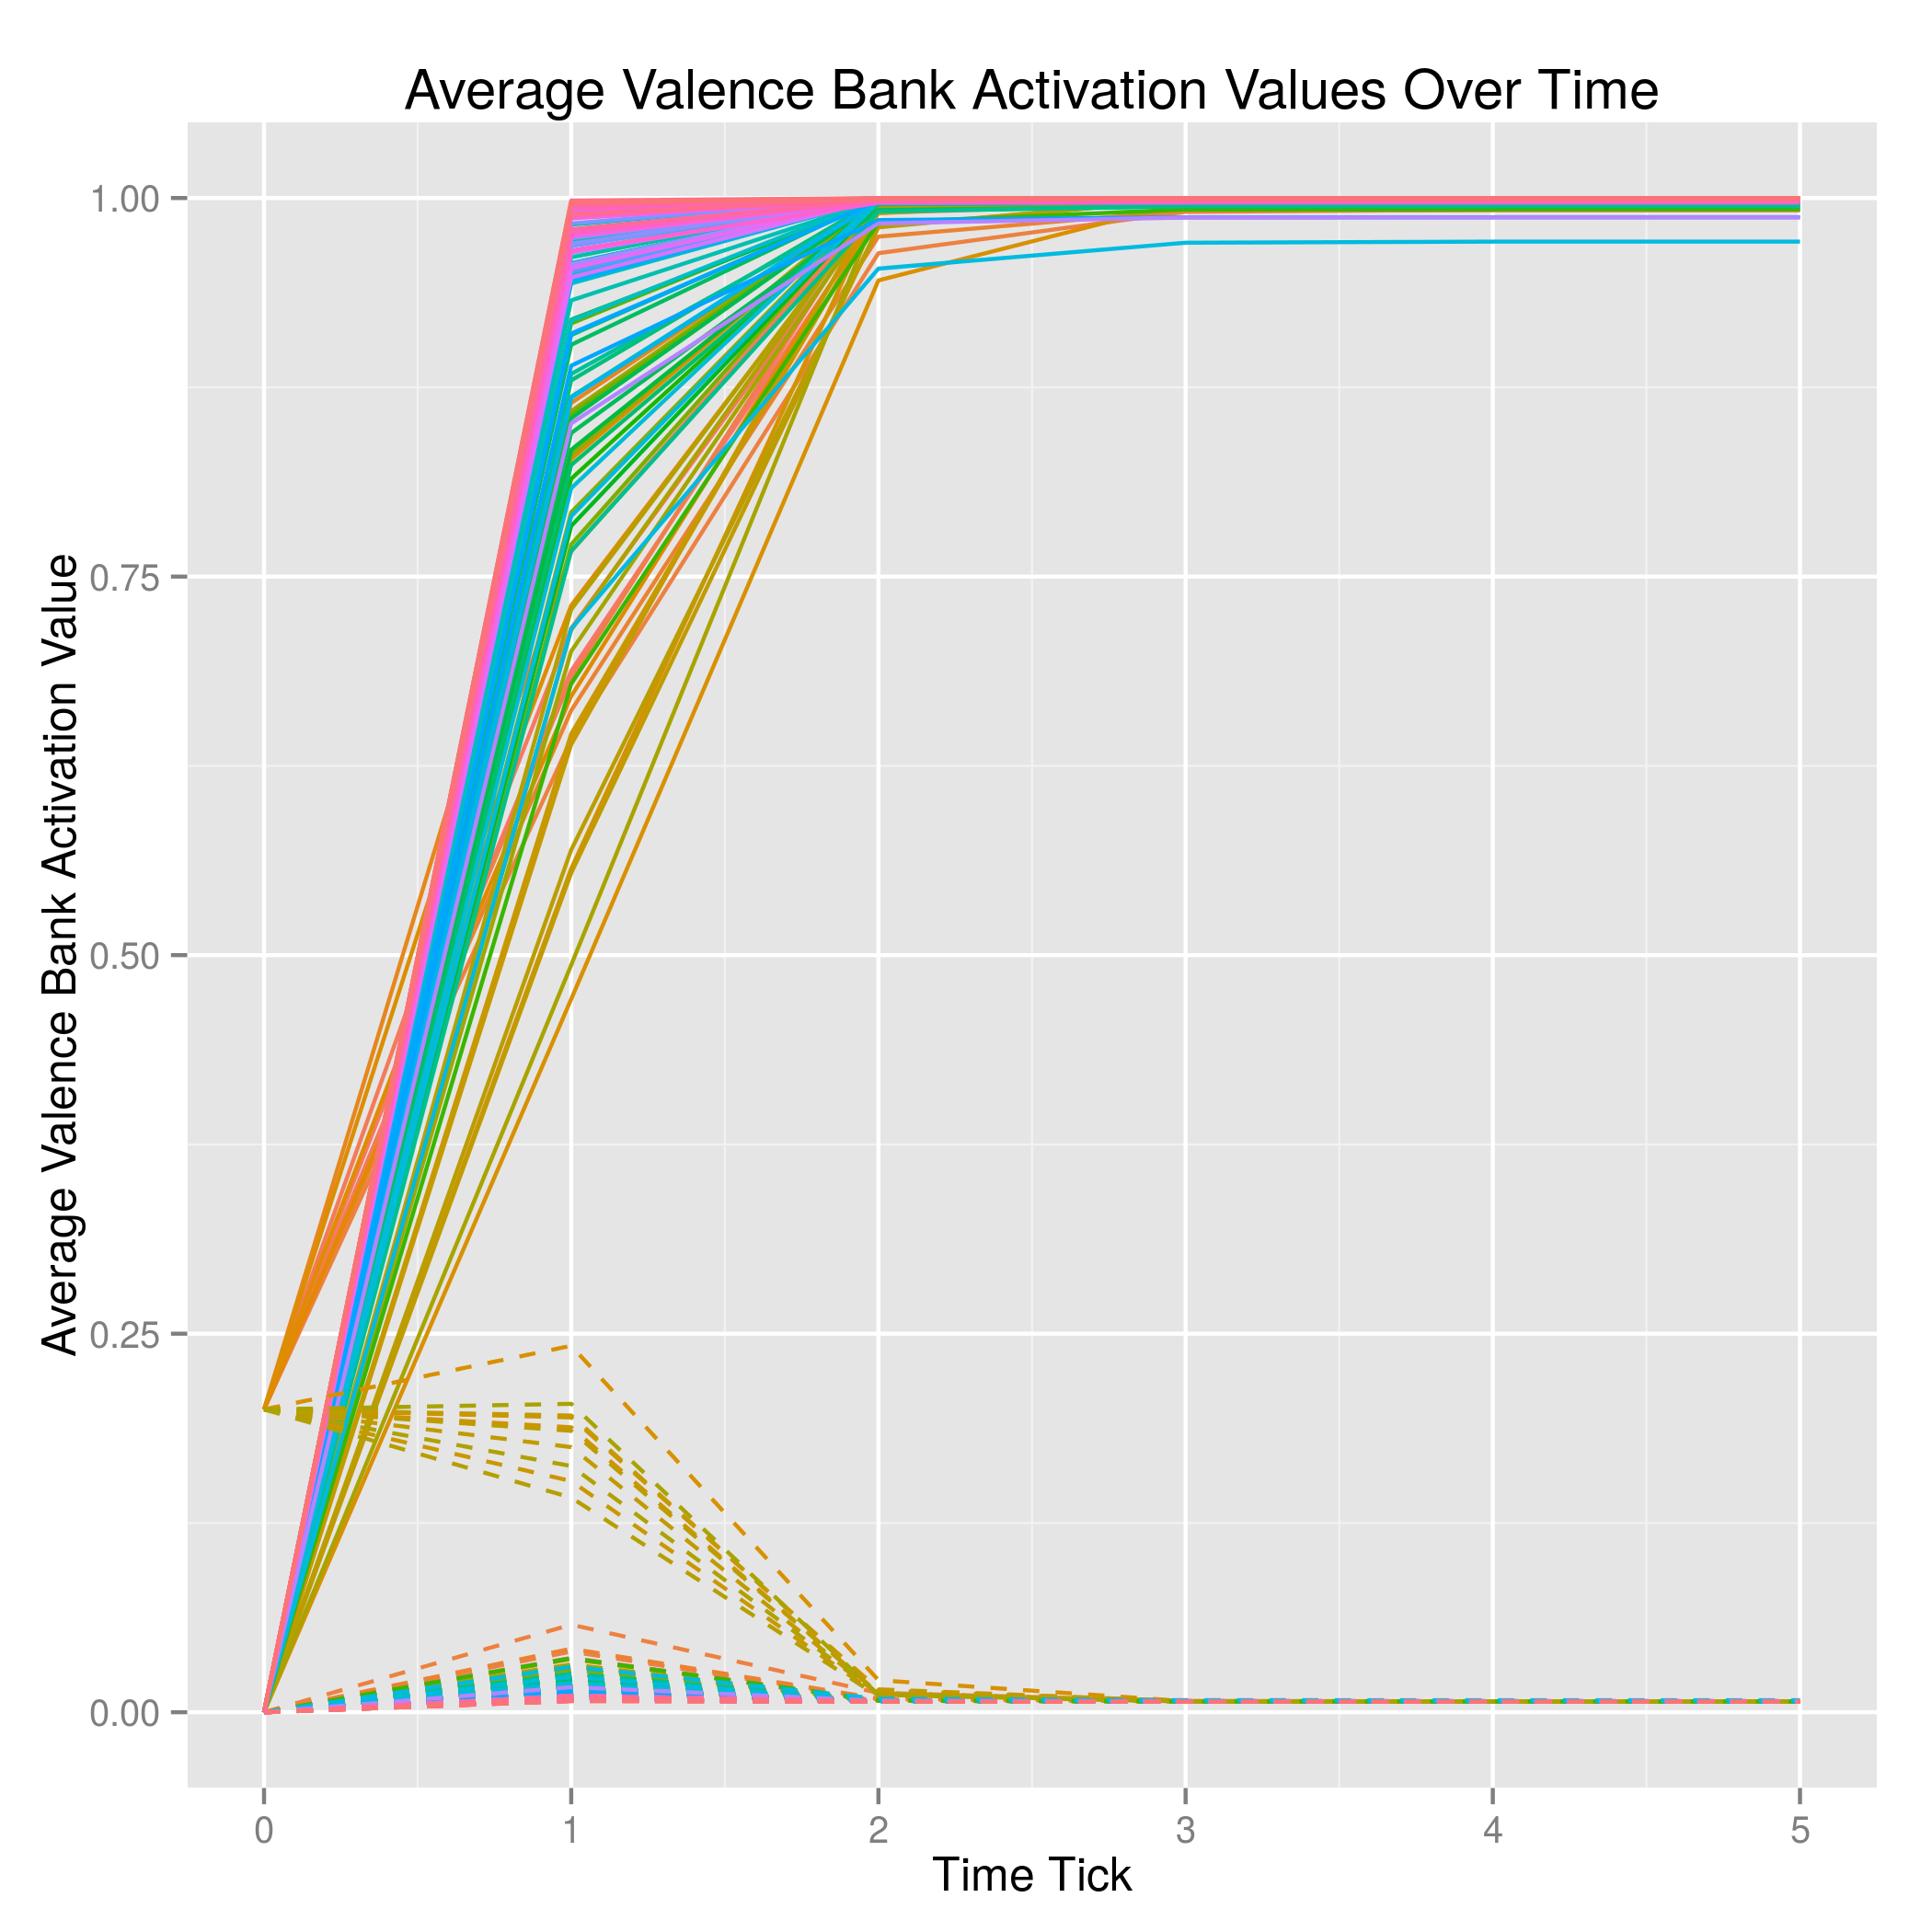
\includegraphics[width=\maxwidth]{figure/unnamed-chunk-15} 
\begin{kframe}

{\ttfamily\noindent\color{warningcolor}{\#\# Warning: Removed 9400 rows containing missing values (geom\_path).\\\#\# Warning: Removed 9400 rows containing missing values (geom\_path).}}\begin{verbatim}
## [1] 7
## [1] 60001
\end{verbatim}


{\ttfamily\noindent\itshape\color{messagecolor}{\#\# Scale for 'x' is already present. Adding another scale for 'x', which will replace the existing scale.}}\end{kframe}
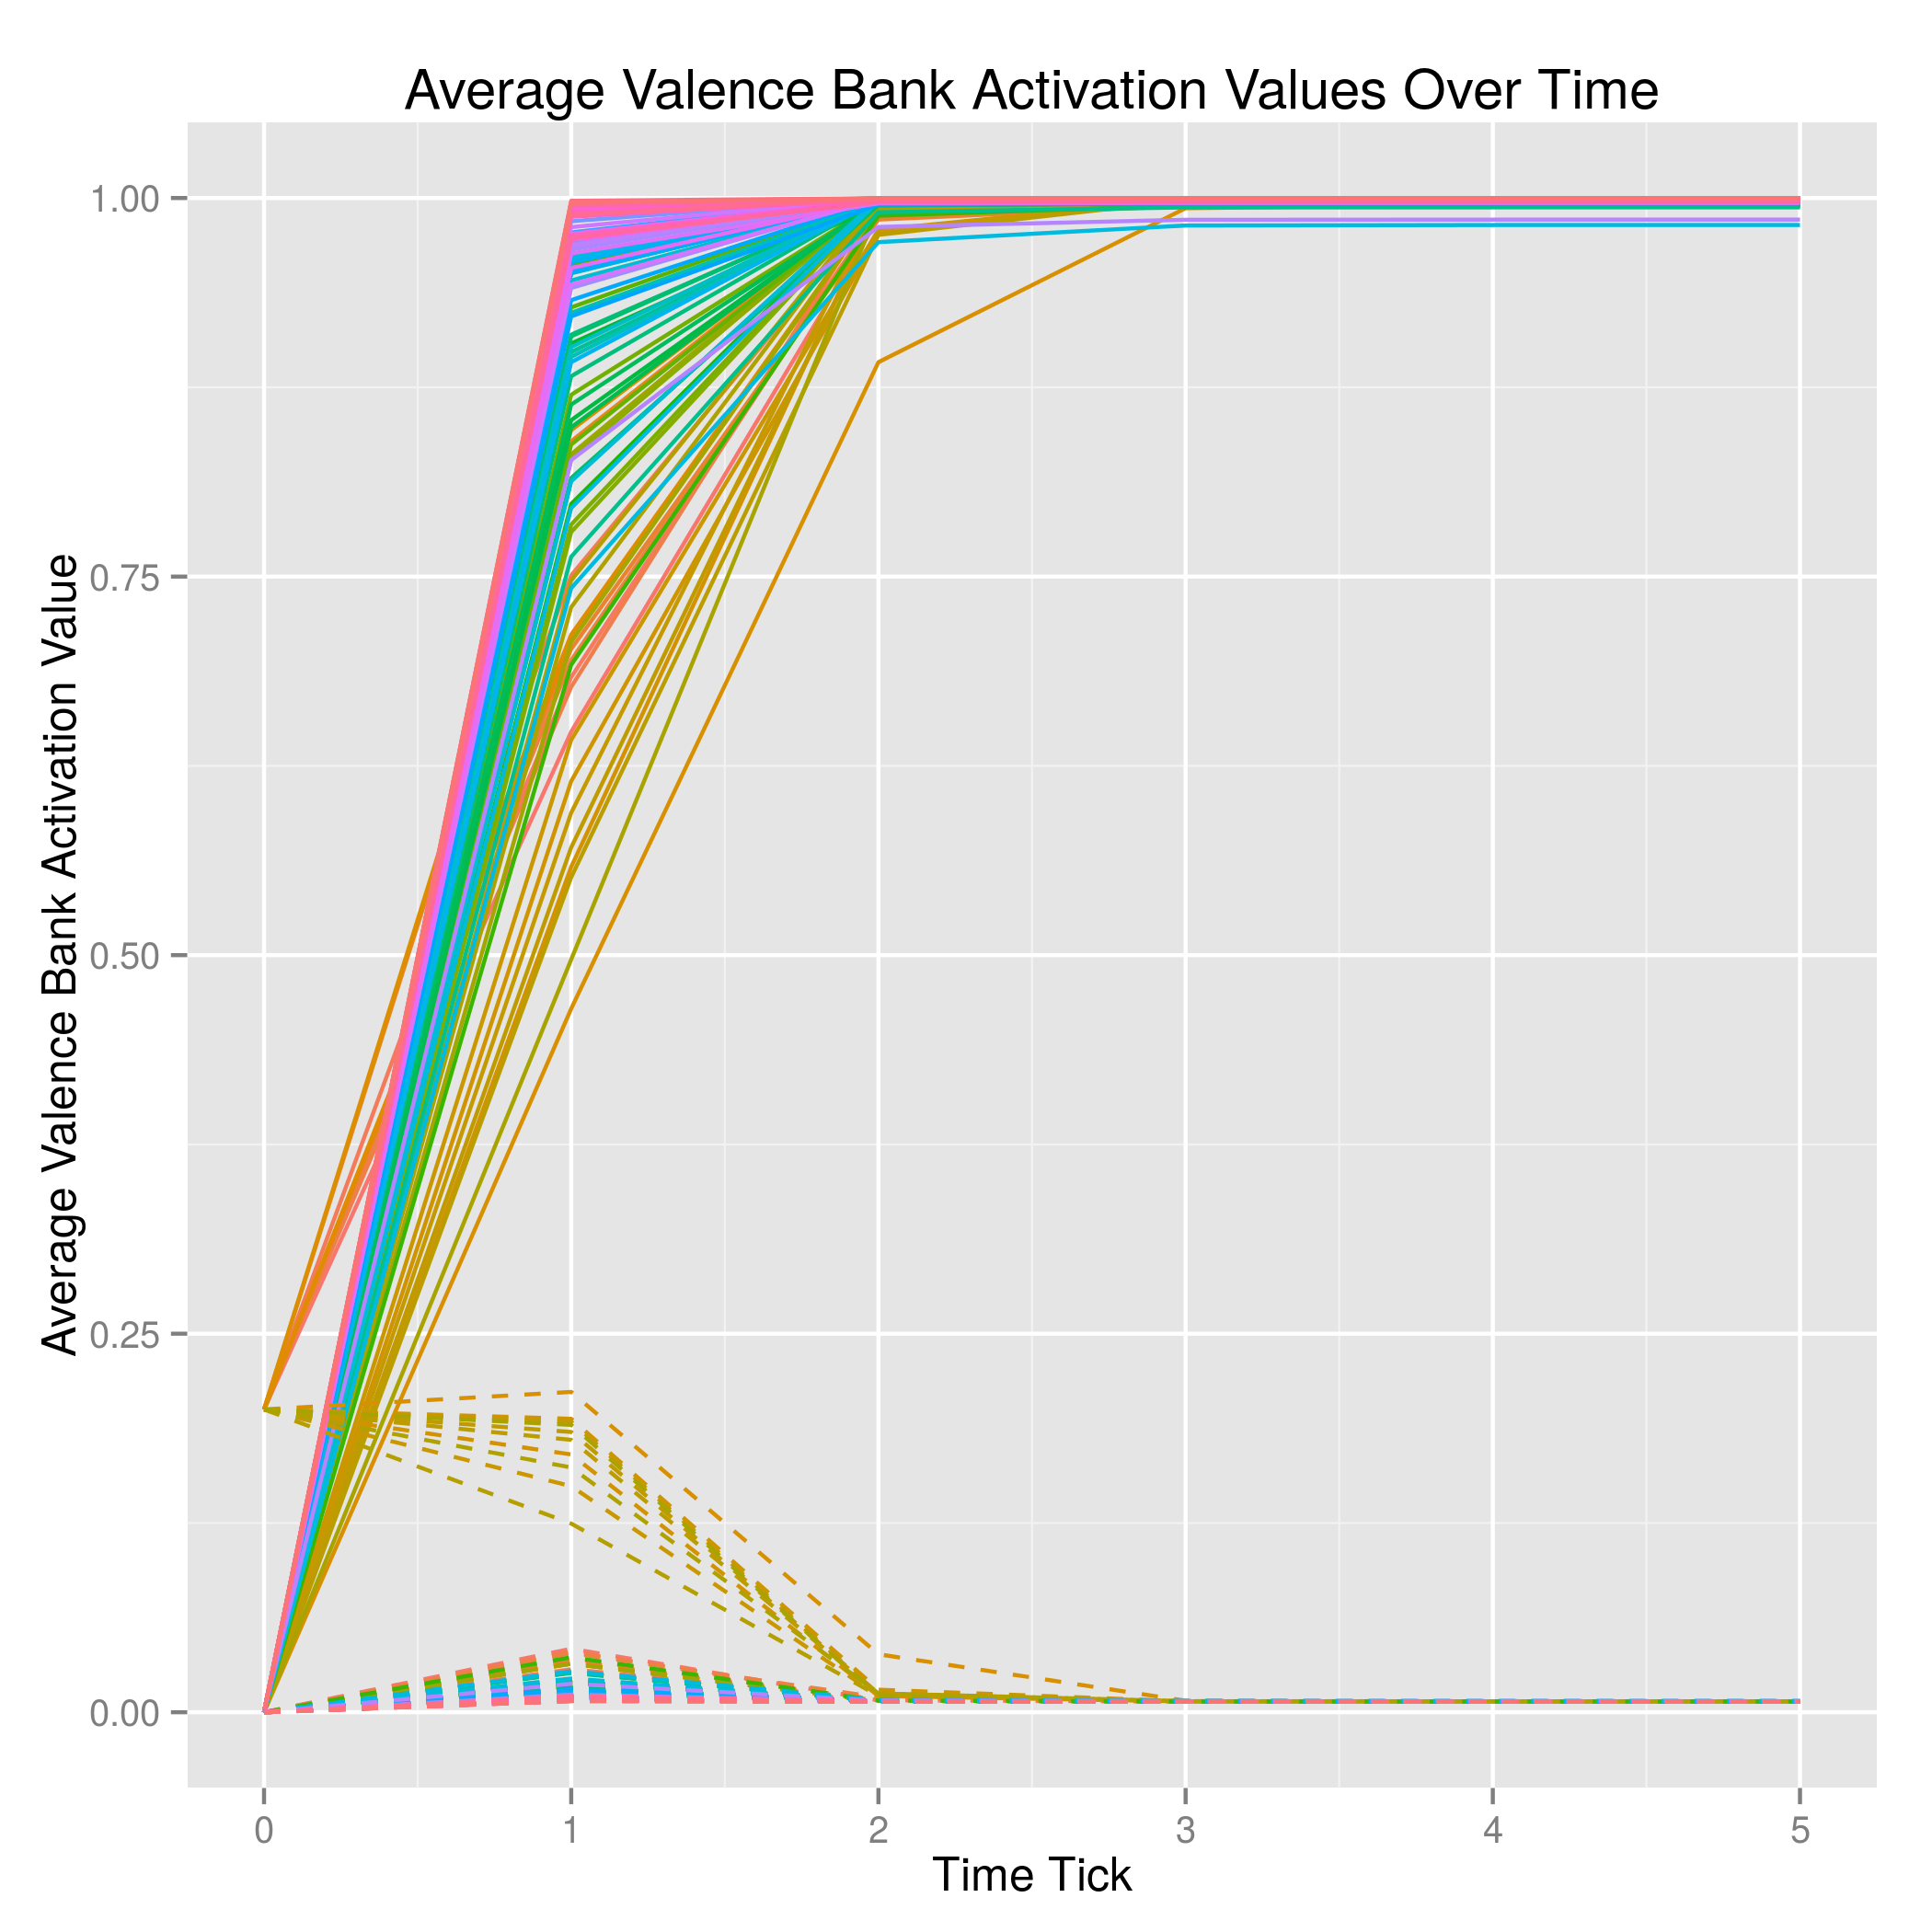
\includegraphics[width=\maxwidth]{figure/unnamed-chunk-16} 
\begin{kframe}

{\ttfamily\noindent\color{warningcolor}{\#\# Warning: Removed 9400 rows containing missing values (geom\_path).\\\#\# Warning: Removed 9400 rows containing missing values (geom\_path).}}\begin{verbatim}
## [1] 8
## [1] 70001
\end{verbatim}


{\ttfamily\noindent\itshape\color{messagecolor}{\#\# Scale for 'x' is already present. Adding another scale for 'x', which will replace the existing scale.}}\end{kframe}
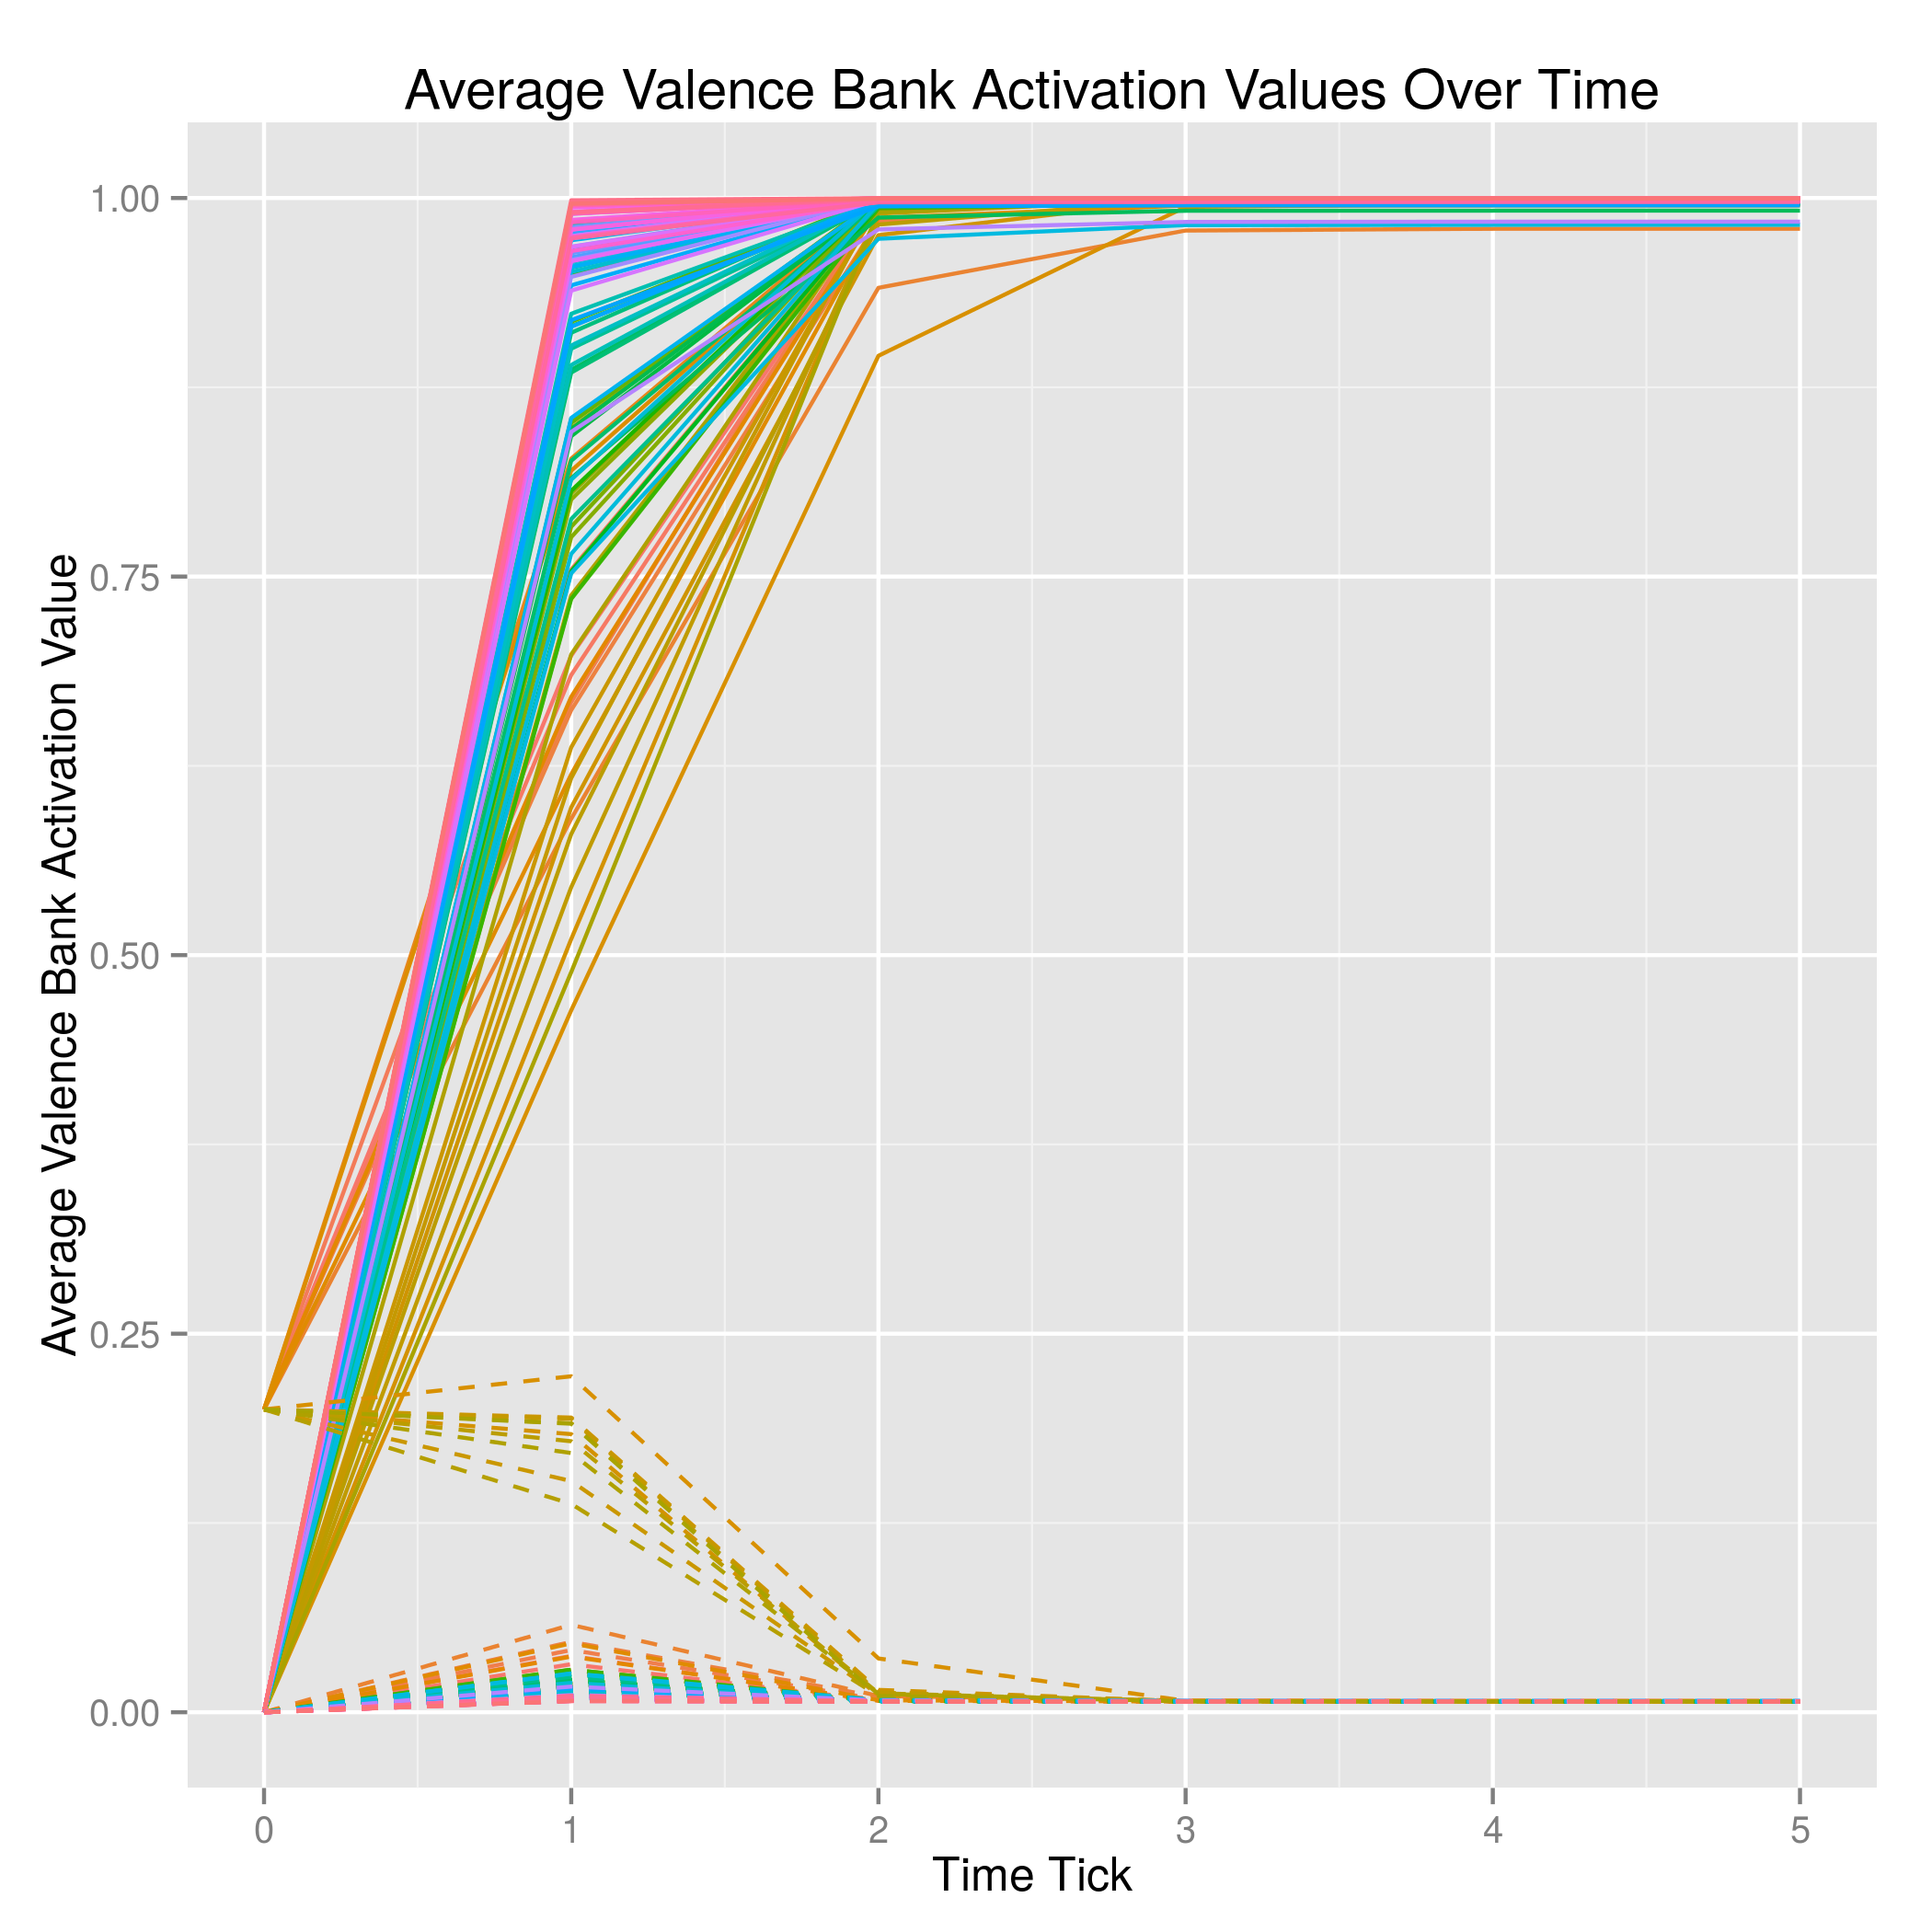
\includegraphics[width=\maxwidth]{figure/unnamed-chunk-17} 
\begin{kframe}

{\ttfamily\noindent\color{warningcolor}{\#\# Warning: Removed 9400 rows containing missing values (geom\_path).\\\#\# Warning: Removed 9400 rows containing missing values (geom\_path).}}\begin{verbatim}
## [1] 9
## [1] 80001
\end{verbatim}


{\ttfamily\noindent\itshape\color{messagecolor}{\#\# Scale for 'x' is already present. Adding another scale for 'x', which will replace the existing scale.}}\end{kframe}
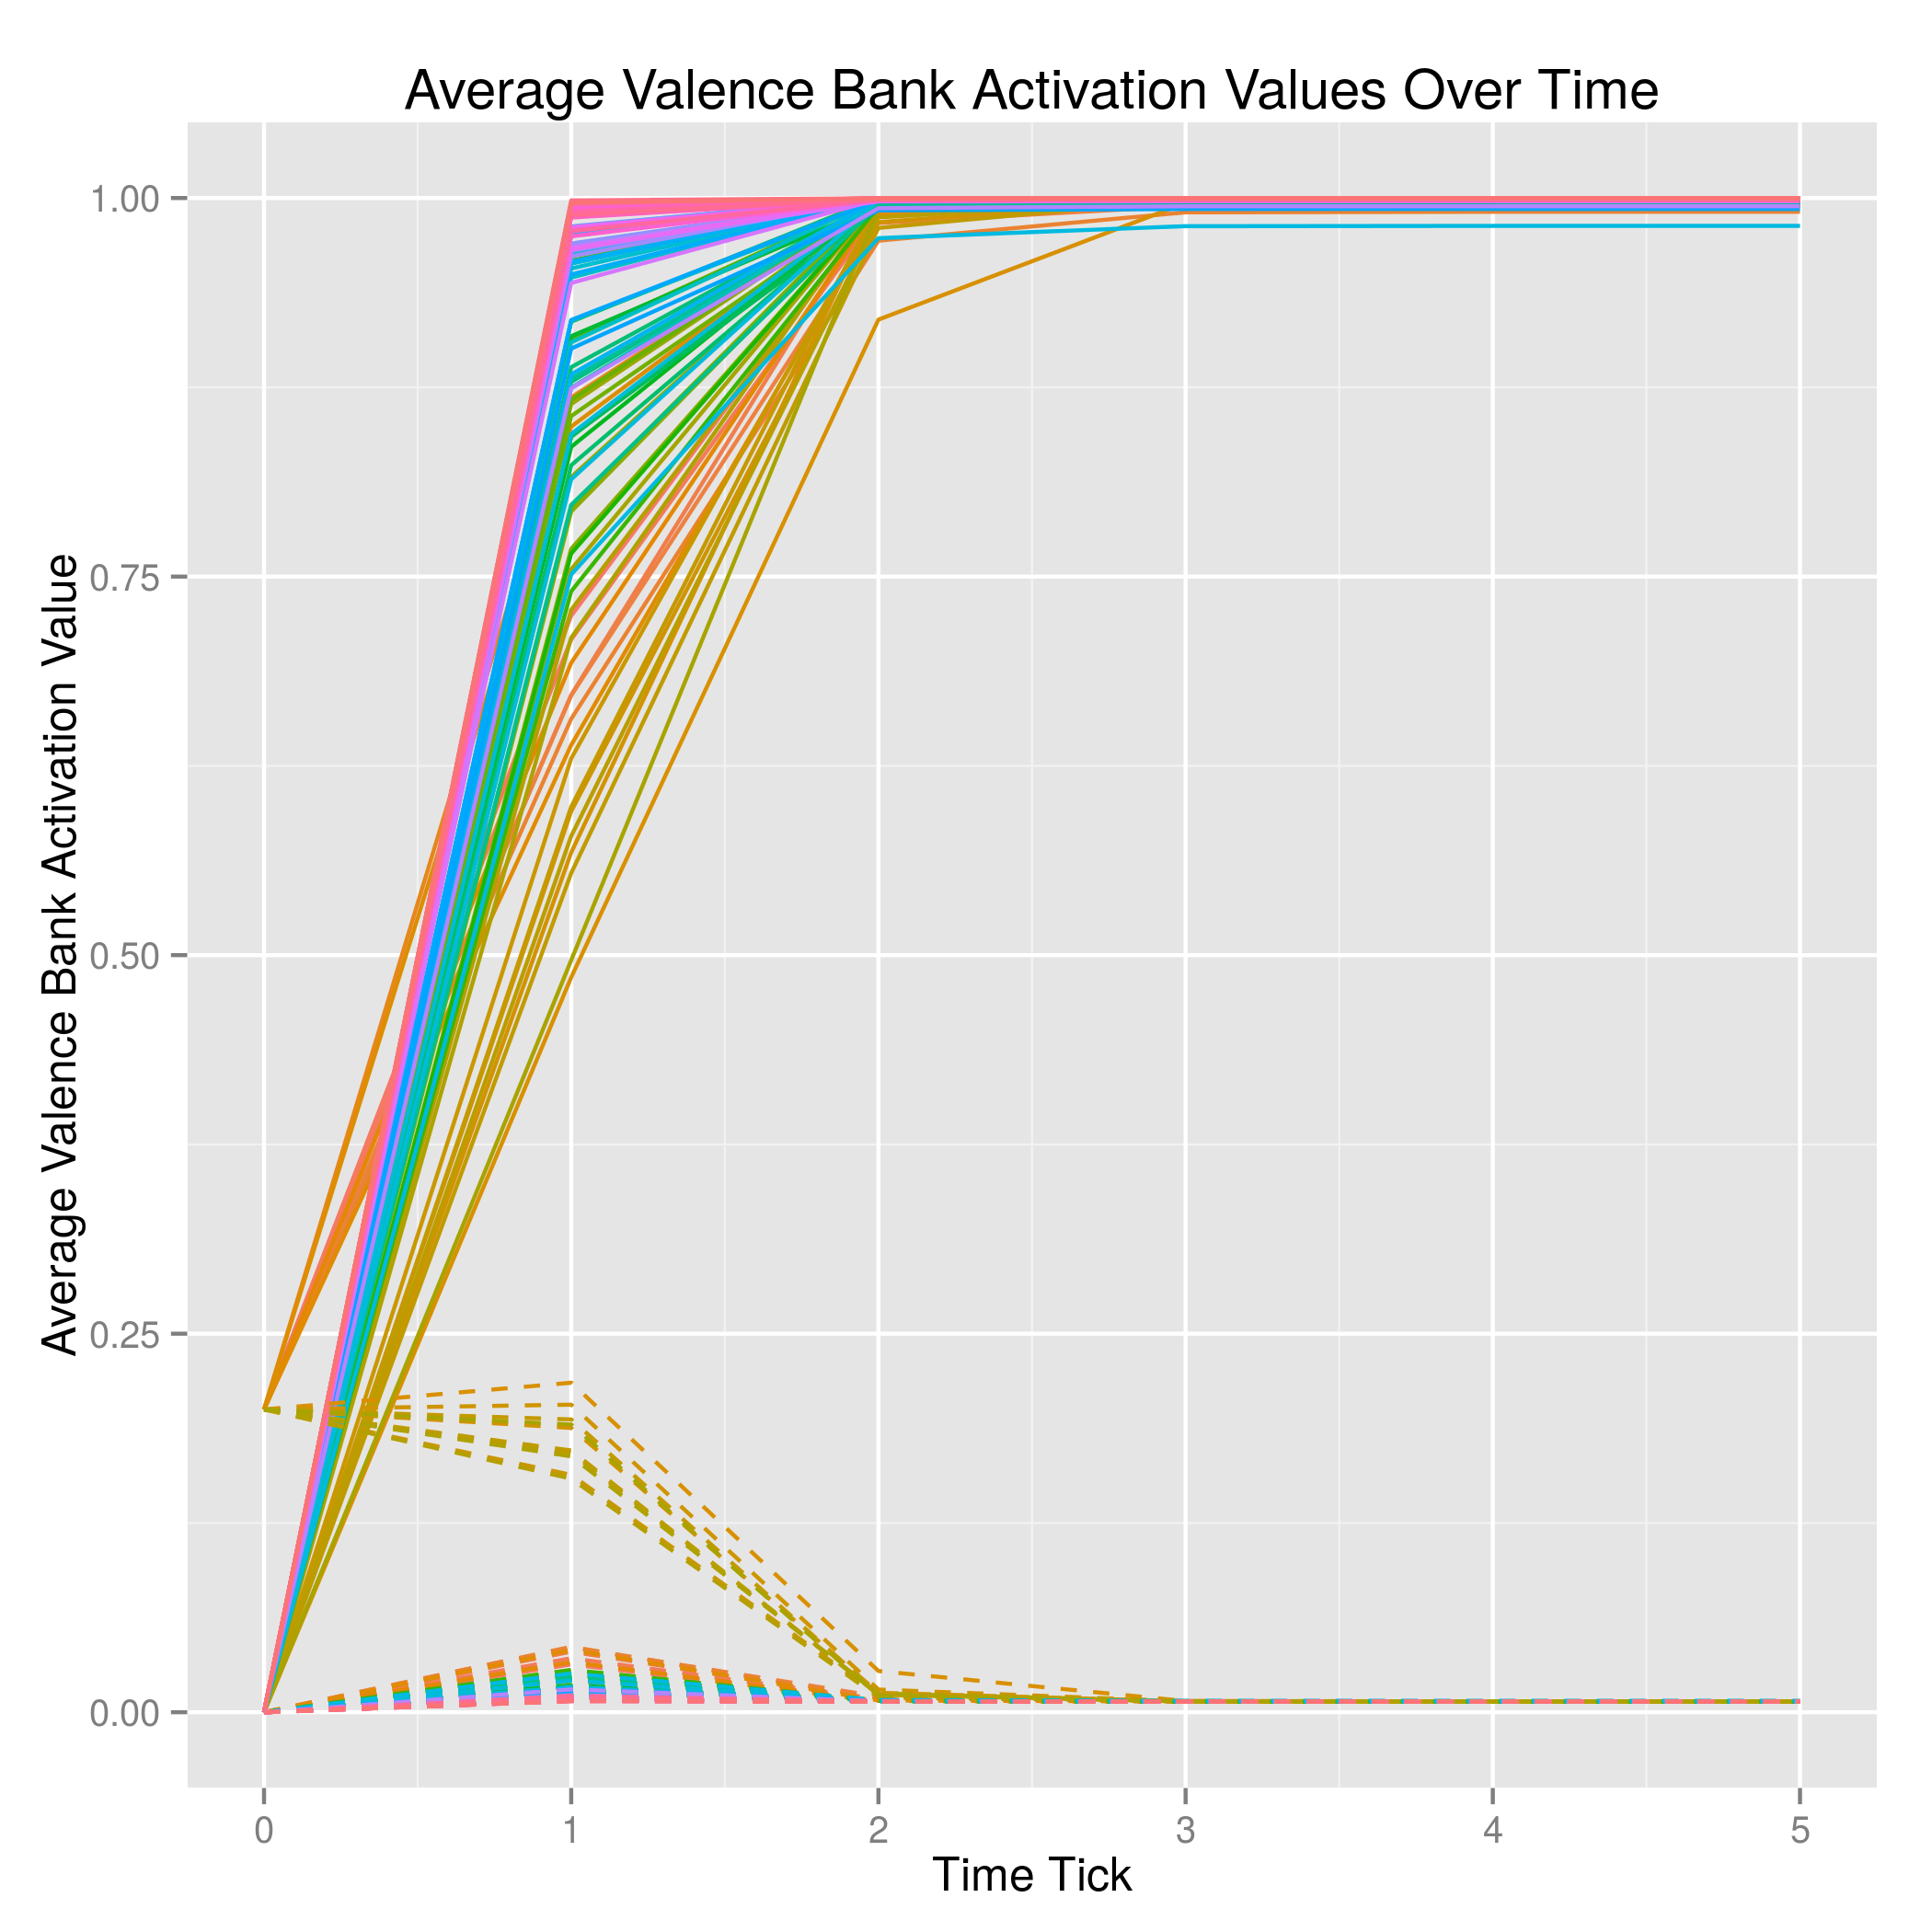
\includegraphics[width=\maxwidth]{figure/unnamed-chunk-18} 
\begin{kframe}

{\ttfamily\noindent\color{warningcolor}{\#\# Warning: Removed 9400 rows containing missing values (geom\_path).\\\#\# Warning: Removed 9400 rows containing missing values (geom\_path).}}\begin{verbatim}
## [1] 10
## [1] 90001
\end{verbatim}


{\ttfamily\noindent\itshape\color{messagecolor}{\#\# Scale for 'x' is already present. Adding another scale for 'x', which will replace the existing scale.}}\end{kframe}
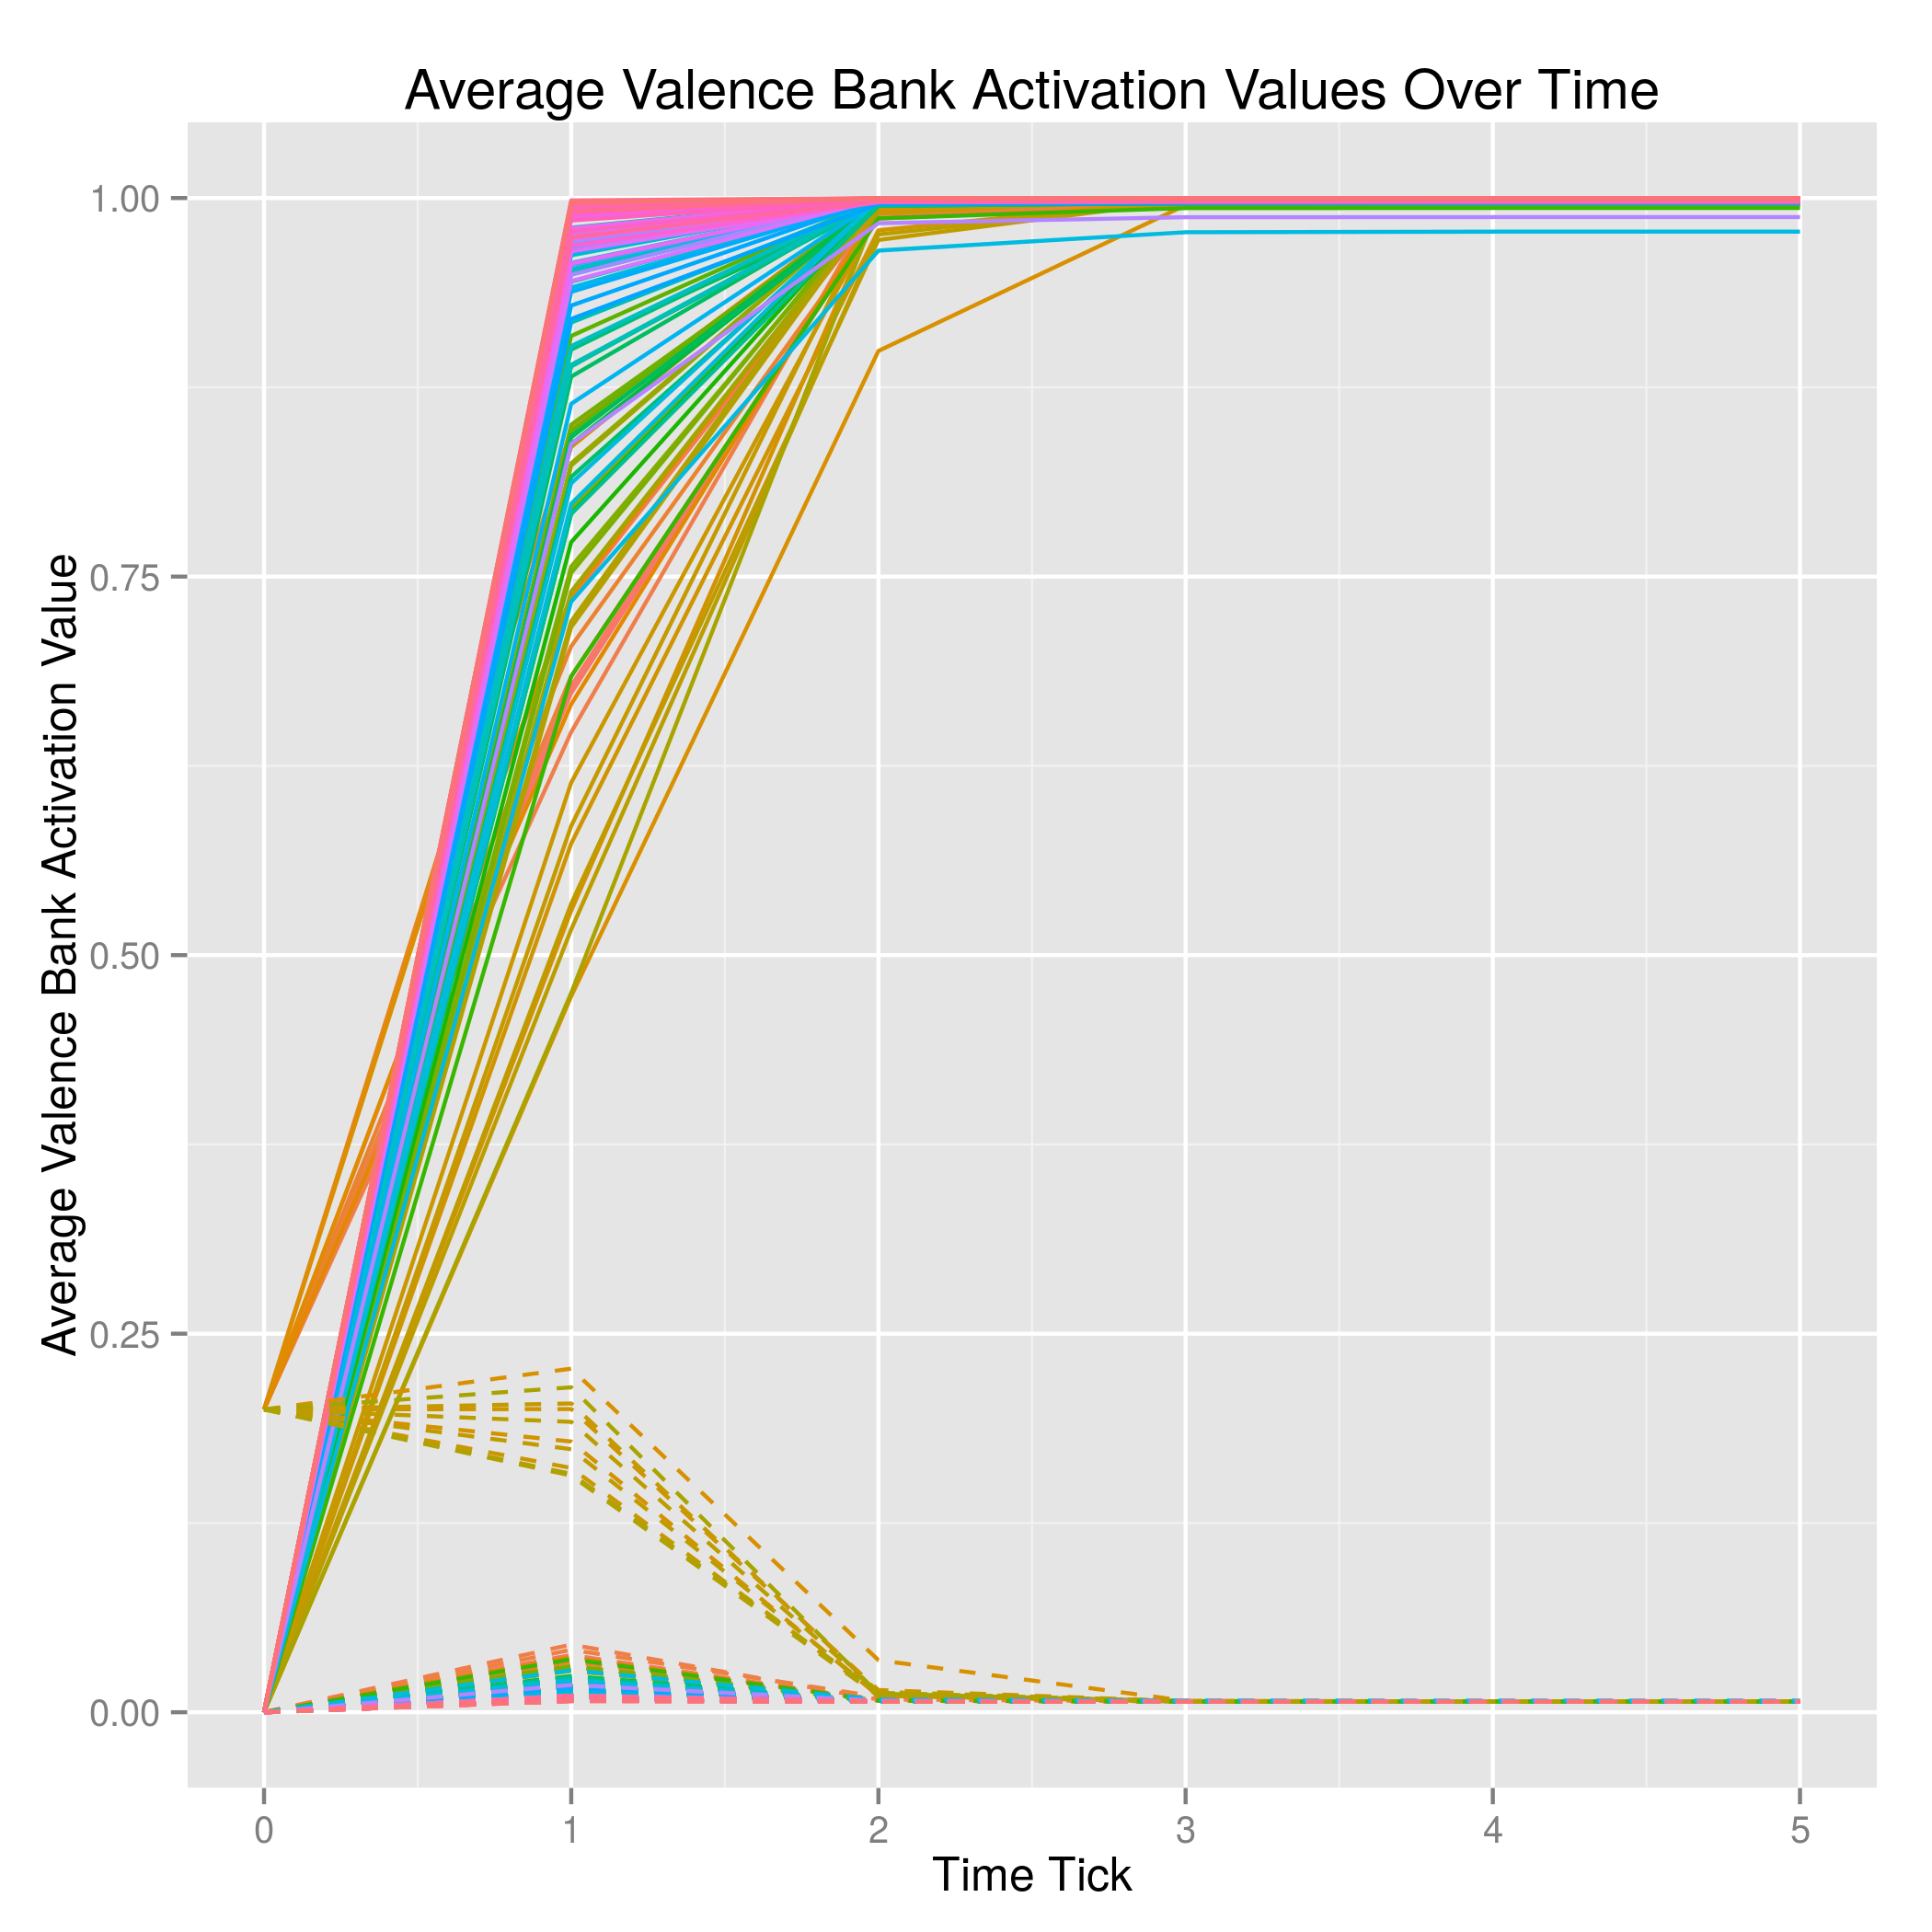
\includegraphics[width=\maxwidth]{figure/unnamed-chunk-19} 
\begin{kframe}

{\ttfamily\noindent\color{warningcolor}{\#\# Warning: Removed 9400 rows containing missing values (geom\_path).\\\#\# Warning: Removed 9400 rows containing missing values (geom\_path).}}\end{kframe}
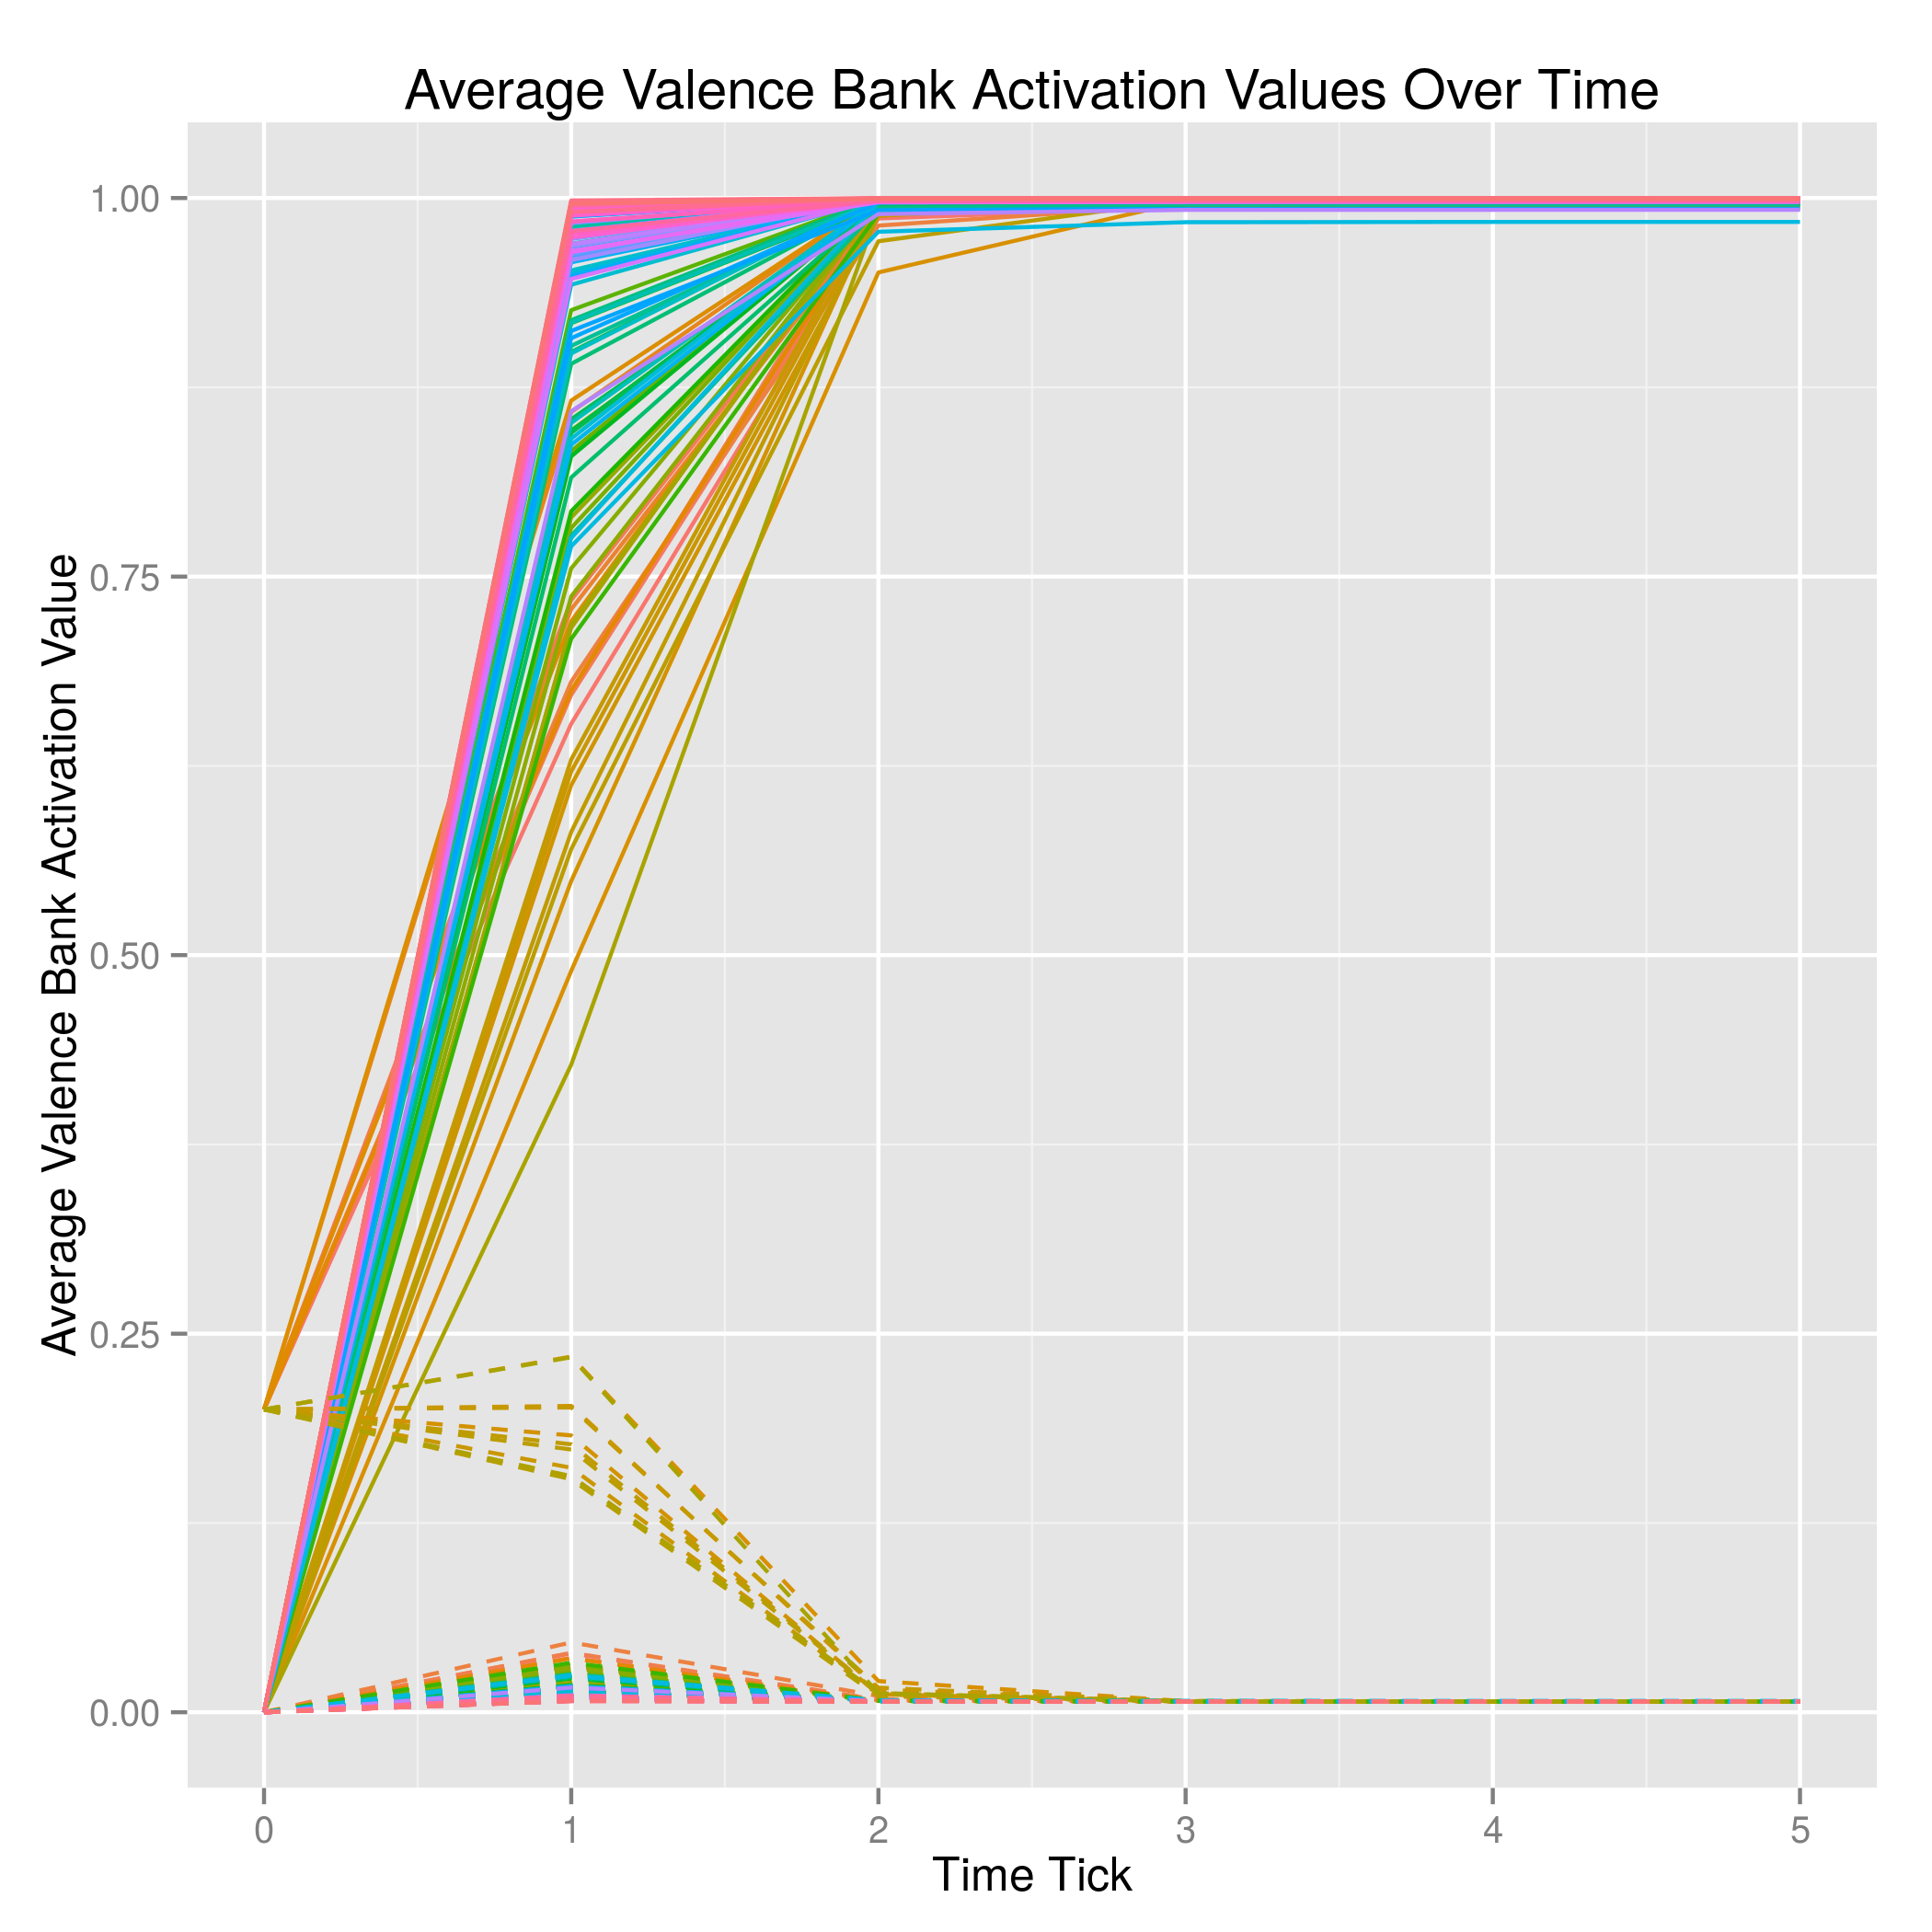
\includegraphics[width=\maxwidth]{figure/unnamed-chunk-110} 

\end{knitrout}


\newpage
\subsubsection{All time ticks}
\begin{knitrout}
\definecolor{shadecolor}{rgb}{0.969, 0.969, 0.969}\color{fgcolor}\begin{kframe}
\begin{alltt}
\hlkwd{source}\hlstd{(}\hlkwc{file} \hlstd{=} \hlstr{"../plot-function-ggplot2.R"}\hlstd{)}
\hlkwd{plot.multiple.run.data}\hlstd{(}\hlstr{"../data/exp/exp1b.csv"}\hlstd{,} \hlnum{100}\hlstd{,} \hlnum{100}\hlstd{)}
\end{alltt}
\begin{verbatim}
## [1] 1
## [1] 1
\end{verbatim}
\end{kframe}
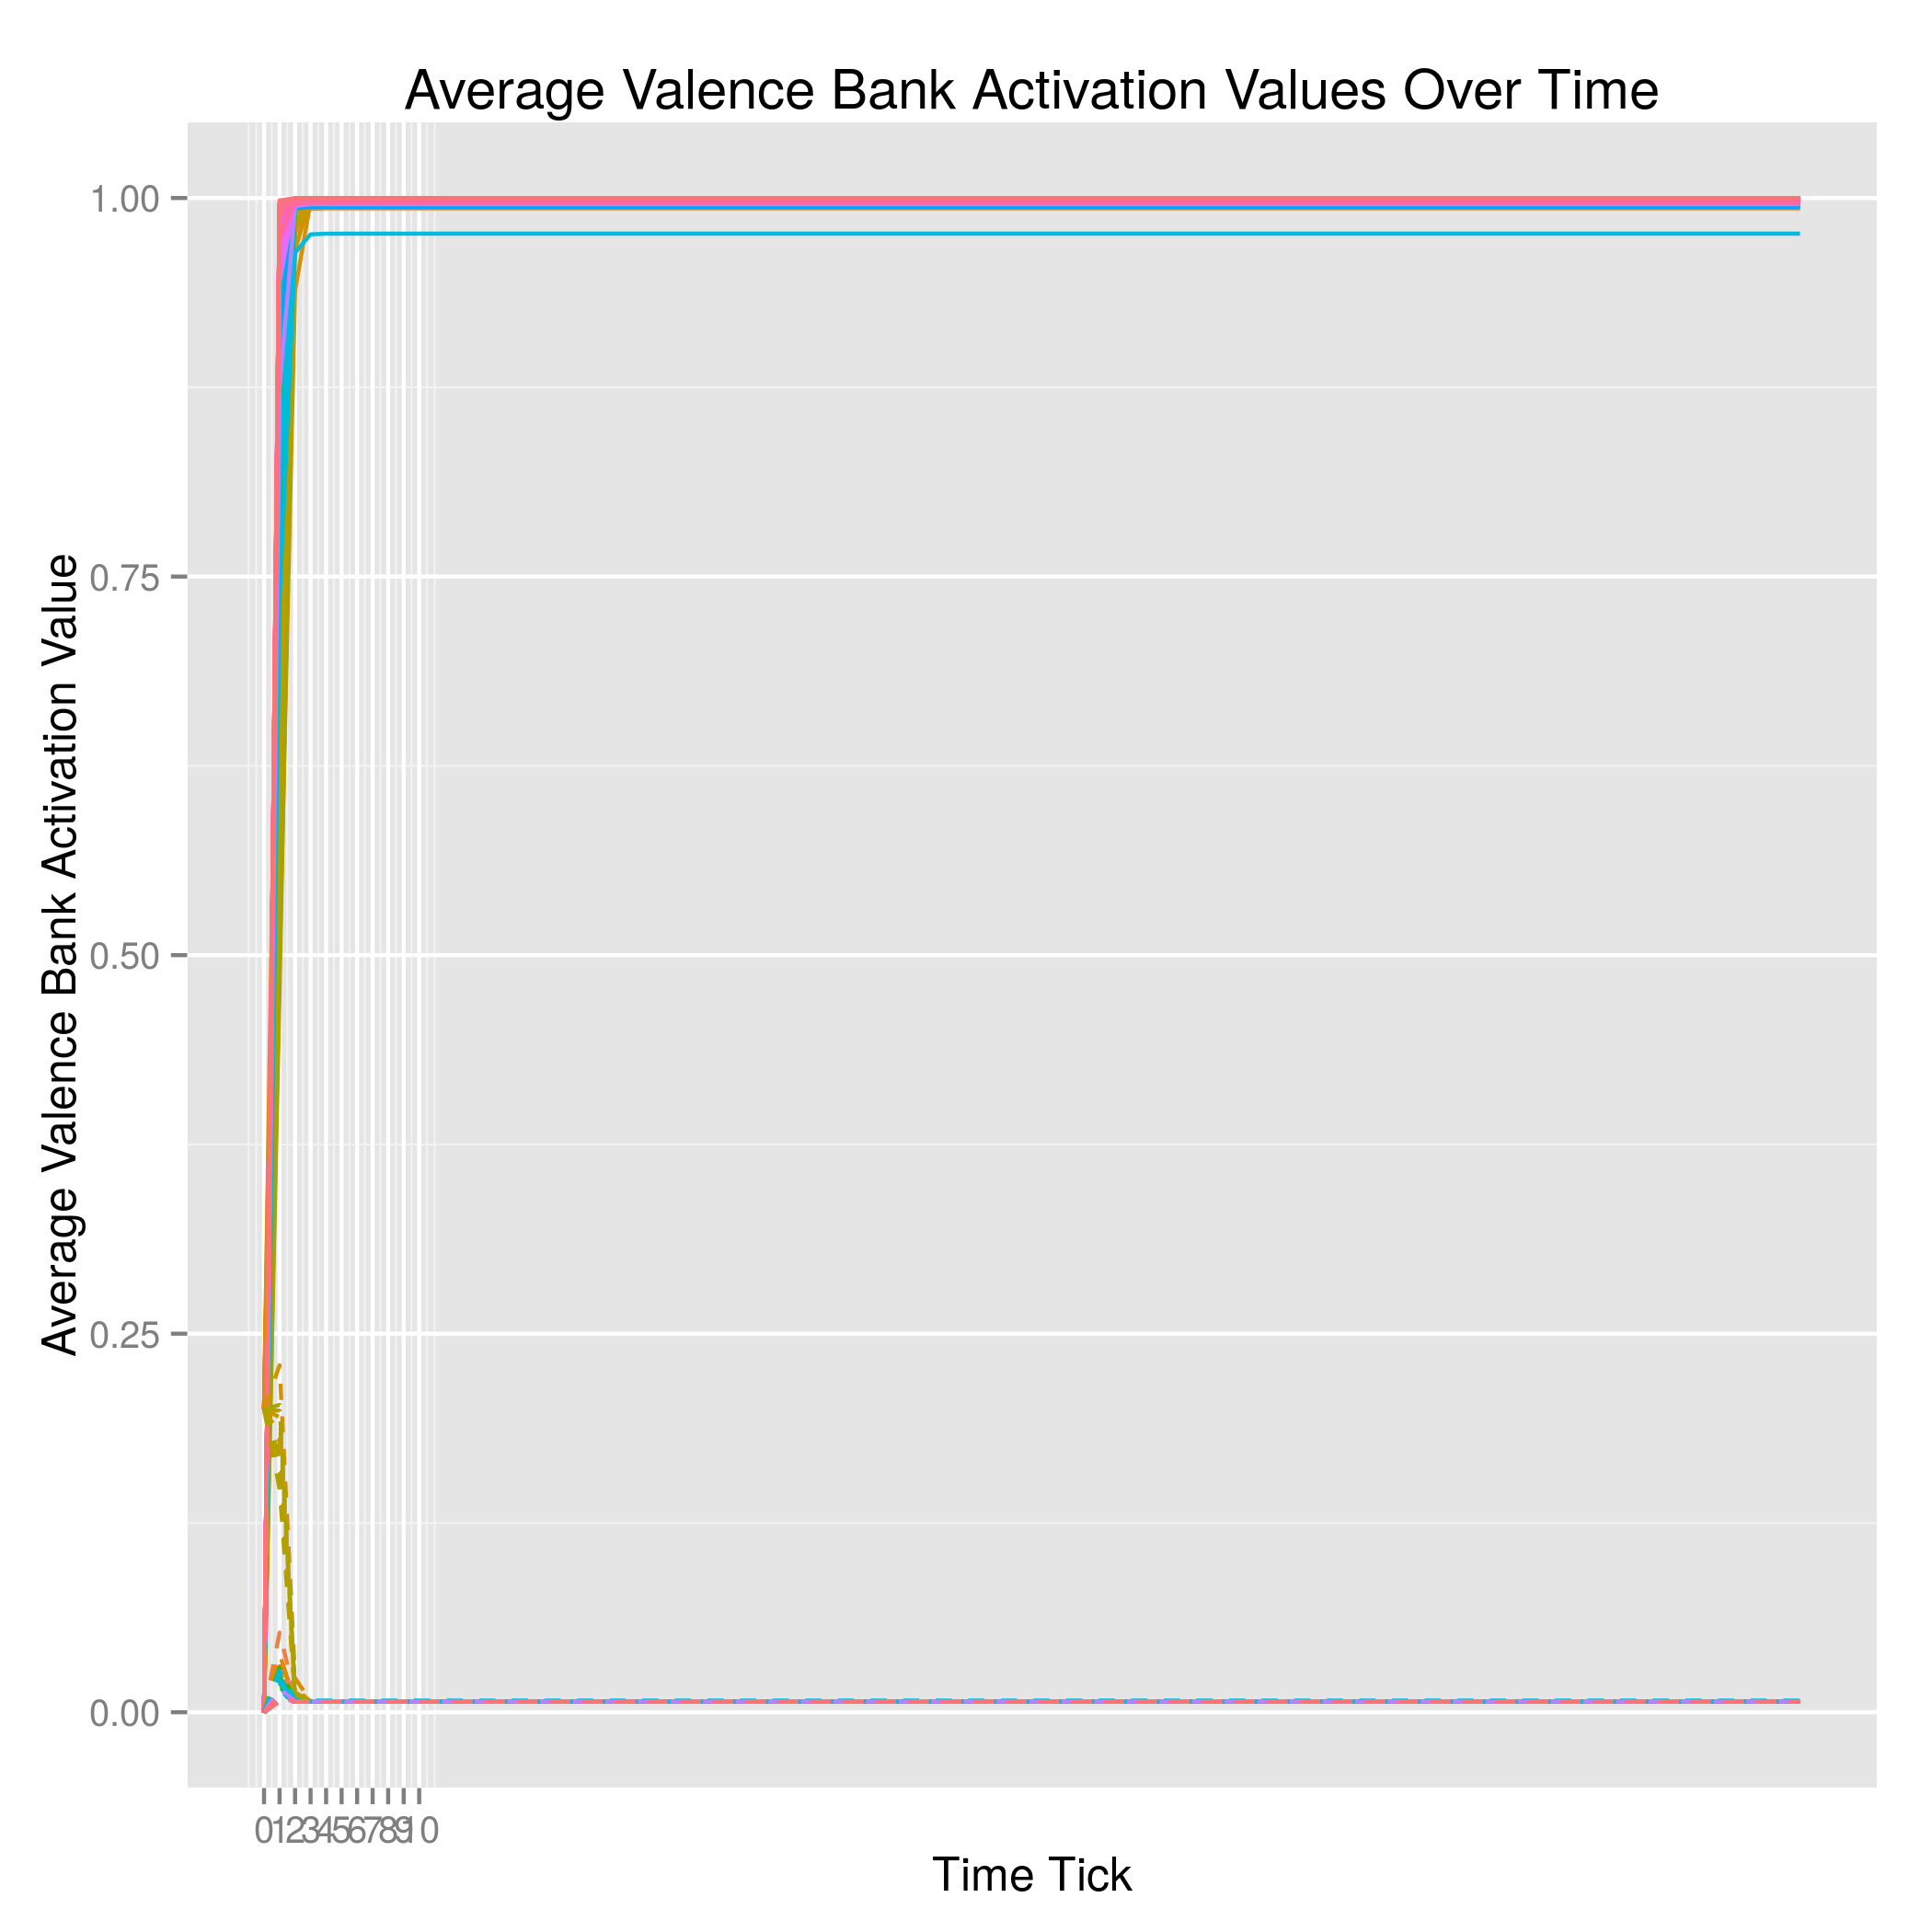
\includegraphics[width=\maxwidth]{figure/unnamed-chunk-21} 
\begin{kframe}\begin{verbatim}
## [1] 2
## [1] 10001
\end{verbatim}
\end{kframe}
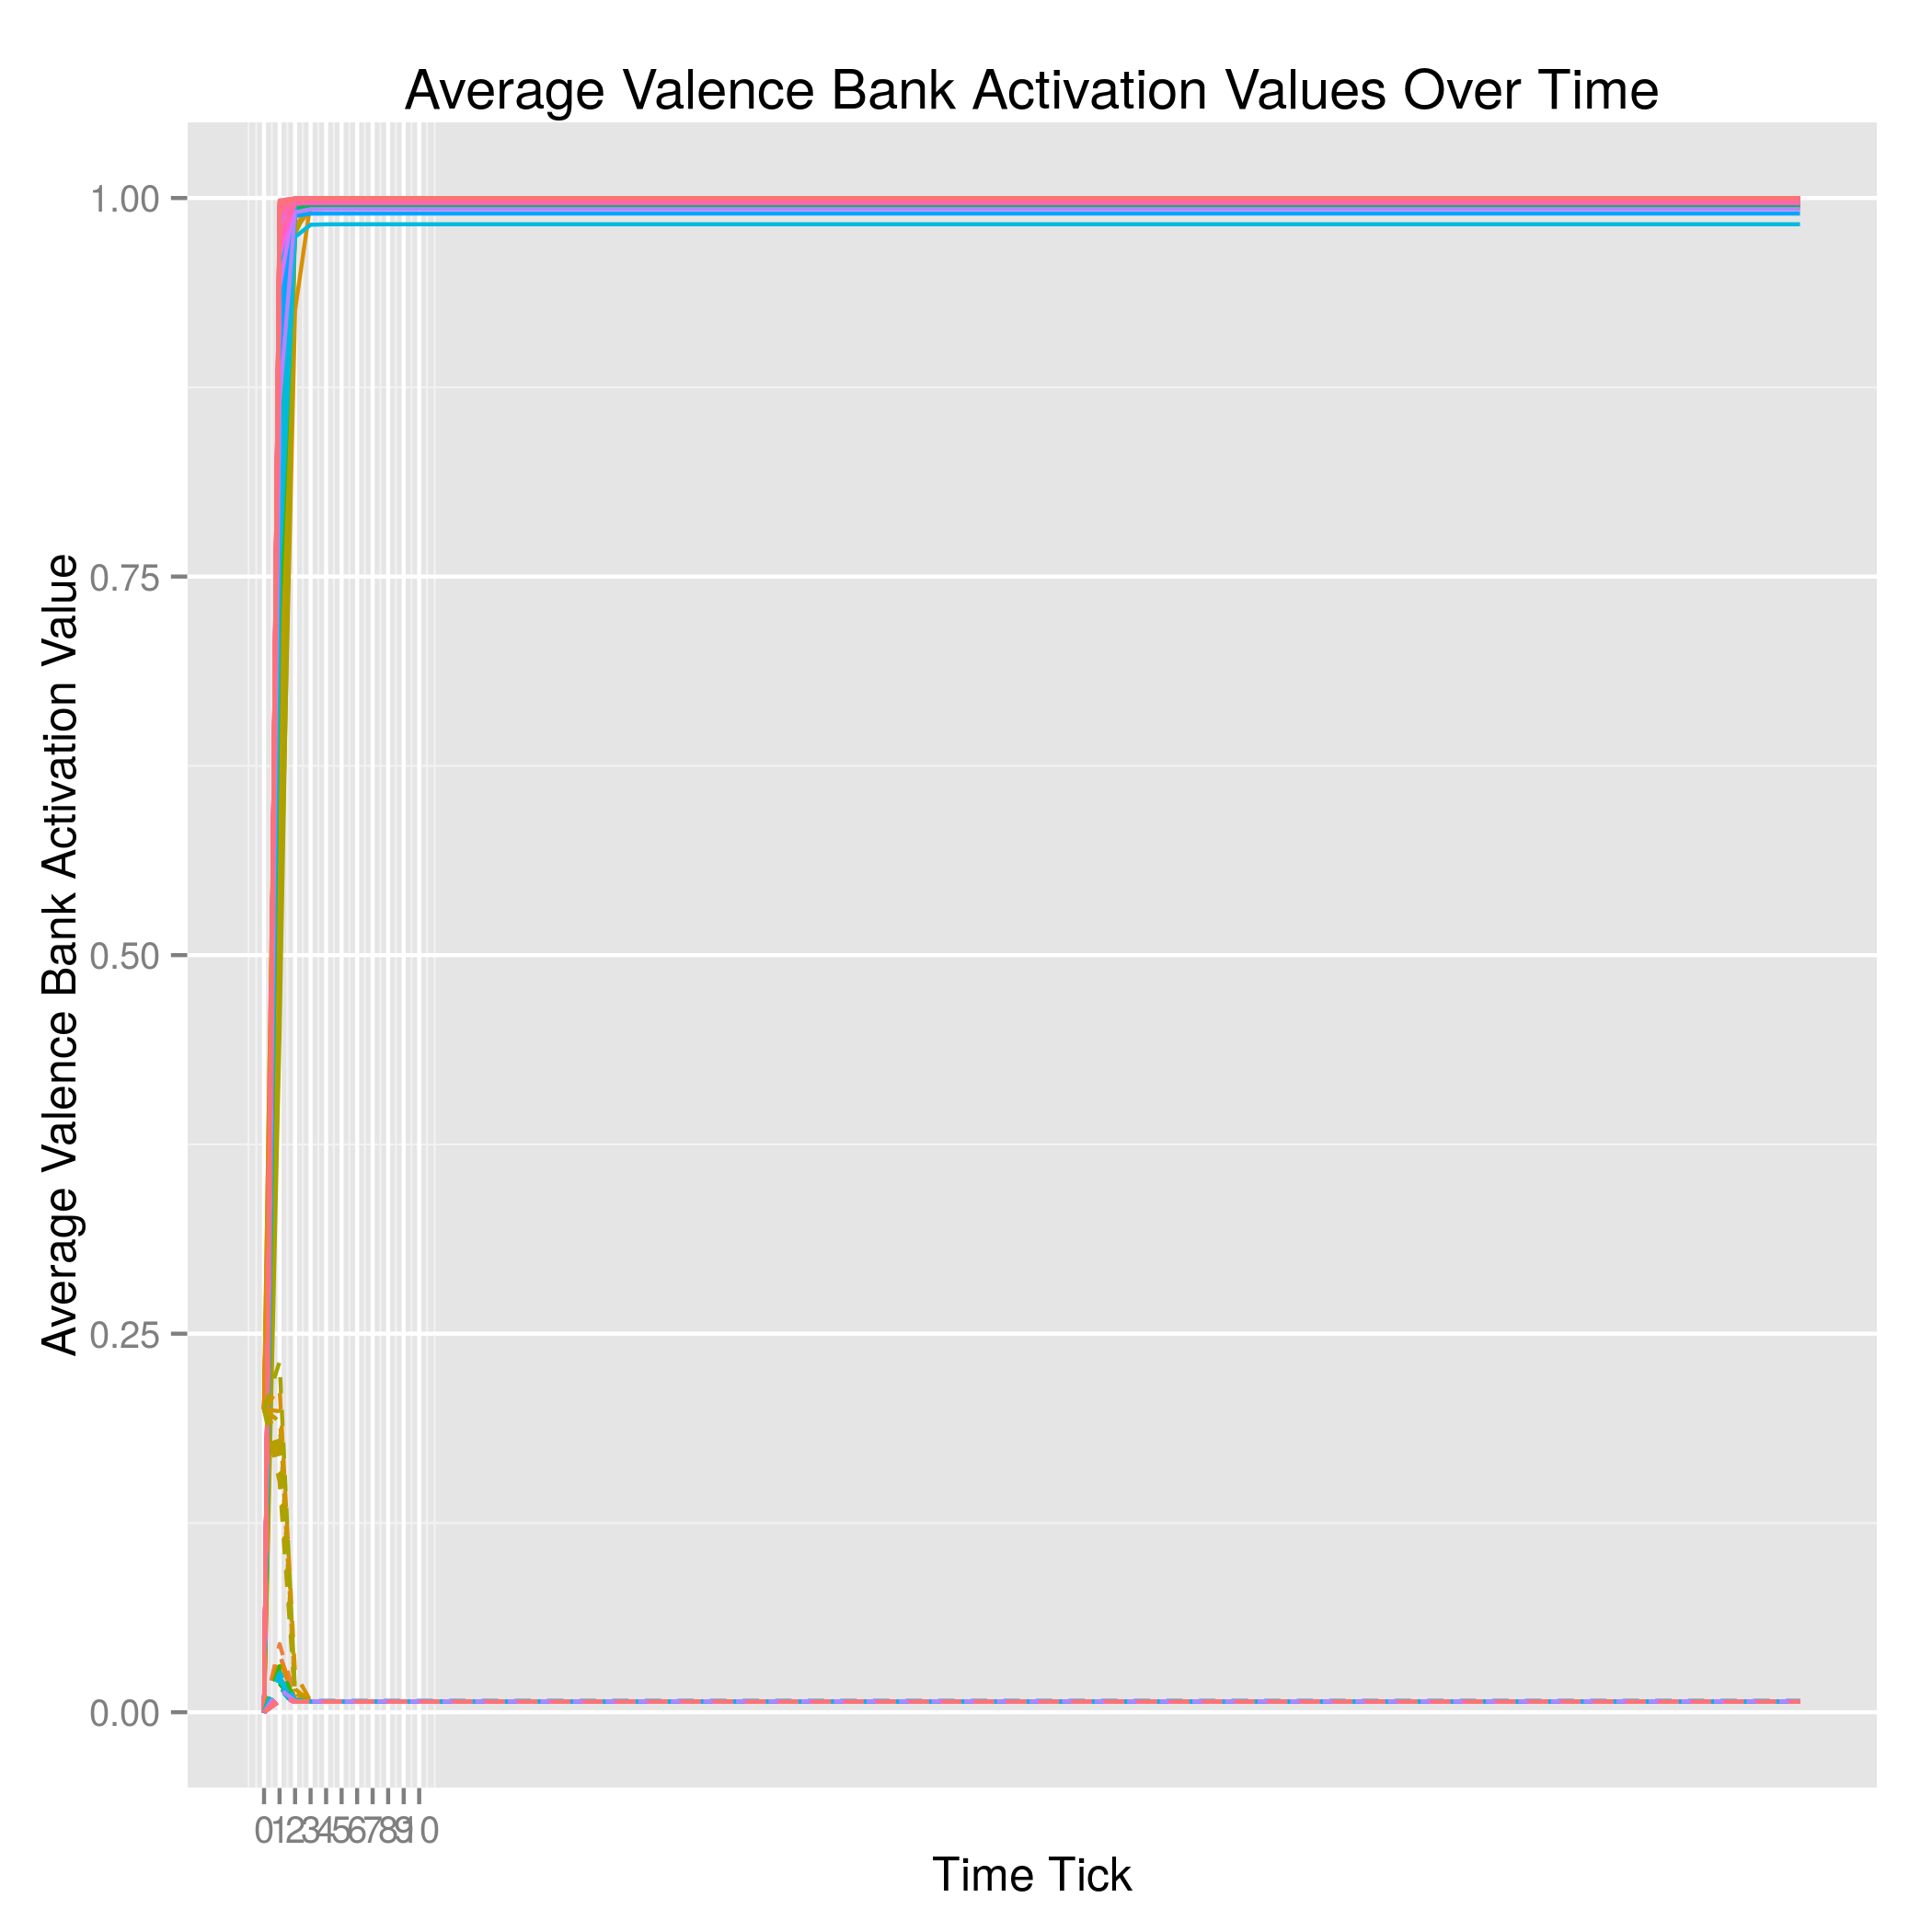
\includegraphics[width=\maxwidth]{figure/unnamed-chunk-22} 
\begin{kframe}\begin{verbatim}
## [1] 3
## [1] 20001
\end{verbatim}
\end{kframe}
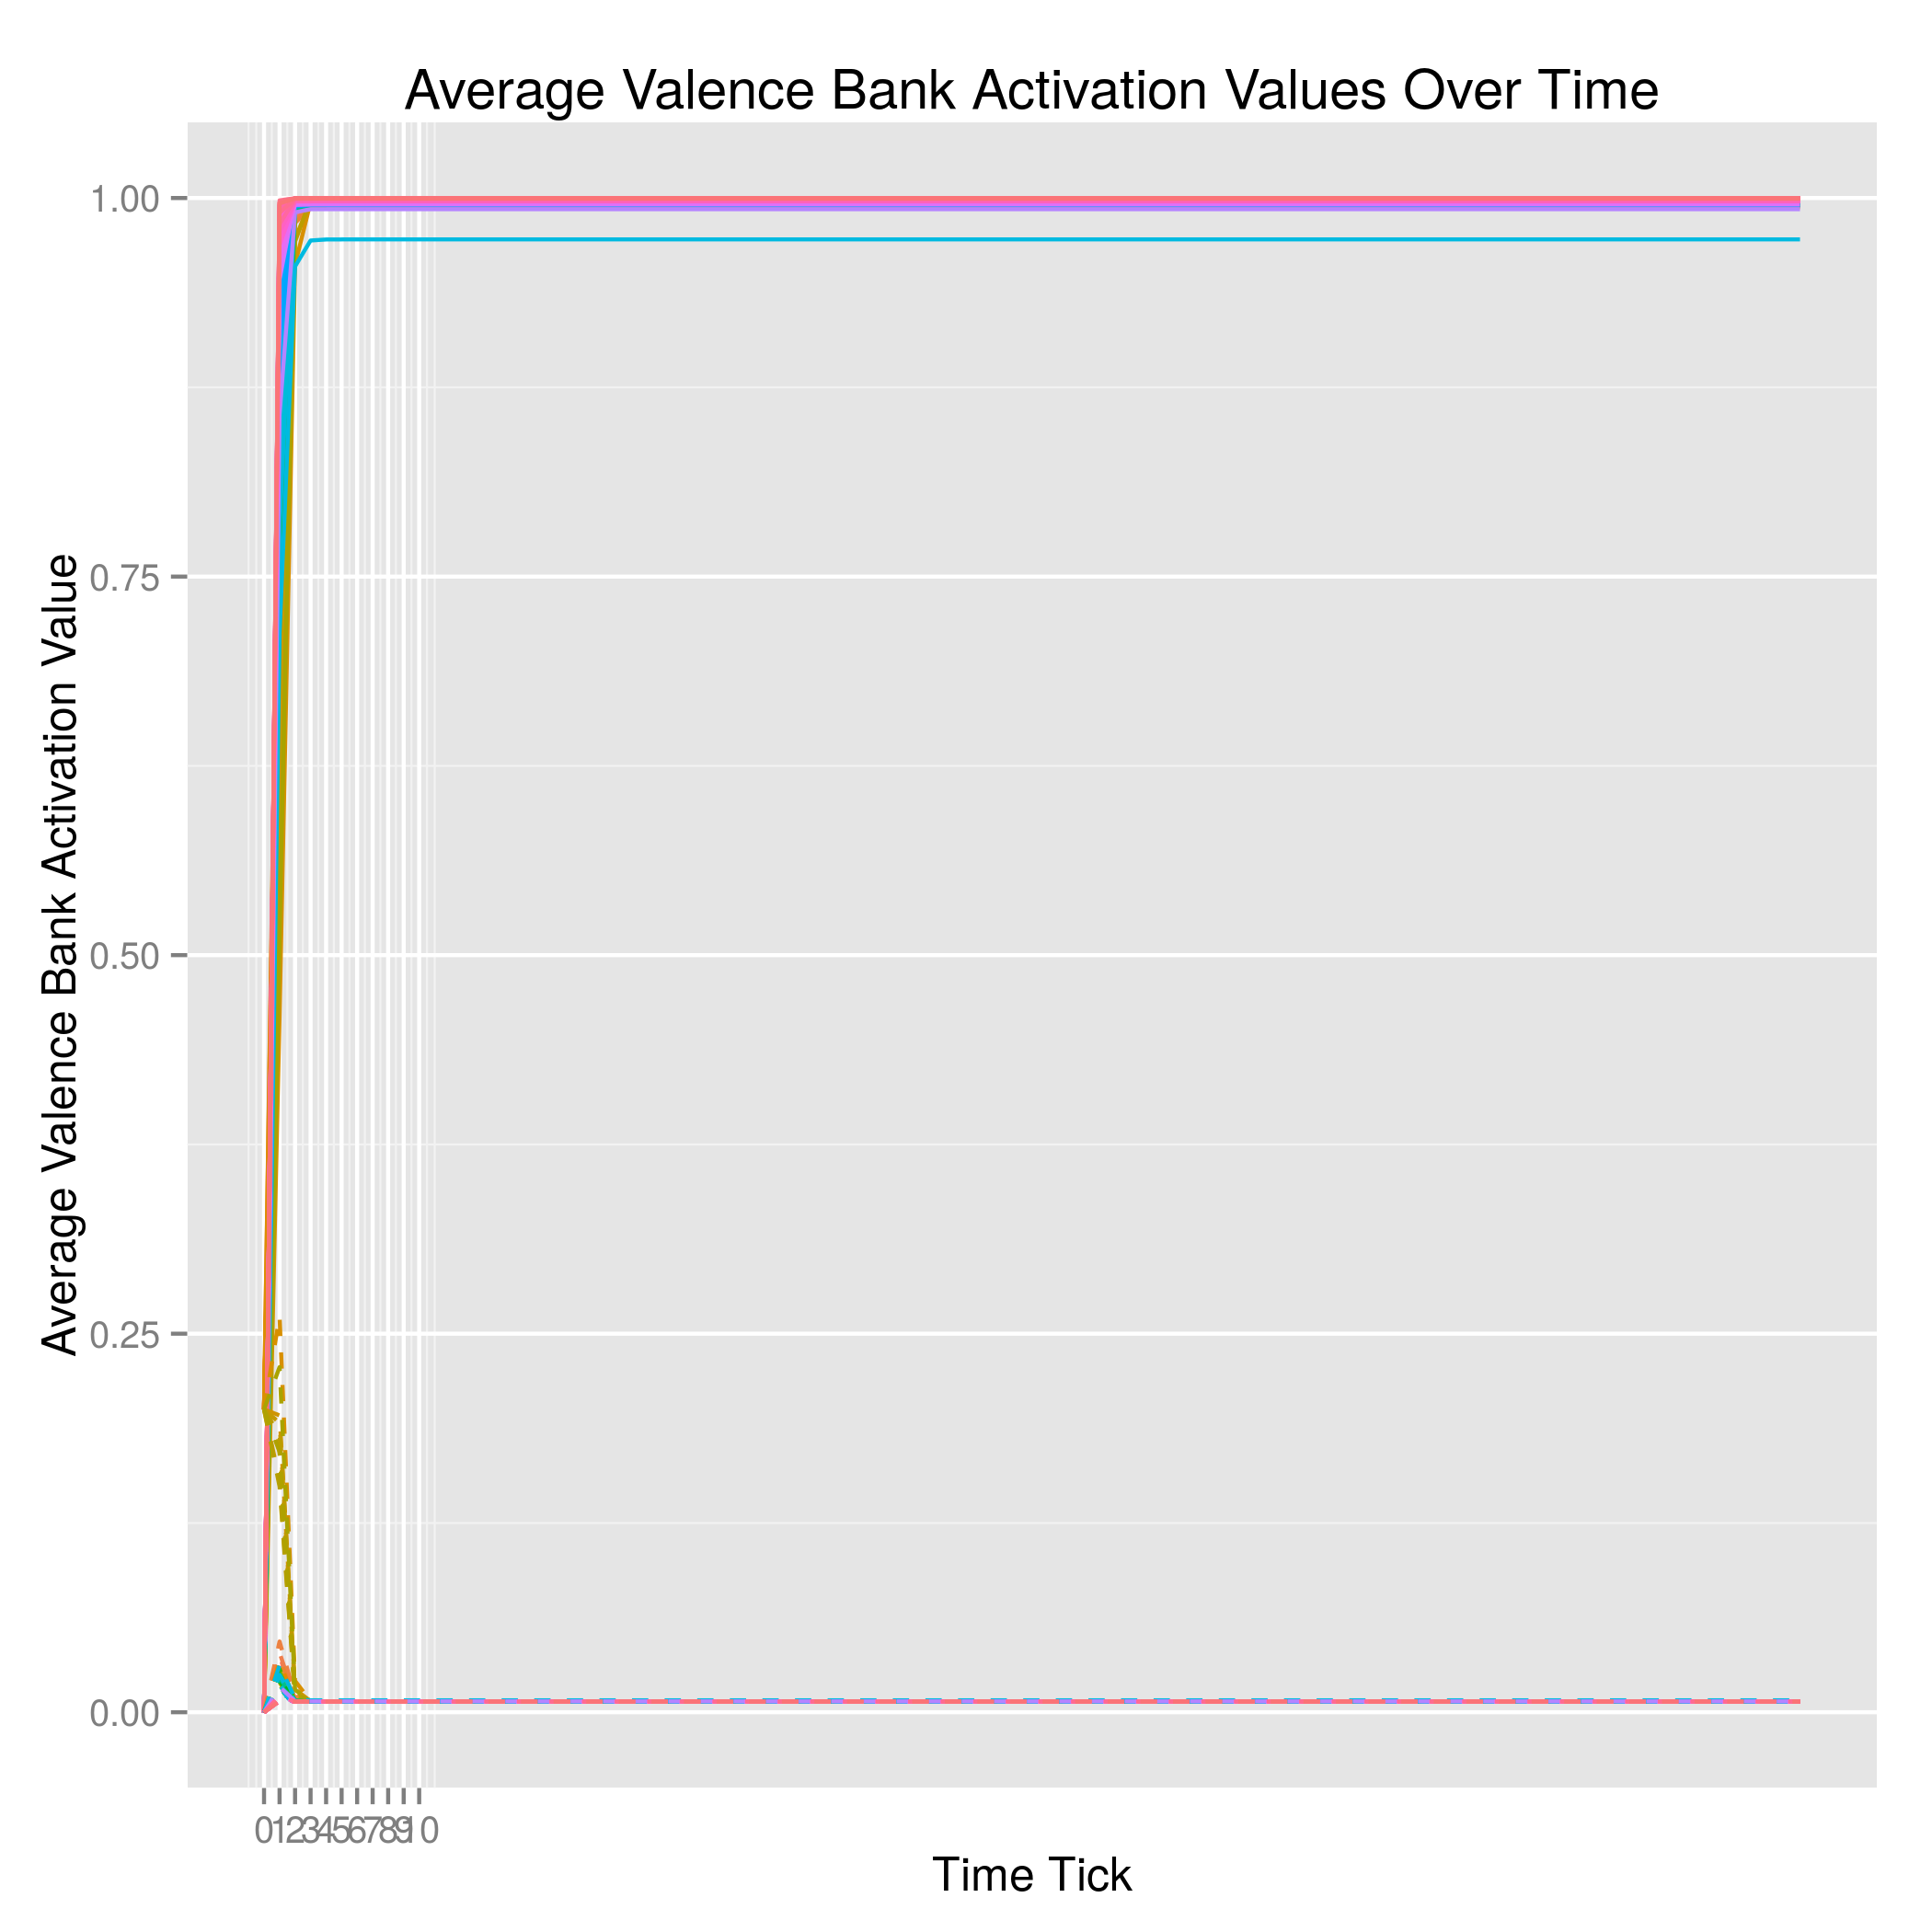
\includegraphics[width=\maxwidth]{figure/unnamed-chunk-23} 
\begin{kframe}\begin{verbatim}
## [1] 4
## [1] 30001
\end{verbatim}
\end{kframe}
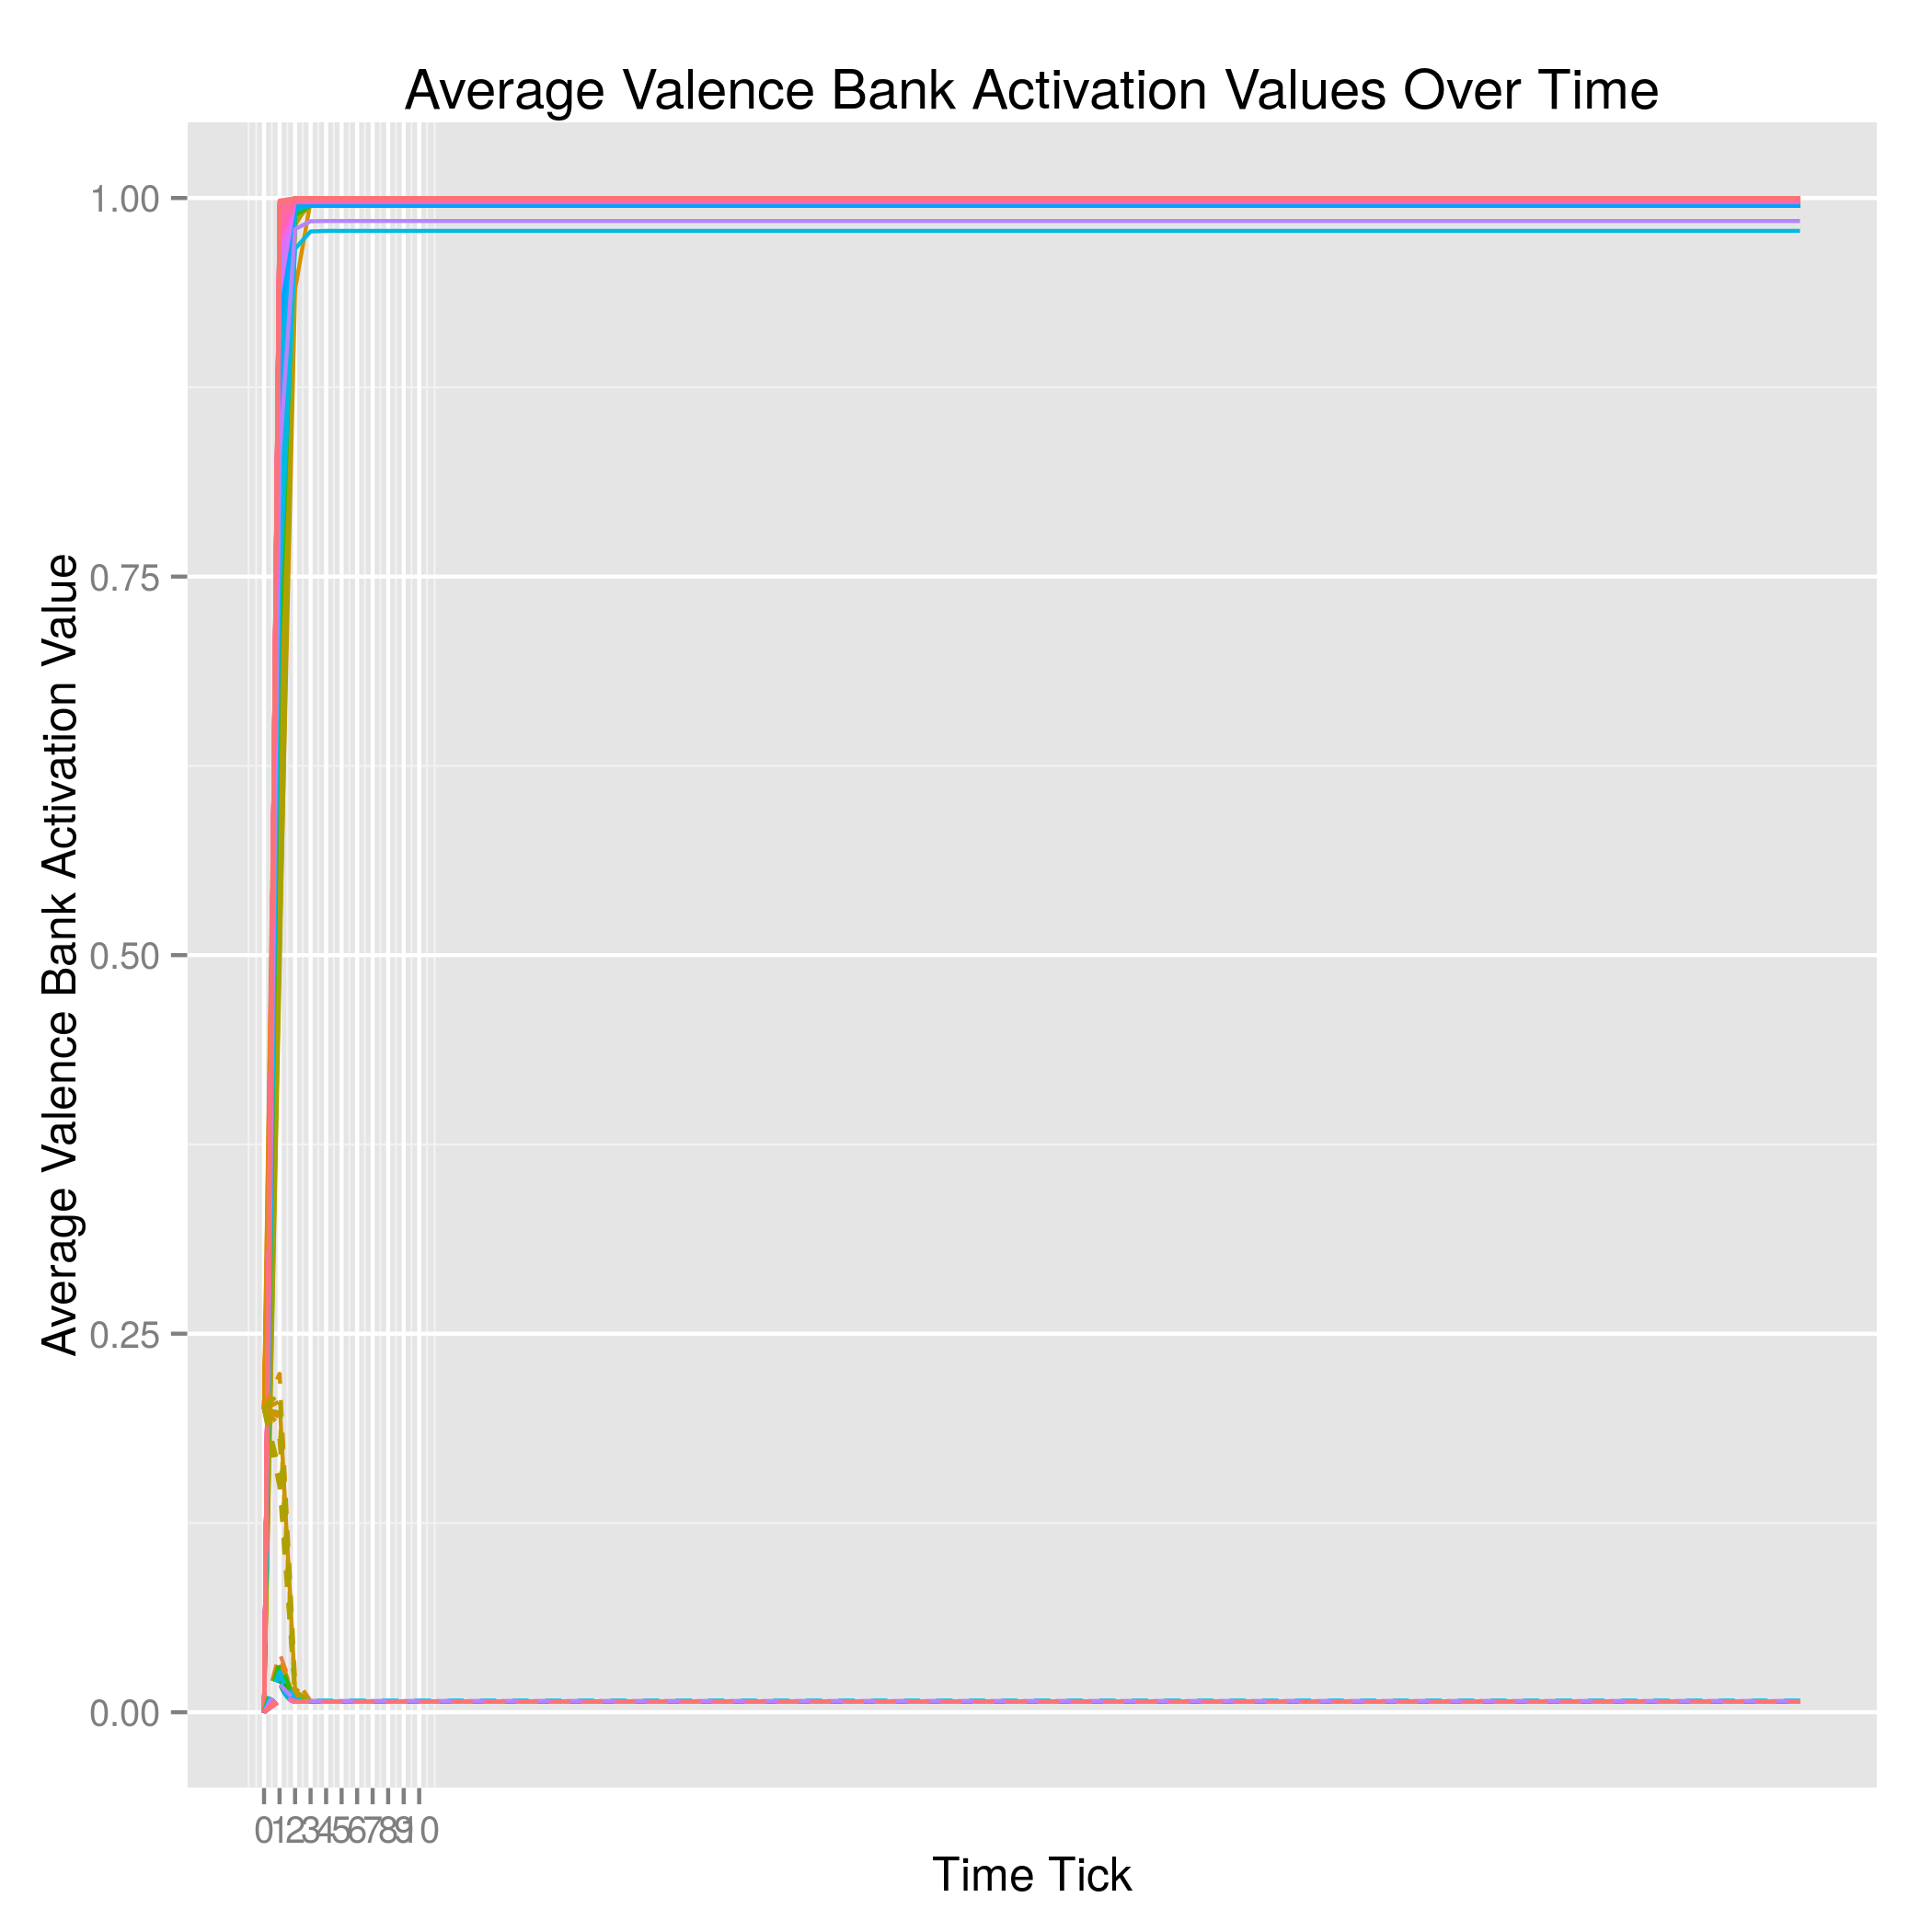
\includegraphics[width=\maxwidth]{figure/unnamed-chunk-24} 
\begin{kframe}\begin{verbatim}
## [1] 5
## [1] 40001
\end{verbatim}
\end{kframe}
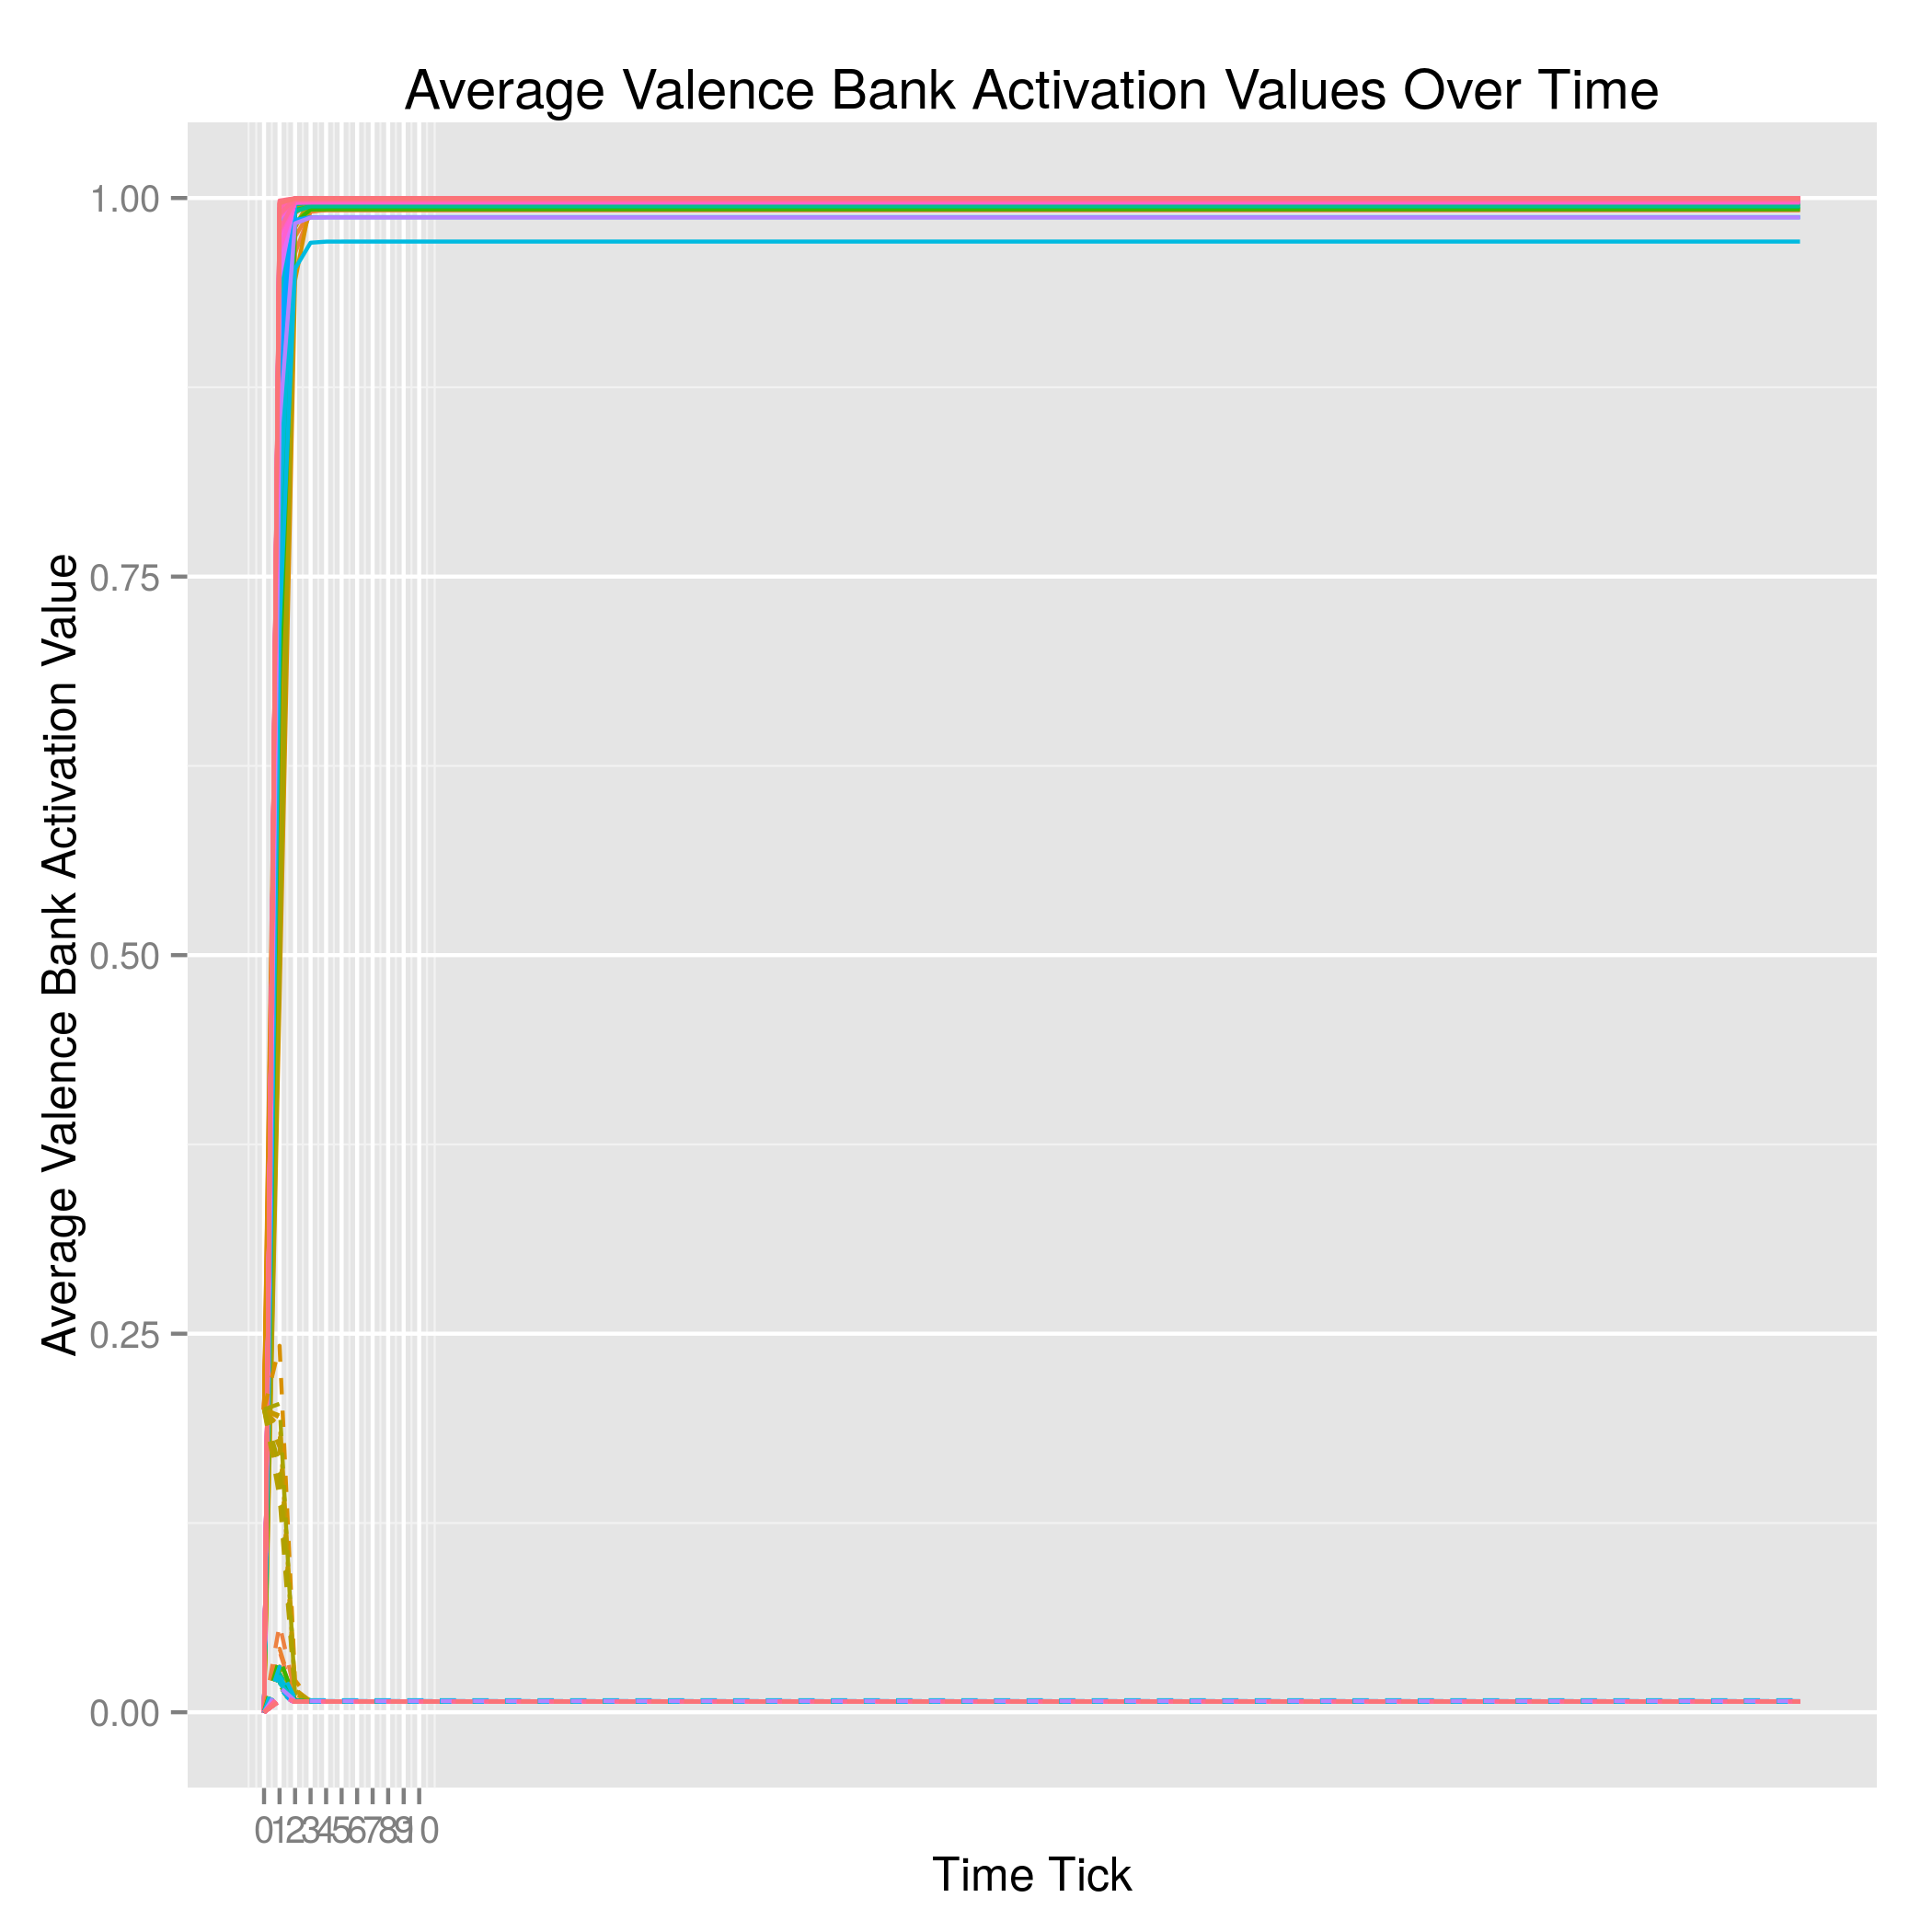
\includegraphics[width=\maxwidth]{figure/unnamed-chunk-25} 
\begin{kframe}\begin{verbatim}
## [1] 6
## [1] 50001
\end{verbatim}
\end{kframe}
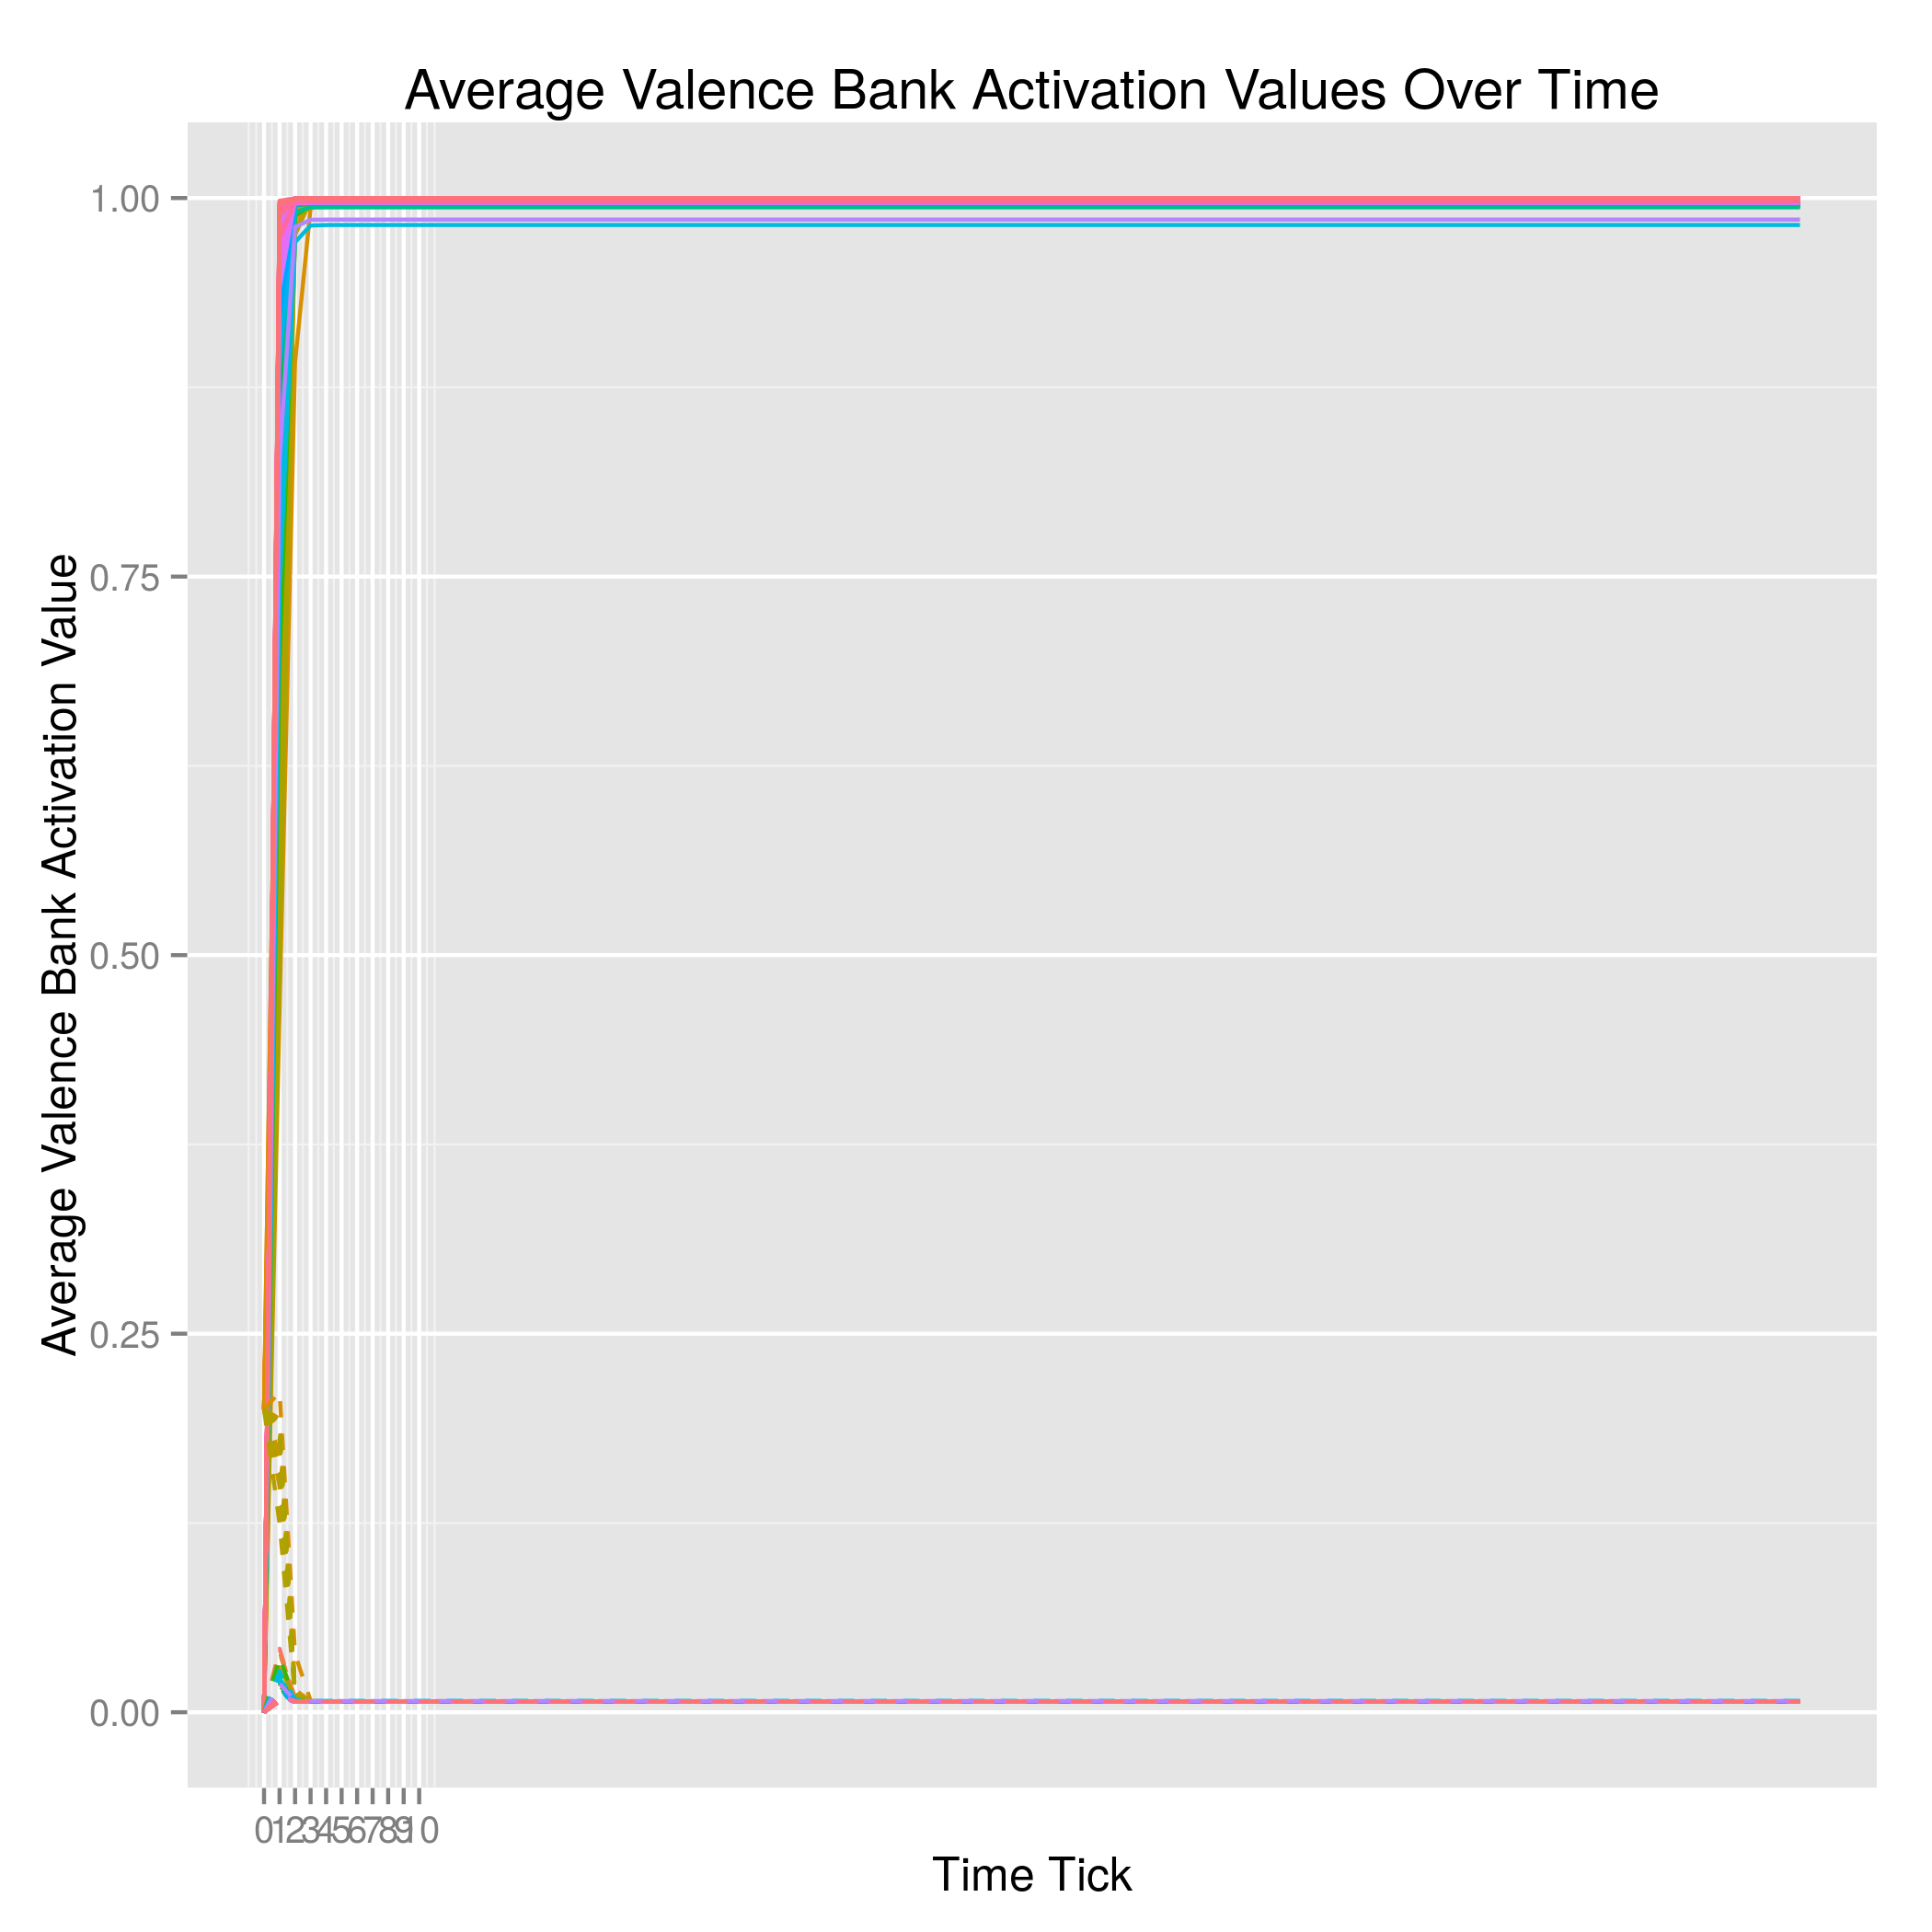
\includegraphics[width=\maxwidth]{figure/unnamed-chunk-26} 
\begin{kframe}\begin{verbatim}
## [1] 7
## [1] 60001
\end{verbatim}
\end{kframe}
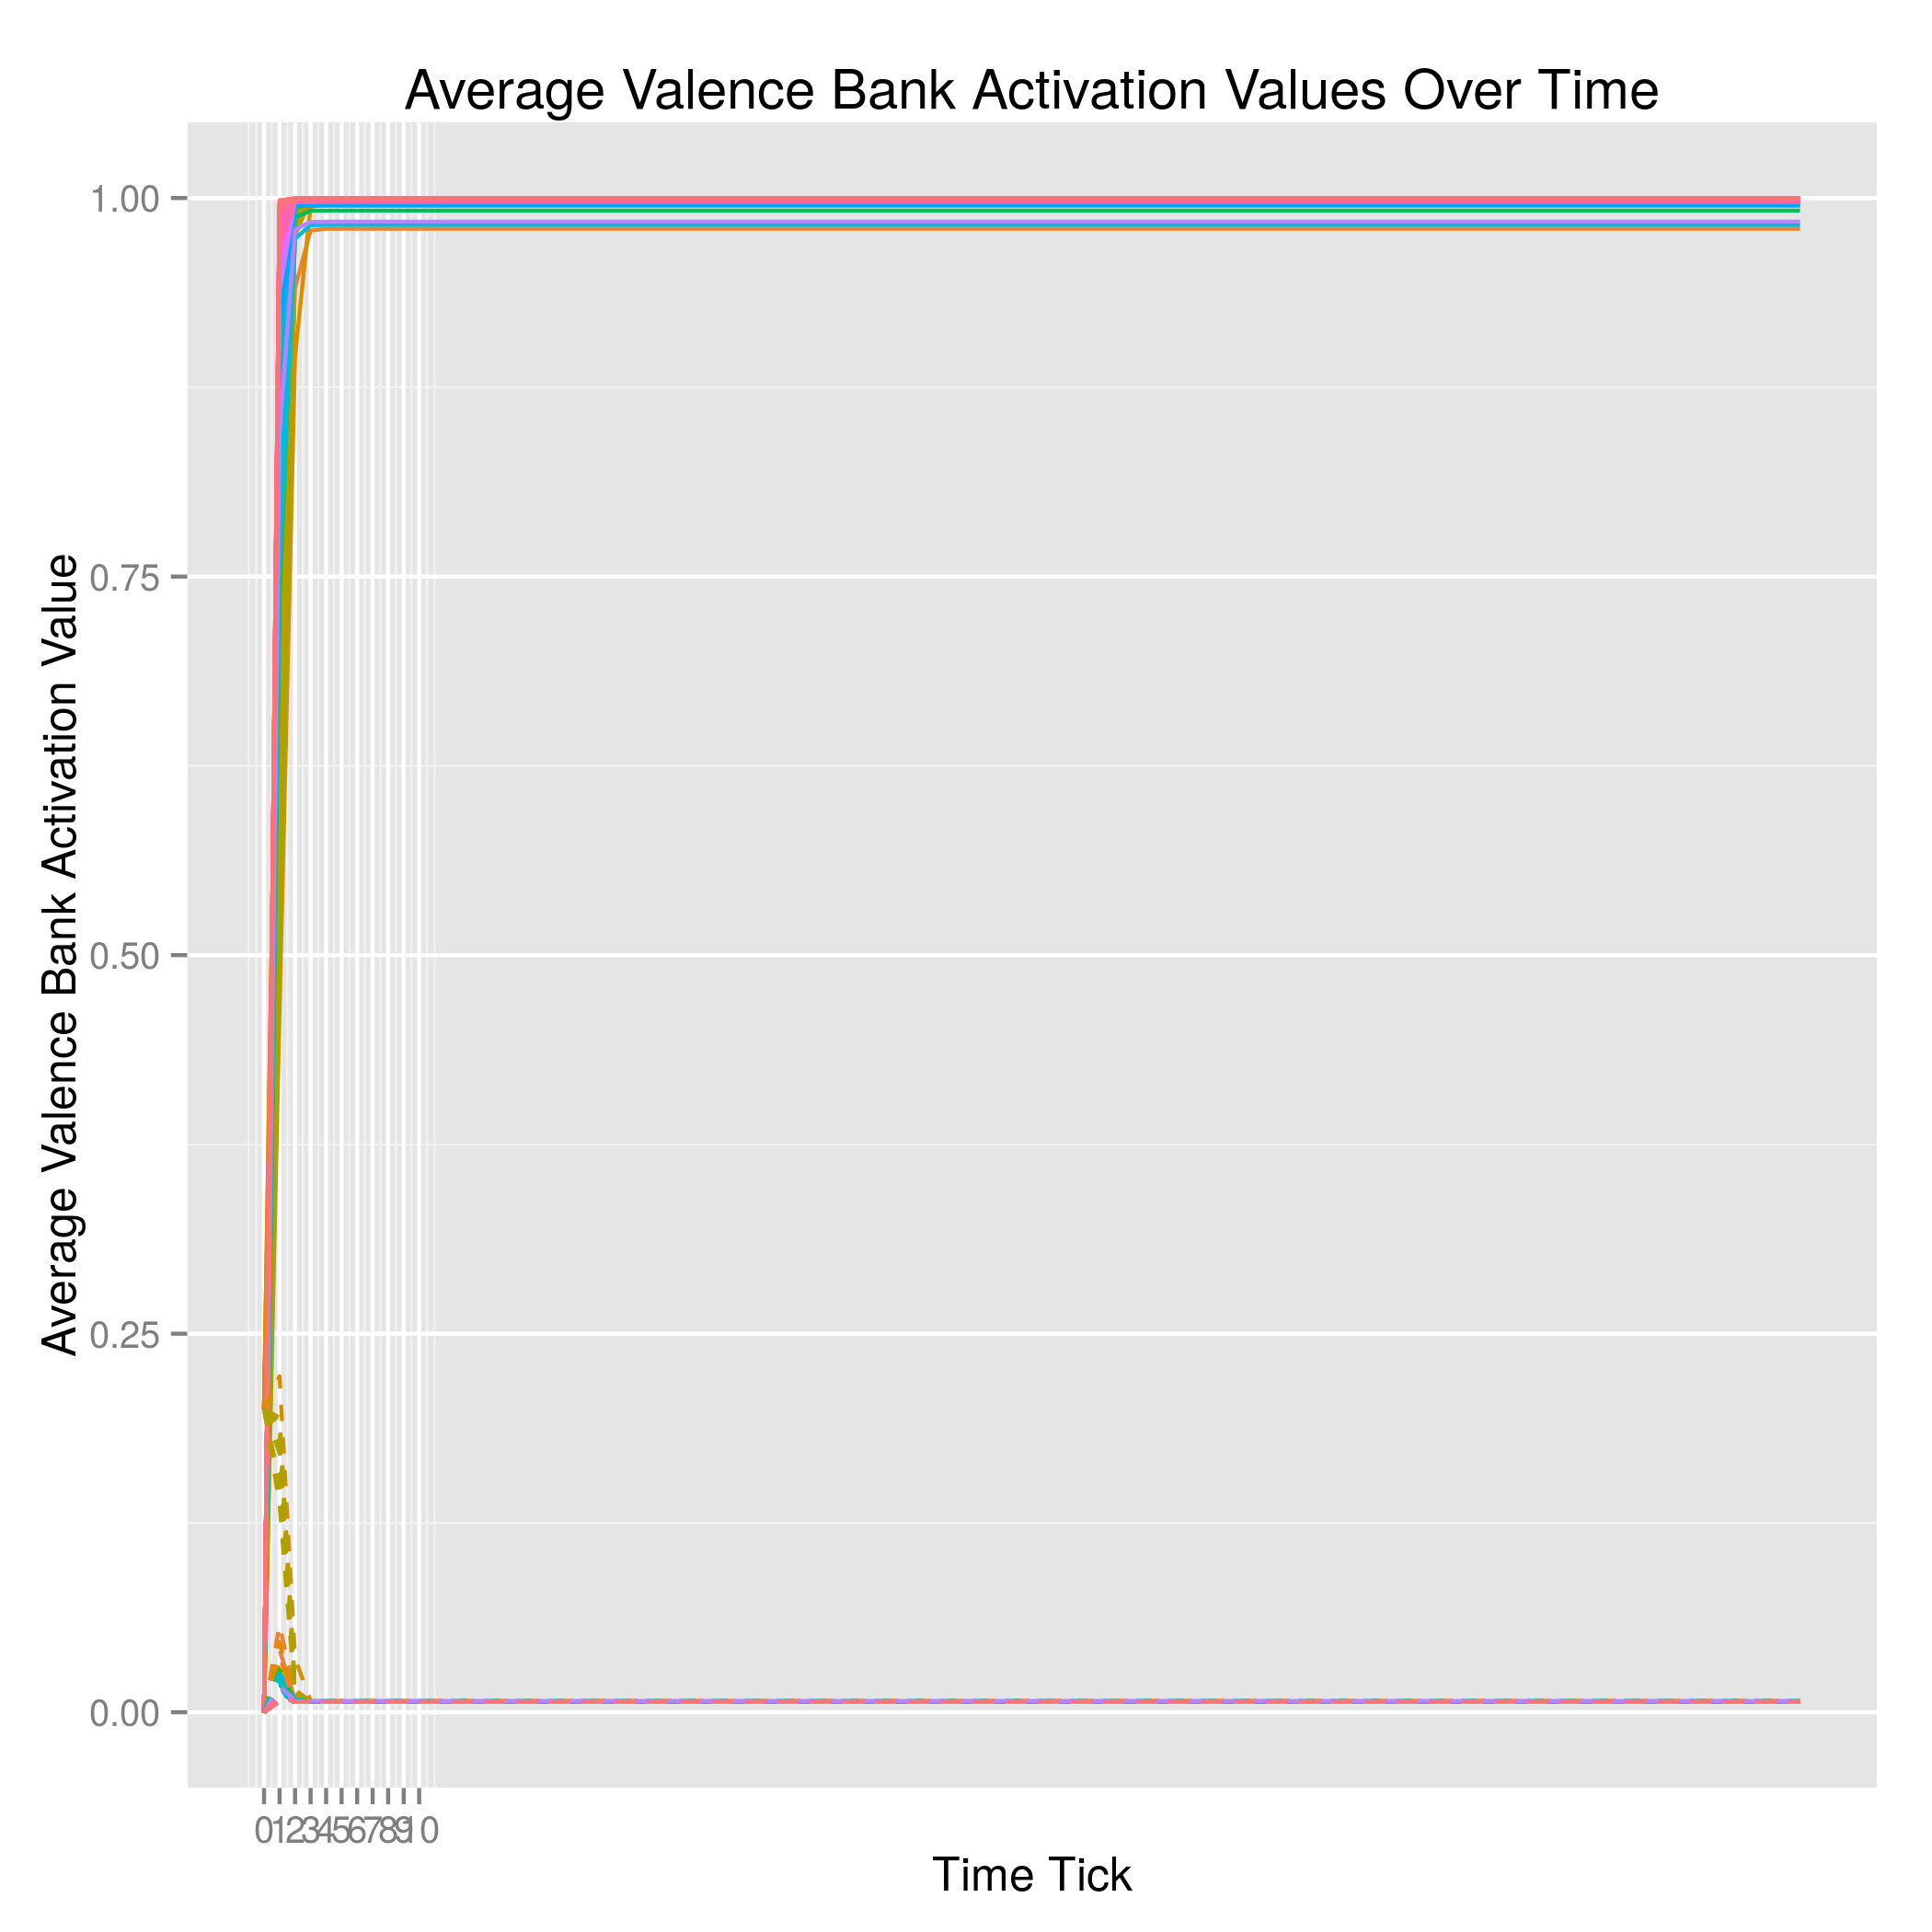
\includegraphics[width=\maxwidth]{figure/unnamed-chunk-27} 
\begin{kframe}\begin{verbatim}
## [1] 8
## [1] 70001
\end{verbatim}
\end{kframe}
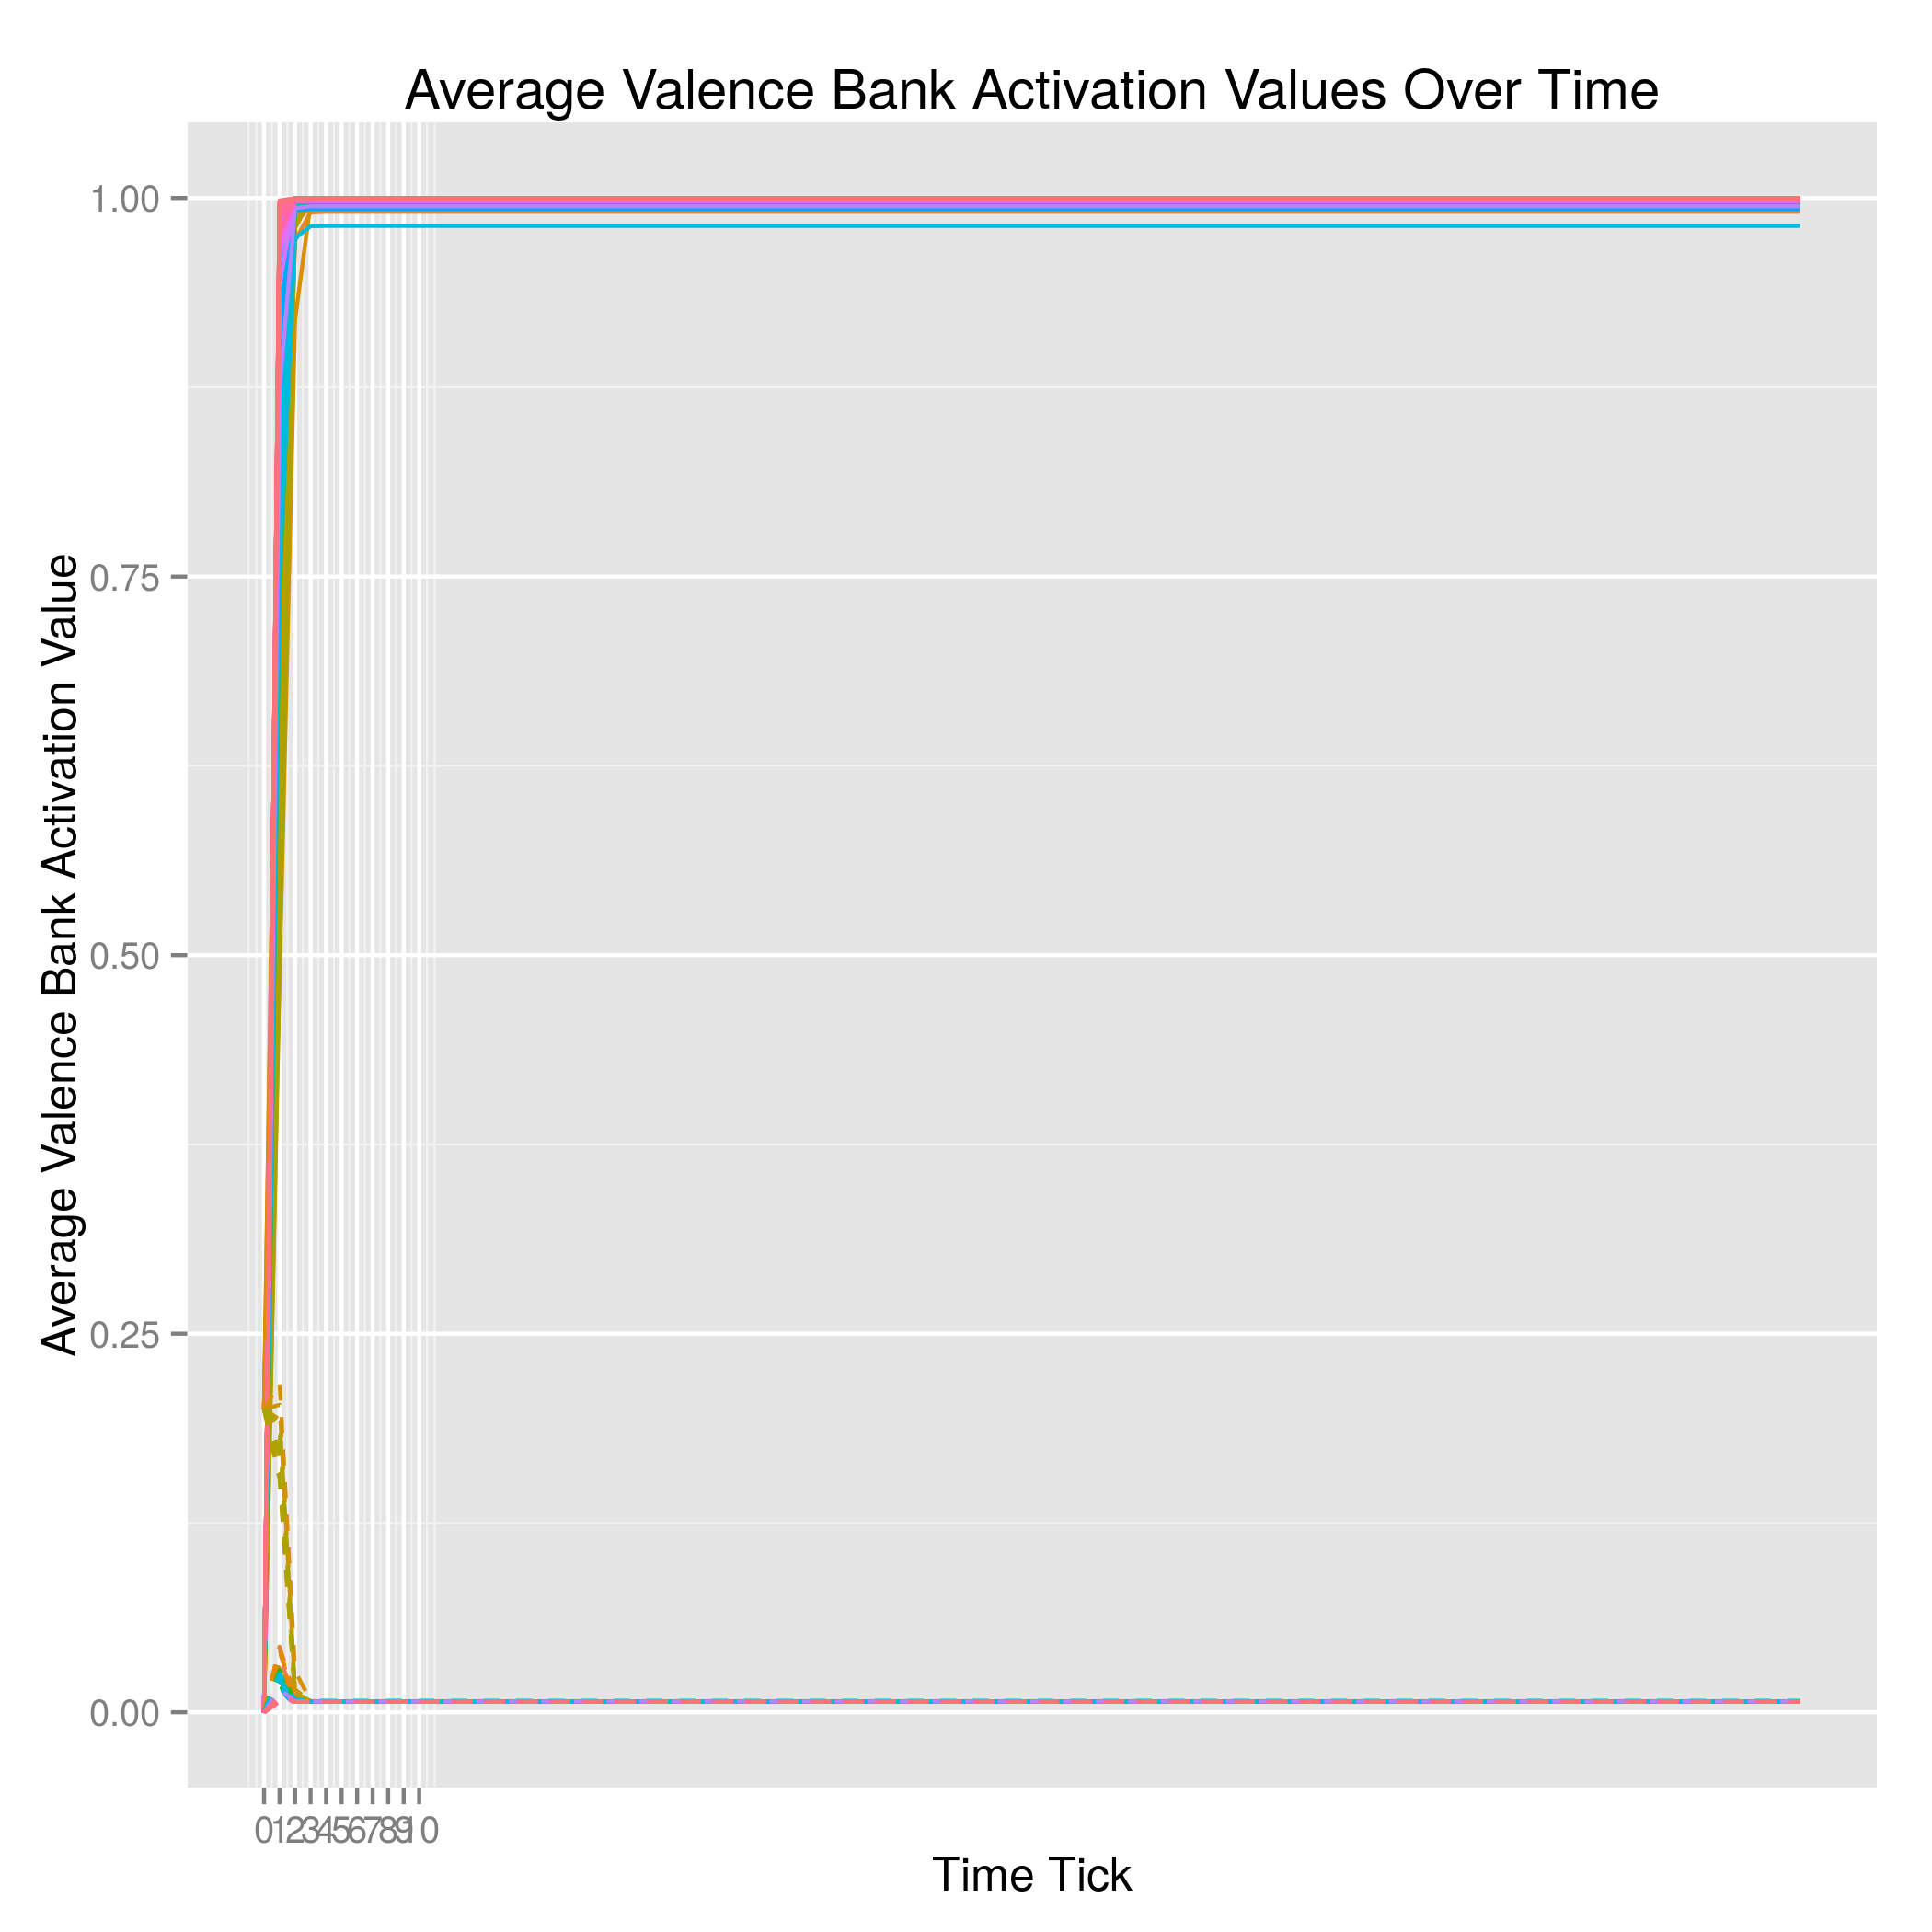
\includegraphics[width=\maxwidth]{figure/unnamed-chunk-28} 
\begin{kframe}\begin{verbatim}
## [1] 9
## [1] 80001
\end{verbatim}
\end{kframe}
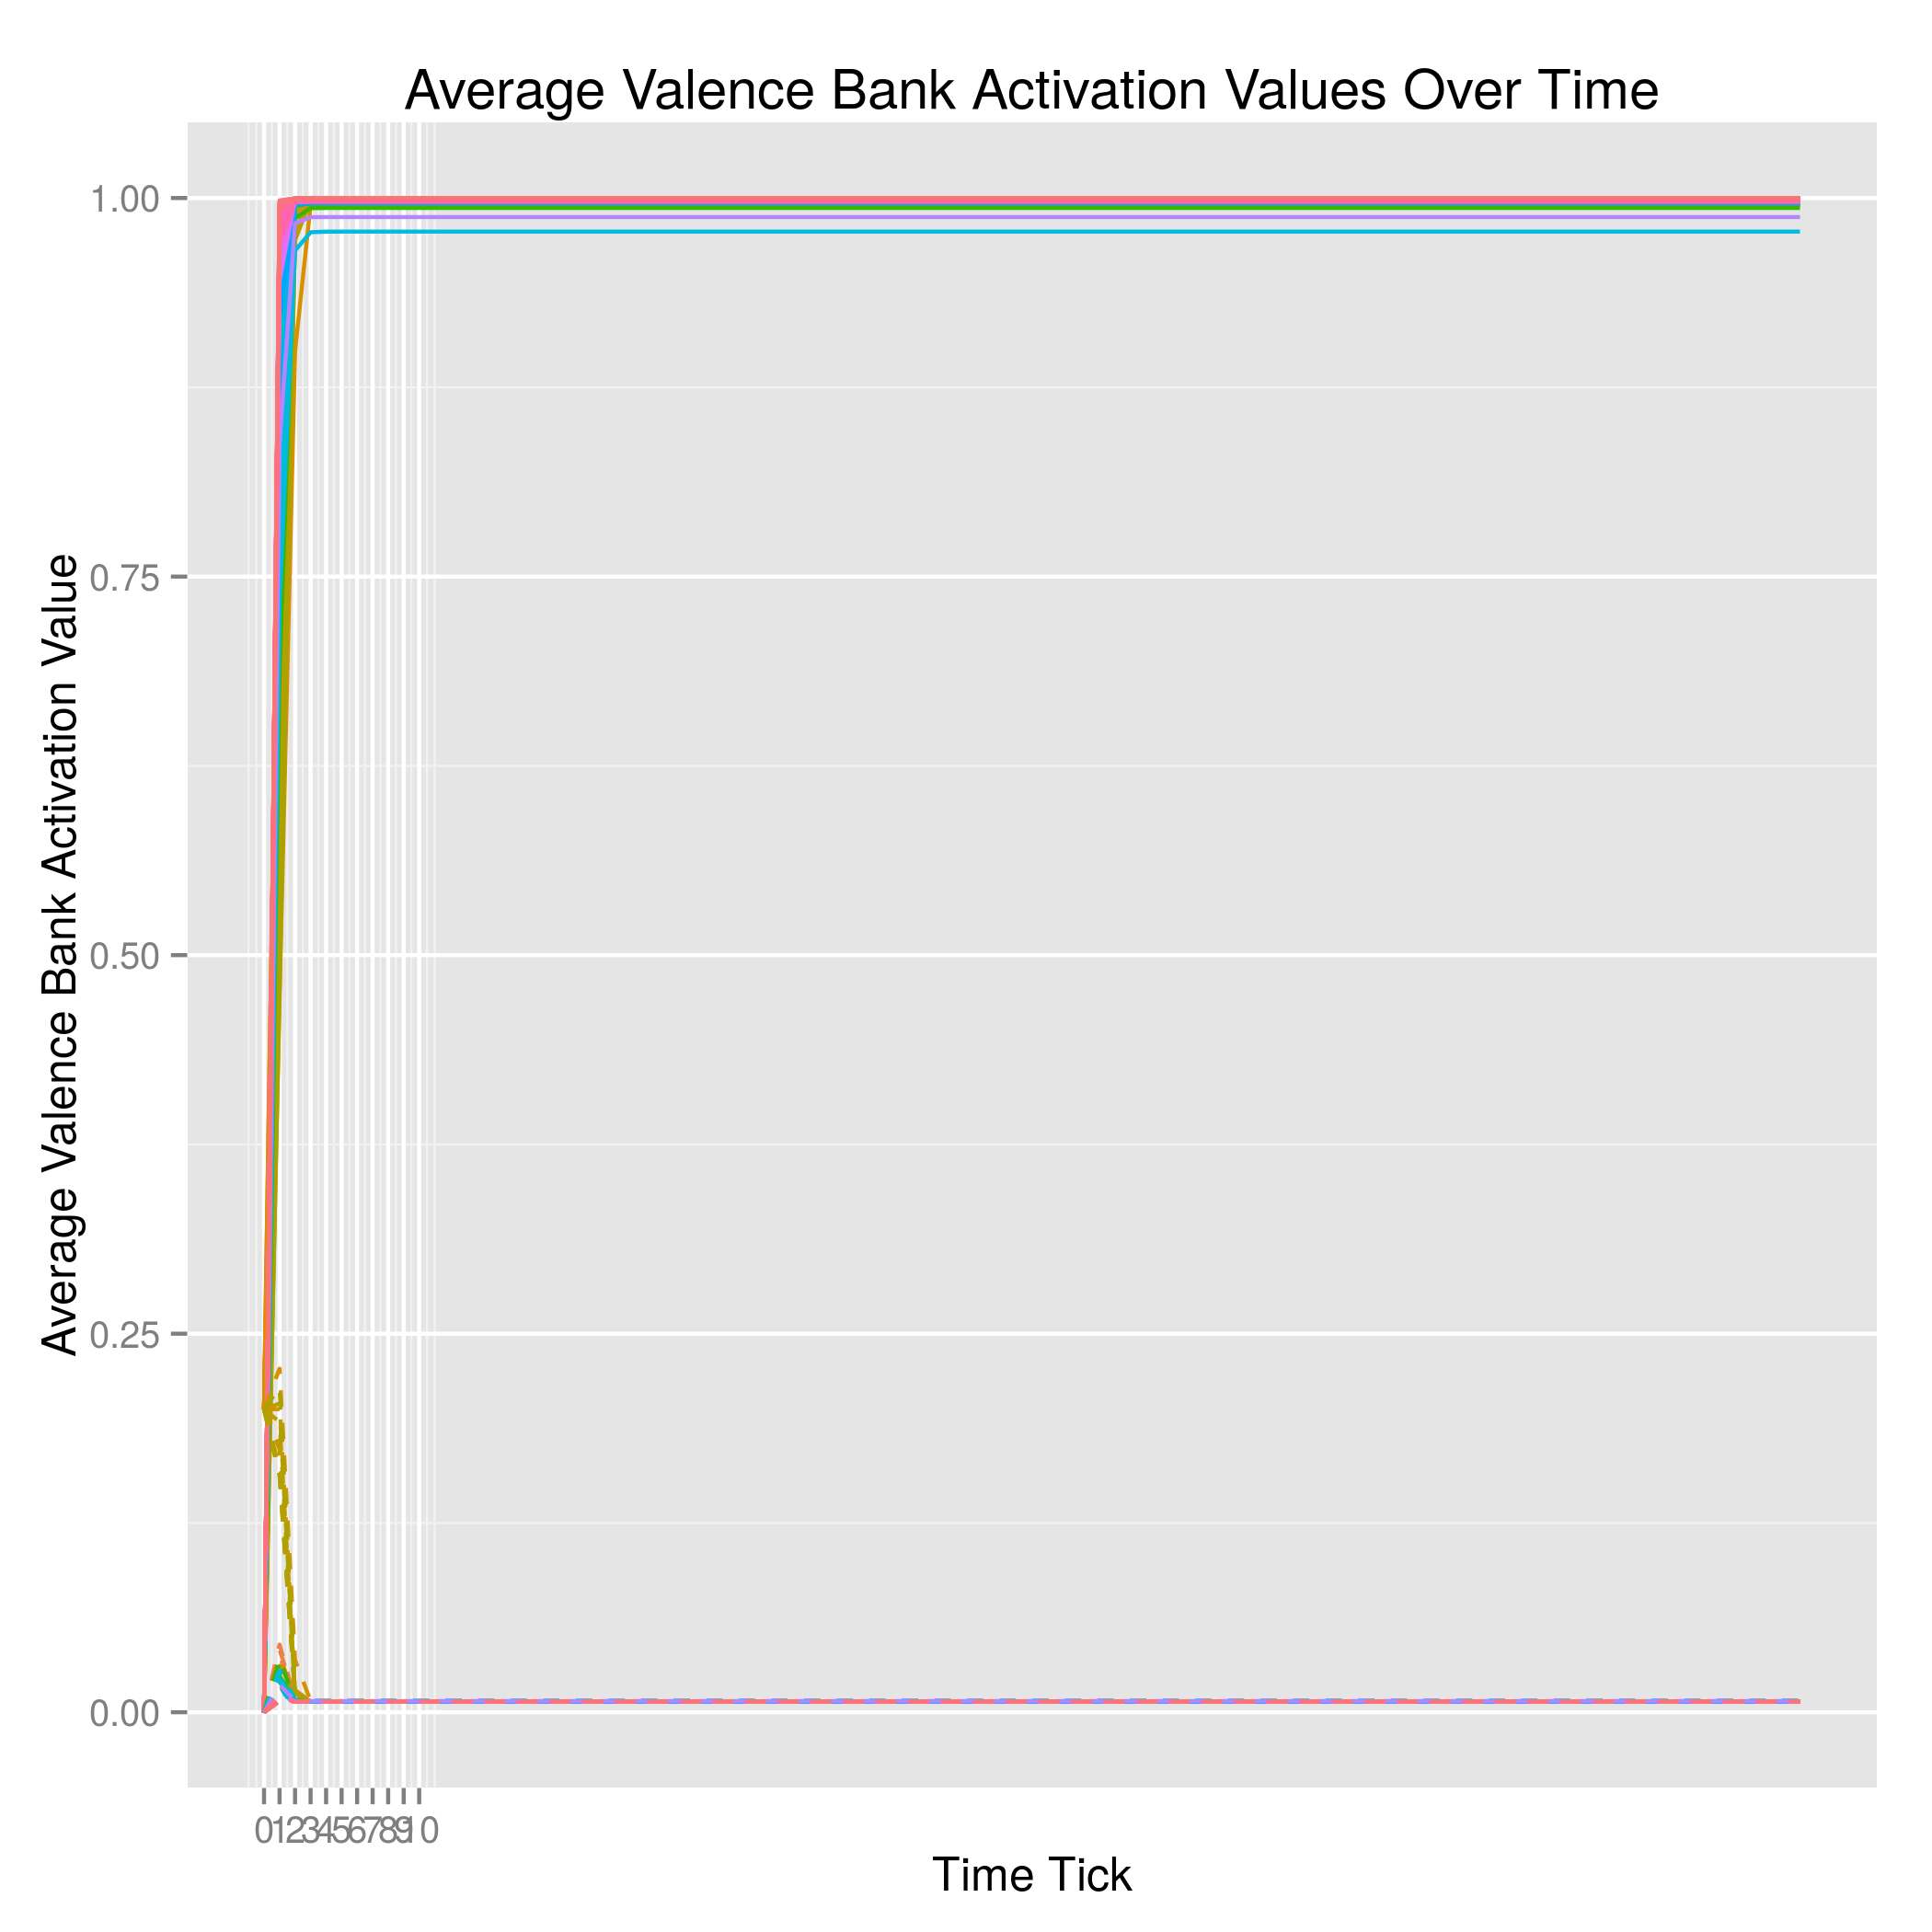
\includegraphics[width=\maxwidth]{figure/unnamed-chunk-29} 
\begin{kframe}\begin{verbatim}
## [1] 10
## [1] 90001
\end{verbatim}
\end{kframe}
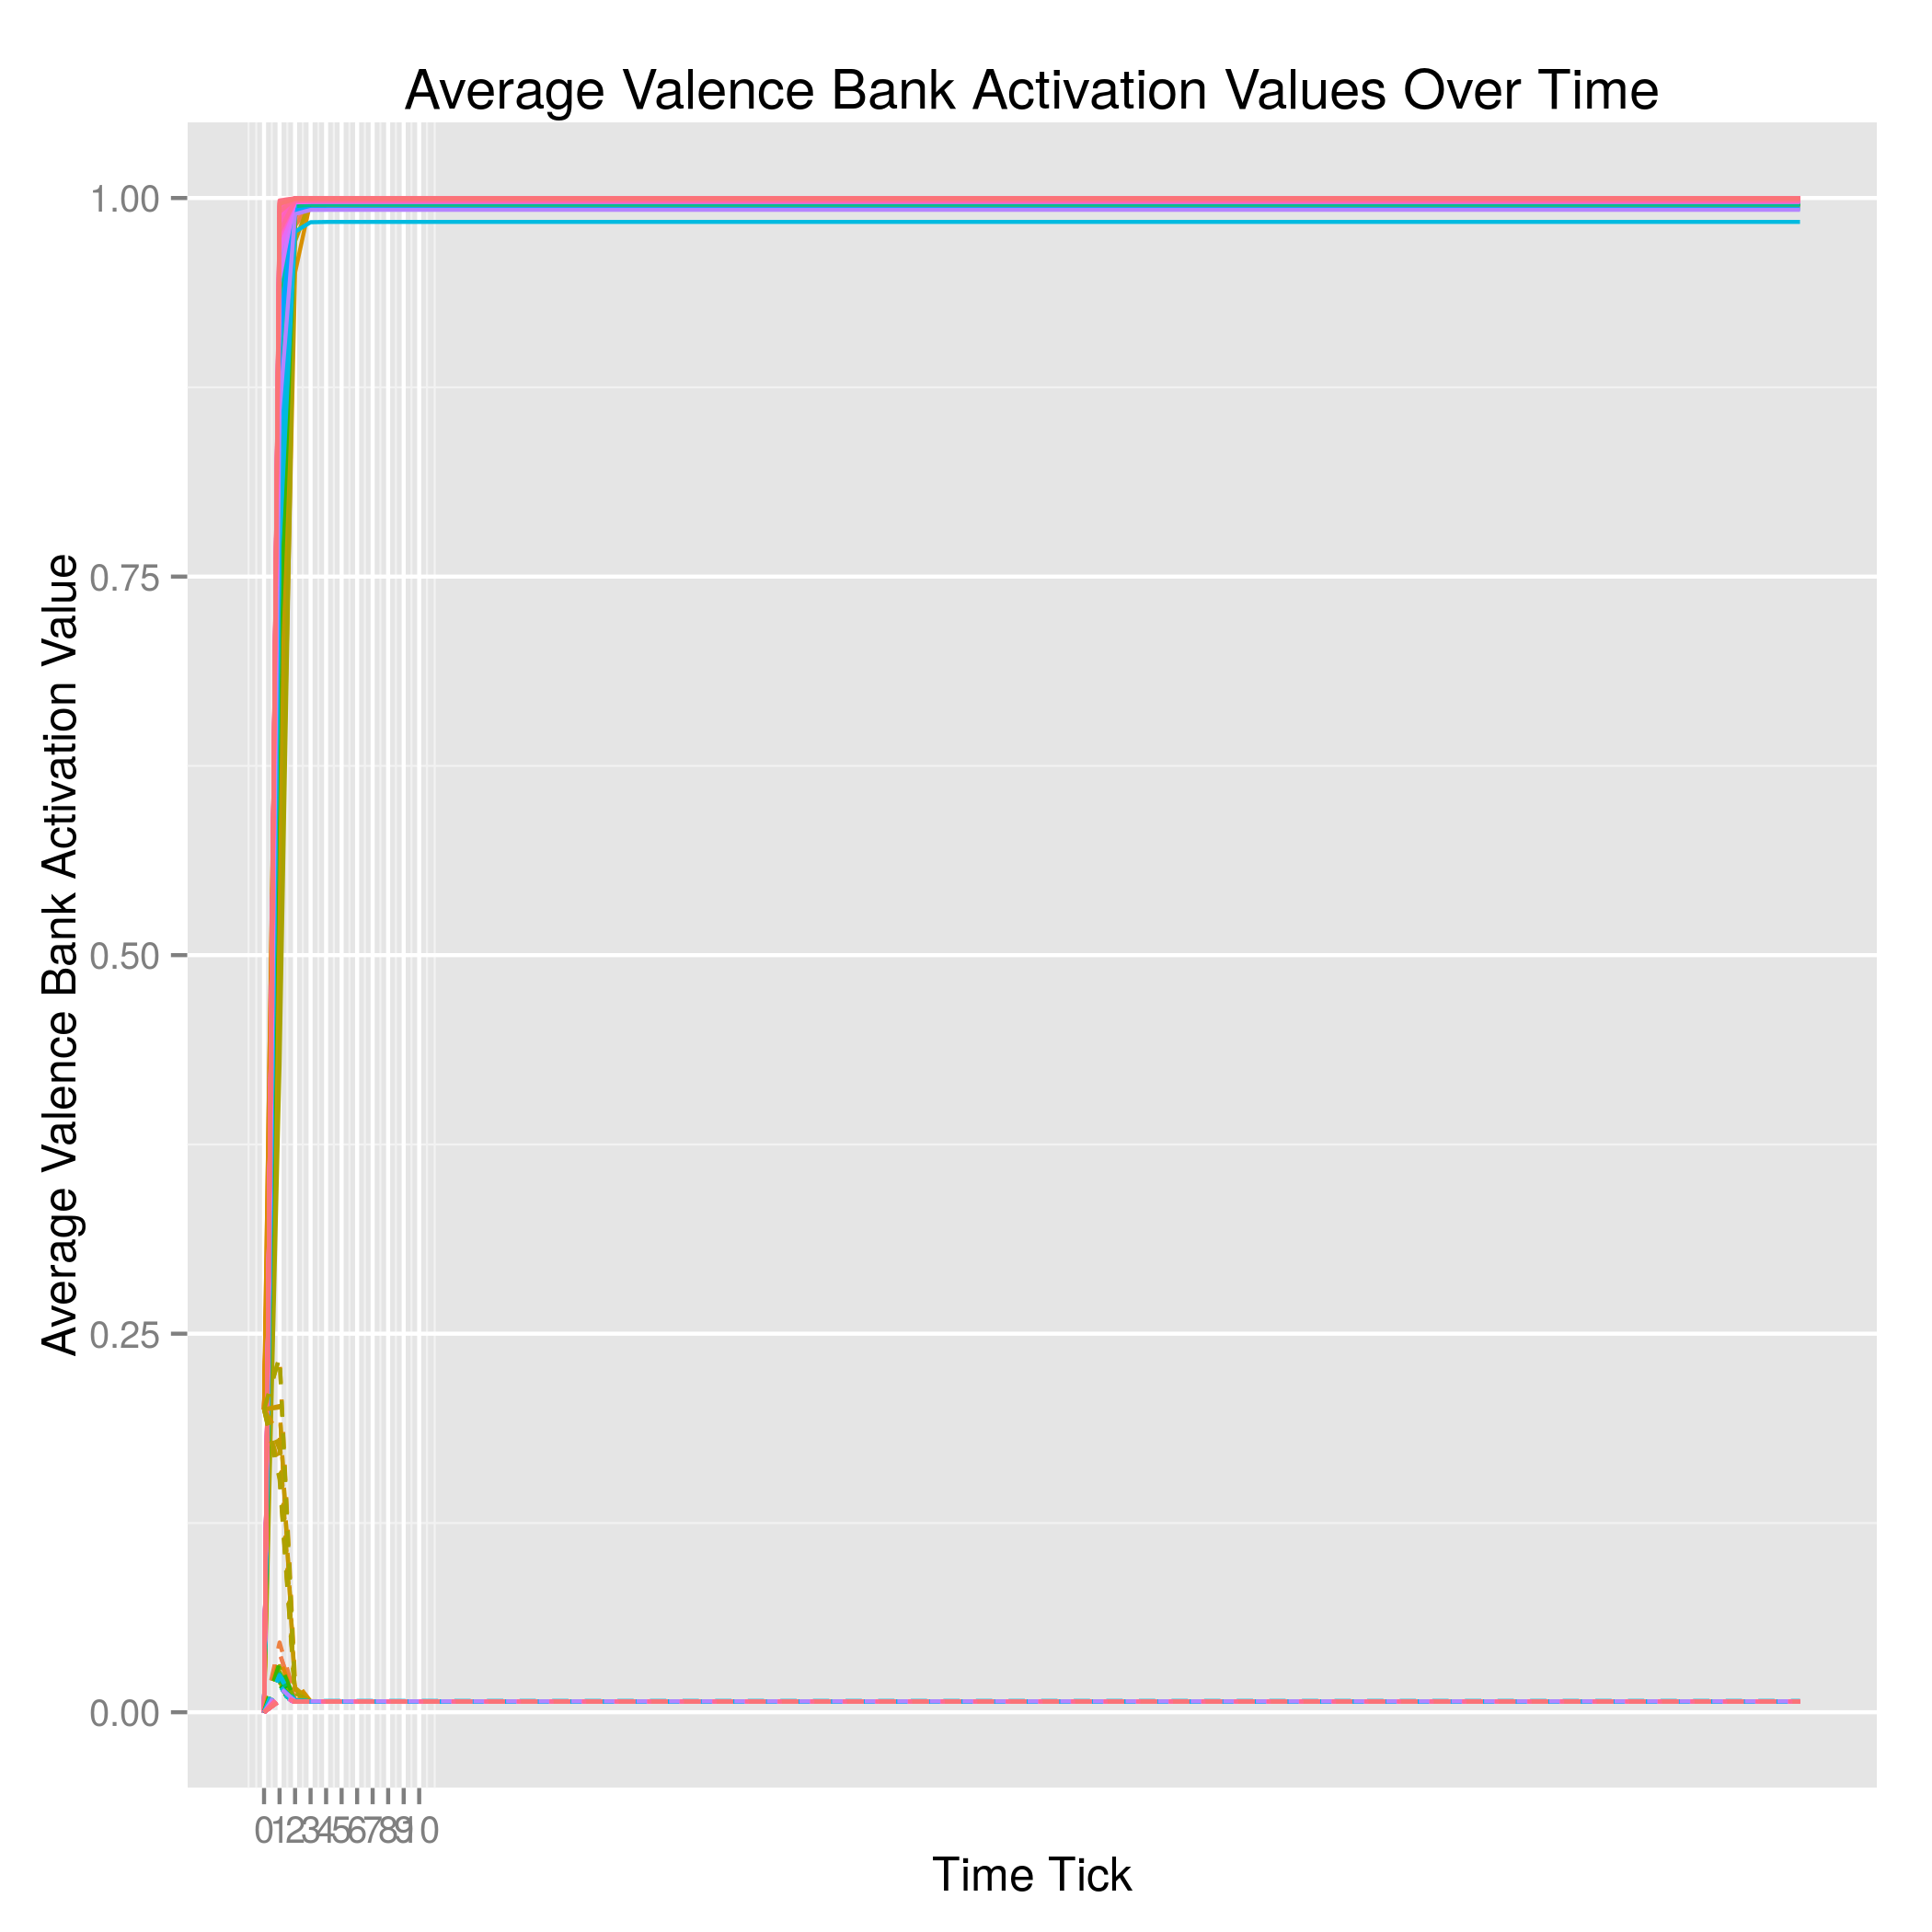
\includegraphics[width=\maxwidth]{figure/unnamed-chunk-210} 

\end{knitrout}


\end{document}
